\part{\EN{Slightly more advanced examples}\RU{Более сложные примеры}}

\newcommand{\CURPATH}{advanced/100_fahrenheit}
\EN{\section{Text strings}

\subsection{\CCpp}

\label{C_strings}
The normal C strings are zero-terminated (\ac{ASCIIZ}-strings).

The reason why the C string format is as it is (zero-terminated) is apparently historical.
In [Dennis M. Ritchie, \IT{The Evolution of the Unix Time-sharing System}, (1979)]
we read:

\begin{framed}
\begin{quotation}
A minor difference was that the unit of I/O was the word, not the byte, because the PDP-7 was a word-addressed
machine. In practice this meant merely that all programs dealing with character streams ignored null
characters, because null was used to pad a file to an even number of characters.
\end{quotation}
\end{framed}

\myindex{Hiew}

In Hiew or FAR Manager these strings looks like this:

\begin{lstlisting}
int main()
{
	printf ("Hello, world!\n");
};
\end{lstlisting}

\begin{figure}[H]
\centering
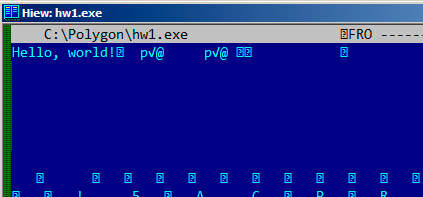
\includegraphics[scale=\NormalScale]{digging_into_code/strings/C-string.png}
\caption{Hiew}
\end{figure}

% FIXME видно \n в конце, потом пробел

\subsection{Borland Delphi}
\myindex{Pascal}
\myindex{Borland Delphi}

The string in Pascal and Borland Delphi is preceded by an 8-bit or 32-bit string length.

For example:

\begin{lstlisting}[caption=Delphi]
CODE:00518AC8                 dd 19h
CODE:00518ACC aLoading___Plea db 'Loading... , please wait.',0

...

CODE:00518AFC                 dd 10h
CODE:00518B00 aPreparingRun__ db 'Preparing run...',0
\end{lstlisting}

\subsection{Unicode}

\myindex{Unicode}

Often, what is called Unicode is a methods for encoding strings where each character occupies 2 bytes or 16 bits.
This is a common terminological mistake.
Unicode is a standard for assigning a number to each character in the many writing systems of the 
world, but does not describe the encoding method.

\myindex{UTF-8}
\myindex{UTF-16LE}
The most popular encoding methods are: UTF-8 (is widespread in Internet and *NIX systems) and UTF-16LE (is used in Windows).

\subsubsection{UTF-8}

\myindex{UTF-8}
UTF-8 is one of the most successful methods for
encoding characters.
All Latin symbols are encoded just like in ASCII,
and the symbols beyond the ASCII table are encoded using several bytes.
0 is encoded as
before, so all standard C string functions work with UTF-8 strings just like any other string.

Let's see how the symbols in various languages are encoded in UTF-8 and how it looks like in FAR, using the 437 codepage
\footnote{The example and translations was taken from here: 
\url{http://go.yurichev.com/17304}}:

\begin{figure}[H]
\centering

\includegraphics[scale=\NormalScale]{digging_into_code/strings/multilang_sampler.png}
\end{figure}

% FIXME: cut it
\begin{figure}[H]
\centering
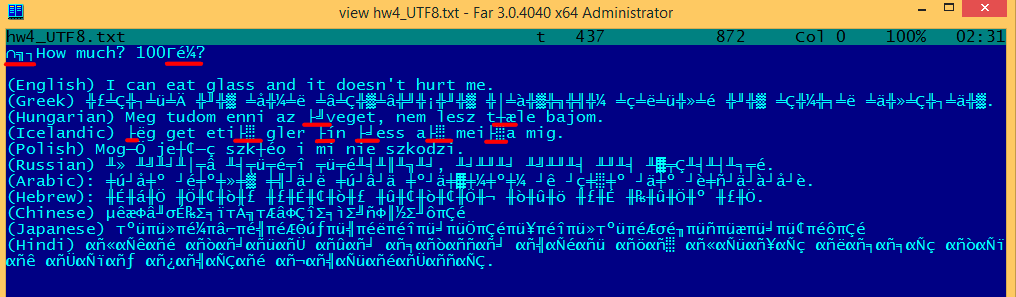
\includegraphics[scale=\FigScale]{digging_into_code/strings/multilang_sampler_UTF8.png}
\caption{FAR: UTF-8}
\end{figure}

As you can see, the English language string looks the same as it is in ASCII.

The Hungarian language uses some Latin symbols plus symbols with diacritic marks.

These symbols are encoded using several bytes, these are underscored with red.
It's the same story with the Icelandic and Polish languages.

There is also the \q{Euro} currency symbol at the start, which is encoded with 3 bytes.

The rest of the writing systems here have no connection with Latin.

At least in Russian, Arabic, Hebrew and Hindi we can see some recurring bytes, and that is not surprise:
all symbols from a writing system are usually located in the same Unicode table, so their code begins with
the same numbers.

At the beginning, before the \q{How much?} string we see 3 bytes, which are in fact the \ac{BOM}.
The \ac{BOM} defines the encoding system to be
used.

\subsubsection{UTF-16LE}

\myindex{UTF-16LE}
\myindex{Windows!Win32}
Many win32 functions in Windows have the suffixes \TT{-A} and \TT{-W}.
The first type of functions works
with normal strings, the other with UTF-16LE strings (\IT{wide}).

In the second case, each symbol is usually stored in a 16-bit value of type \IT{short}.

The Latin symbols in UTF-16 strings look in Hiew or FAR like they are interleaved with zero byte:

\begin{lstlisting}
int wmain()
{
	wprintf (L"Hello, world!\n");
};
\end{lstlisting}

\begin{figure}[H]
\centering
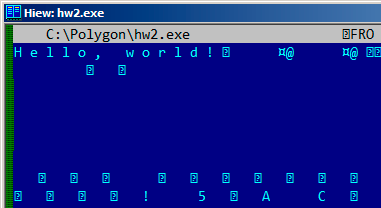
\includegraphics[scale=\NormalScale]{digging_into_code/strings/UTF16-string.png}
\caption{Hiew}
\end{figure}

We can see this often in \gls{Windows NT} system files:

\begin{figure}[H]
\centering
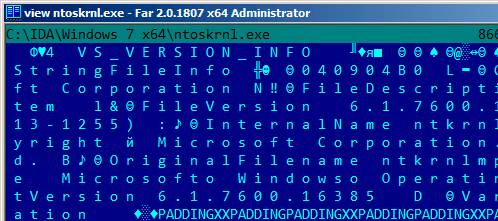
\includegraphics[scale=\NormalScale]{digging_into_code/strings/ntoskrnl_UTF16.png}
\caption{Hiew}
\end{figure}

\myindex{IDA}
Strings with characters that occupy exactly 2 bytes are called \q{Unicode} in \IDA:

\begin{lstlisting}
.data:0040E000 aHelloWorld:
.data:0040E000                 unicode 0, <Hello, world!>
.data:0040E000                 dw 0Ah, 0
\end{lstlisting}

Here is how the Russian language string is encoded in UTF-16LE:

\begin{figure}[H]
\centering
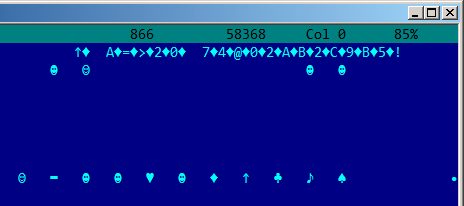
\includegraphics[scale=\NormalScale]{digging_into_code/strings/russian_UTF16.png}
\caption{Hiew: UTF-16LE}
\end{figure}

What we can easily spot is that the symbols are interleaved by the diamond character (which has the ASCII code of 4).
Indeed, the Cyrillic symbols are located in the fourth Unicode plane
\footnote{\href{http://go.yurichev.com/17003}{wikipedia}}.
Hence, all Cyrillic symbols in UTF-16LE are located in the \TT{0x400-0x4FF} range.

Let's go back to the example with the string written in multiple languages.
Here is how it looks like in UTF-16LE.

% FIXME: cut it
\begin{figure}[H]
\centering
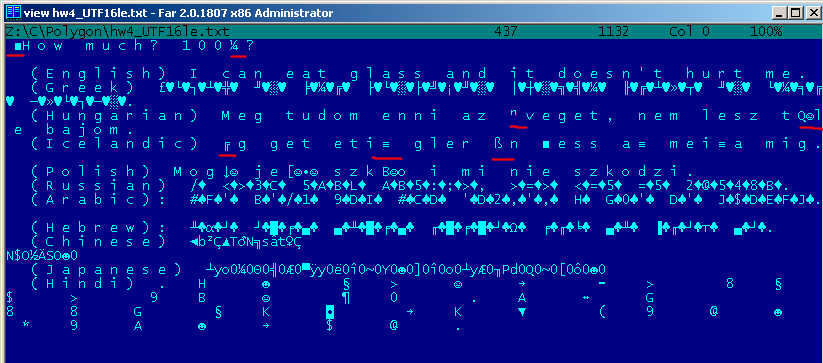
\includegraphics[scale=\FigScale]{digging_into_code/strings/multilang_sampler_UTF16.png}
\caption{FAR: UTF-16LE}
\end{figure}

Here we can also see the \ac{BOM} in the beginning.
All Latin characters are interleaved with a zero byte.

Some characters with diacritic marks (Hungarian and Icelandic languages) are also underscored in red.

% TODO: strings *NIX utility. procmonitor also shows strings...

% subsection:
\subsection{Base64}
\myindex{Base64}

The base64 encoding is highly popular for the cases when you need to transfer binary data as a text string.

In essence, this algorithm encodes 3 binary bytes into 4 printable characters:
all 26 Latin letters (both lower and upper case), digits, plus sign (\q{+}) and slash sign (\q{/}),
64 characters in total.

One distinctive feature of base64 strings is that they often (but not always) ends with 1 or 2 \gls{padding}
equality symbol(s) (\q{=}), for example:

\begin{lstlisting}
AVjbbVSVfcUMu1xvjaMgjNtueRwBbxnyJw8dpGnLW8ZW8aKG3v4Y0icuQT+qEJAp9lAOuWs=
\end{lstlisting}

\begin{lstlisting}
WVjbbVSVfcUMu1xvjaMgjNtueRwBbxnyJw8dpGnLW8ZW8aKG3v4Y0icuQT+qEJAp9lAOuQ==
\end{lstlisting}

The equality sign (\q{=}) is never encounter in the middle of base64-encoded strings.

Now example of manual encoding.
Let's encode 0x00, 0x11, 0x22, 0x33 hexadecimal bytes into base64 string:

\lstinputlisting{digging_into_code/strings/base64_ex.sh}

Let's put all 4 bytes in binary form, then regroup them into 6-bit groups:

\begin{lstlisting}
|  00  ||  11  ||  22  ||  33  ||      ||      |
00000000000100010010001000110011????????????????
| A  || B  || E  || i  || M  || w  || =  || =  |
\end{lstlisting}

Three first bytes (0x00, 0x11, 0x22) can be encoded into 4 base64 characters (``ABEi''),
but the last one (0x33) --- cannot be,
so it's encoded using two characters (``Mw'') and \gls{padding} symbol (``='')
is added twice to pad the last group to 4 characters.
Hence, length of all correct base64 strings are always divisible by 4.

\myindex{XML}
Base64 is often used when binary data needs to be stored in XML.

Some people tries to use base64 to obfuscate strings:
\url{http://blog.sec-consult.com/2016/01/deliberately-hidden-backdoor-account-in.html}
\footnote{\url{http://archive.is/nDCas}}.

\myindex{base64scanner}
There are utilities for scanning an arbitrary binary files for base64 strings.
One such utilitiy is base64scanner\footnote{\url{https://github.com/dennis714/base64scanner}}.

\myindex{UseNet}
\myindex{FidoNet}
\myindex{Uuencoding}
Another encoding system which was much more popular in UseNet and FidoNet is Uuencoding.
It offers mostly the same features, but is different from base64 in the sense that file name
is also stored in header.


}
\RU{\chapter{"Прикуп" в игре "Марьяж"}

\epigraph{Знал бы прикуп --- жил бы в Сочи.}{Поговорка.}

"Марьяж" --- старая и довольно популярная версия игры в "Преферанс" под DOS.

Играют три игрока, каждому раздается по 10 карт, остальные 2 остается в т.н. "прикупе".
Начинаются торги, во время которых "прикуп" скрыт.
Он открывается после того, как один из игроков сделает "заказ".

Знание карт в "прикупе" обычно имеет решающее преимущество.

Вот так в игре выглядит состояние "торгов", и "прикуп" посредине, скрытый:

\begin{figure}[H]
\centering
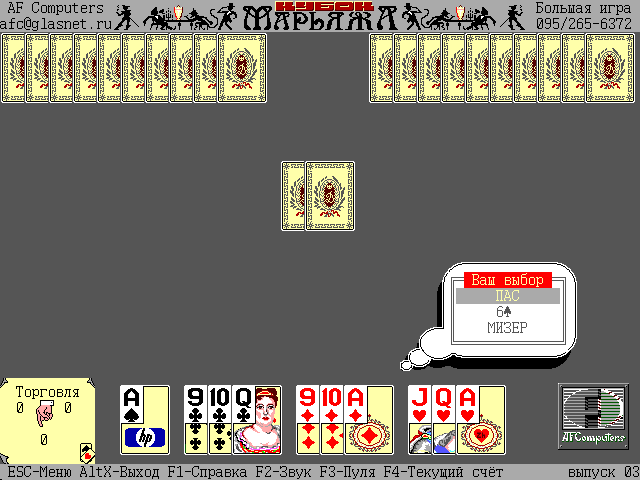
\includegraphics[scale=\FigScale]{examples/marriage/initial_not_patched.png}
\caption{"Торги"}
\end{figure}

Попробуем "подсмотреть" карты в "прикупе" в этой игре.

Для начала --- что мы знаем?
Игра под DOS, датируется 1997-м годом. IDA показывает имена стандартных функций вроде 
\TT{@GetImage\$q7Integert1t1t1m3Any} --- это "манглинг" типичный для Borland Pascal, что позволяет сделать вывод,
что сама игра написана на Паскале и скомпилирована Borland Pascal-ем.

Файлов около 10-и и некоторые имеют текстовую строку в заголовке "Marriage Image Library" --- вероятно,
это библиотеки спрайтов.

В IDA можно увидеть что используется функция \TT{@PutImage\$q7Integert1m3Any4Word}, которая, собственно,
рисует некий спрайт на экране.
Она вызывается по крайней мере из 8-и мест.
Чтобы узнать что происходит в каждом из этих 8-и мест, мы можем блокировать работу каждой функции и смотреть,
что будет происходить.
Например, первая ф-ция имеет адрес seg002:062E, и она заканчивается инструкцией \INS{retf 0Eh} на seg002:102A.
Это означает что метод вызовов ф-ций в Borland Pascal под DOS схож с stdcall --- вызываемая ф-ция должна сама
возвращать стек в состояние до того как началась передача аргументов.
В самом начале этой ф-ции вписываем инструкцию "retf 0eh", либо 3 байта: \TT{CA 0E 00}.
Запускаем "Марьяж" и внешне вроде бы ничего не изменилось.

Переходим ко второй ф-ции, которая активно использует \TT{@PutImage\$q7Integert1m3Any4Word}.
Она находится по адресу seg008:0AB5 и заканчивается инструкцией \INS{retf 0Ah}.
Вписываем эту инструкцию в самом начале и запускаем:

\begin{figure}[H]
\centering
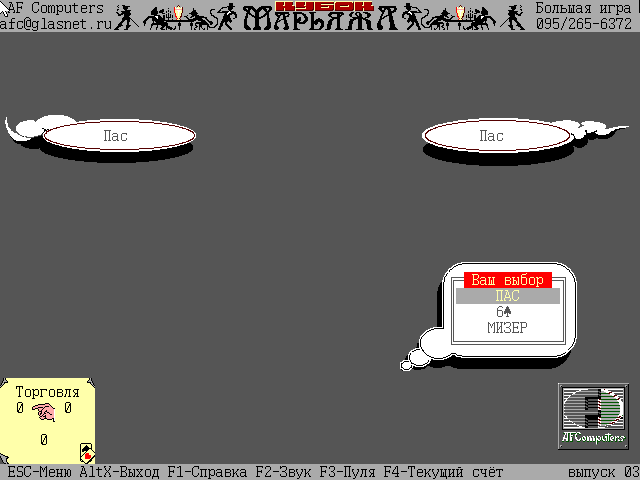
\includegraphics[scale=\FigScale]{examples/marriage/draw_card_bypass.png}
\caption{Карт нет}
\end{figure}

Карт не видно вообще. И видимо, эта функция их отображает, мы её заблокировали, и теперь карт не видно.
Назовем эту ф-цию в IDA \TT{draw\_card()}.
Помимо \TT{@PutImage\$q7Integert1m3Any4Word}, в этой ф-ции вызываются также ф-ции @SetColor\$q4Word, 
\TT{@SetFillStyle\$q4Wordt1}, \TT{@Bar\$q7Integert1t1t1}, \TT{@OutTextXY\$q7Integert16String}.

Сама ф-ция \TT{draw\_cards()} (её название мы дали ей сами только что) вызывается из 4-х мест.
Попробуем точно также "блокировать" каждую ф-цию.

Когда я "блокирую" вторую, по адресу seg008:0DF3 и запускаю программу, вижу такое:

\begin{figure}[H]
\centering
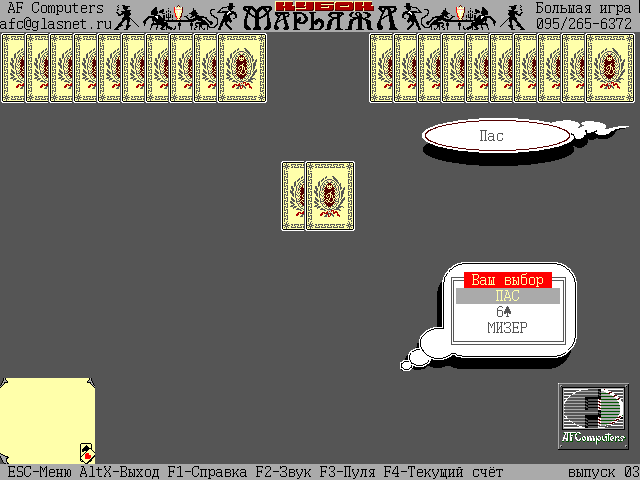
\includegraphics[scale=\FigScale]{examples/marriage/draw_players_cards.png}
\caption{Все карты кроме карт игрока}
\end{figure}

Видны все карты, кроме карт игрока. Видимо, эта функция рисует карты игрока. \\
Я переименовываю её в IDA в \TT{draw\_players\_cards()}.

Четвертая ф-ция, вызывающая \TT{draw\_cards()}, находится по адресу seg008:16B3, и когда я её "блокирую",
я вижу в игре такое:

\begin{figure}[H]
\centering
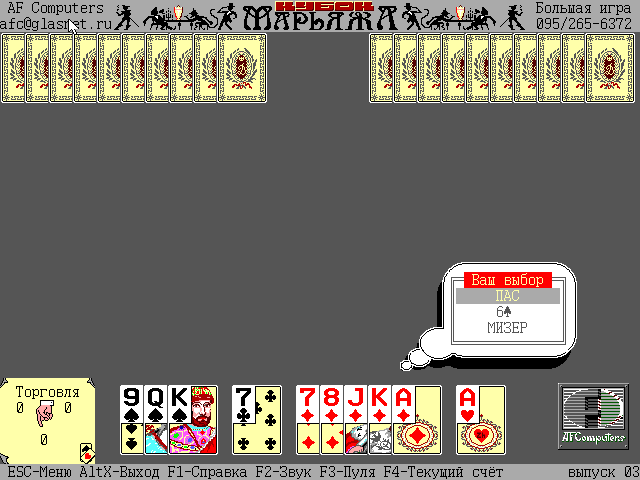
\includegraphics[scale=\FigScale]{examples/marriage/no_prikup.png}
\caption{"Прикупа" нет}
\end{figure}

Все карты есть, кроме "прикупа". Более того, эта ф-ция вызывает только \TT{draw\_cards()}, и только 2 раза.
Видимо эта ф-ция и отображает карты "прикупа".
Будем рассматривать её внимательнее.

\begin{lstlisting}
seg008:16B3 draw_prikup     proc far                ; CODE XREF: seg010:00B0
seg008:16B3                                         ; sub_15098+6
seg008:16B3
seg008:16B3 var_E           = word ptr -0Eh
seg008:16B3 var_C           = word ptr -0Ch
seg008:16B3 arg_0           = byte ptr  6
seg008:16B3
seg008:16B3                 enter   0Eh, 0
seg008:16B7                 mov     al, byte_2C0EA
seg008:16BA                 xor     ah, ah
seg008:16BC                 imul    ax, 23h
seg008:16BF                 mov     [bp+var_C], ax
seg008:16C2                 mov     al, byte_2C0EB
seg008:16C5                 xor     ah, ah
seg008:16C7                 imul    ax, 0Ah
seg008:16CA                 mov     [bp+var_E], ax
seg008:16CD                 cmp     [bp+arg_0], 0
seg008:16D1                 jnz     short loc_1334A
seg008:16D3                 cmp     byte_2BB08, 0
seg008:16D8                 jz      short loc_13356
seg008:16DA
seg008:16DA loc_1334A:                              ; CODE XREF: draw_prikup+1E
seg008:16DA                 mov     al, byte ptr word_32084
seg008:16DD                 mov     byte_293AD, al
seg008:16E0                 mov     al, byte ptr word_32086
seg008:16E3                 mov     byte_293AC, al
seg008:16E6
seg008:16E6 loc_13356:                              ; CODE XREF: draw_prikup+25
seg008:16E6                 mov     al, byte_293AC
seg008:16E9                 xor     ah, ah
seg008:16EB                 push    ax
seg008:16EC                 mov     al, byte_293AD
seg008:16EF                 xor     ah, ah
seg008:16F1                 push    ax
seg008:16F2                 push    [bp+var_C]
seg008:16F5                 push    [bp+var_E]
seg008:16F8                 cmp     [bp+arg_0], 0
seg008:16FC                 jnz     short loc_13379
seg008:16FE                 cmp     byte_2BB08, 0
seg008:1703                 jnz     short loc_13379
seg008:1705                 mov     al, 0
seg008:1707                 jmp     short loc_1337B
seg008:1709 ; ---------------------------------------------------------------------------
seg008:1709
seg008:1709 loc_13379:                              ; CODE XREF: draw_prikup+49
seg008:1709                                         ; draw_prikup+50
seg008:1709                 mov     al, 1
seg008:170B
seg008:170B loc_1337B:                              ; CODE XREF: draw_prikup+54
seg008:170B                 push    ax
seg008:170C                 push    cs
seg008:170D                 call    near ptr draw_card
seg008:1710                 mov     al, byte_2C0EA
seg008:1713                 xor     ah, ah
seg008:1715                 mov     si, ax
seg008:1717                 shl     ax, 1
seg008:1719                 add     ax, si
seg008:171B                 add     ax, [bp+var_C]
seg008:171E                 mov     [bp+var_C], ax
seg008:1721                 cmp     [bp+arg_0], 0
seg008:1725                 jnz     short loc_1339E
seg008:1727                 cmp     byte_2BB08, 0
seg008:172C                 jz      short loc_133AA
seg008:172E
seg008:172E loc_1339E:                              ; CODE XREF: draw_prikup+72
seg008:172E                 mov     al, byte ptr word_32088
seg008:1731                 mov     byte_293AD, al
seg008:1734                 mov     al, byte ptr word_3208A
seg008:1737                 mov     byte_293AC, al
seg008:173A
seg008:173A loc_133AA:                              ; CODE XREF: draw_prikup+79
seg008:173A                 mov     al, byte_293AC
seg008:173D                 xor     ah, ah
seg008:173F                 push    ax
seg008:1740                 mov     al, byte_293AD
seg008:1743                 xor     ah, ah
seg008:1745                 push    ax
seg008:1746                 push    [bp+var_C]
seg008:1749                 push    [bp+var_E]
seg008:174C                 cmp     [bp+arg_0], 0
seg008:1750                 jnz     short loc_133CD
seg008:1752                 cmp     byte_2BB08, 0
seg008:1757                 jnz     short loc_133CD
seg008:1759                 mov     al, 0
seg008:175B                 jmp     short loc_133CF
seg008:175D ; ---------------------------------------------------------------------------
seg008:175D
seg008:175D loc_133CD:                              ; CODE XREF: draw_prikup+9D
seg008:175D                                         ; draw_prikup+A4
seg008:175D                 mov     al, 1
seg008:175F
seg008:175F loc_133CF:                              ; CODE XREF: draw_prikup+A8
seg008:175F                 push    ax
seg008:1760                 push    cs
seg008:1761                 call    near ptr draw_card ; prikup #2
seg008:1764                 leave
seg008:1765                 retf    2
seg008:1765 draw_prikup     endp
\end{lstlisting}

Интересно посмотреть, как именно вызывается \TT{draw\_prikup()}. У нее только один аргумент.

Иногда она вызывается с аргументом 1:

\begin{lstlisting}
...
seg010:084C                 push    1
seg010:084E                 call    draw_prikup
...
\end{lstlisting}

А иногда с аргументом 0, причем вот в таком контексте, где уже есть другая знакомая функция:

\begin{lstlisting}
seg010:0067                 push    1
seg010:0069                 mov     al, byte_31F41
seg010:006C                 push    ax
seg010:006D                 call    sub_12FDC
seg010:0072                 push    1
seg010:0074                 mov     al, byte_31F41
seg010:0077                 push    ax
seg010:0078                 call    draw_players_cards
seg010:007D                 push    2
seg010:007F                 mov     al, byte_31F42
seg010:0082                 push    ax
seg010:0083                 call    sub_12FDC
seg010:0088                 push    2
seg010:008A                 mov     al, byte_31F42
seg010:008D                 push    ax
seg010:008E                 call    draw_players_cards
seg010:0093                 push    3
seg010:0095                 mov     al, byte_31F43
seg010:0098                 push    ax
seg010:0099                 call    sub_12FDC
seg010:009E                 push    3
seg010:00A0                 mov     al, byte_31F43
seg010:00A3                 push    ax
seg010:00A4                 call    draw_players_cards
seg010:00A9                 call    sub_1257A
seg010:00AE                 push    0
seg010:00B0                 call    draw_prikup
seg010:00B5                 mov     byte_2BB95, 0
\end{lstlisting}

Так что единственный аргумент у \TT{draw\_prikup()} может быть или 0 или 1, т.е., это, возможно, булевый тип.
На что он влияет внутри самой ф-ции?
При ближайшем рассмотрении видно, что входящий 0 или 1 передается в \TT{draw\_card()}, т.е., у последней тоже есть
булевый аргумент.
Помимо всего прочего, если передается 1, то по адресам seg008:16DA и seg008:172E копируются несколько байт
из одной группы глобальных переменных в другую.

Эксперимент: здесь 4 раза сравнивается единственный аргумент с 0 и далее следует \INS{JNZ}.
Что если сравнение будет происходит с 1, и, таким образом, работа функции \TT{draw\_prikup()} будет обратной?
Патчим и запускаем:

\begin{figure}[H]
\centering
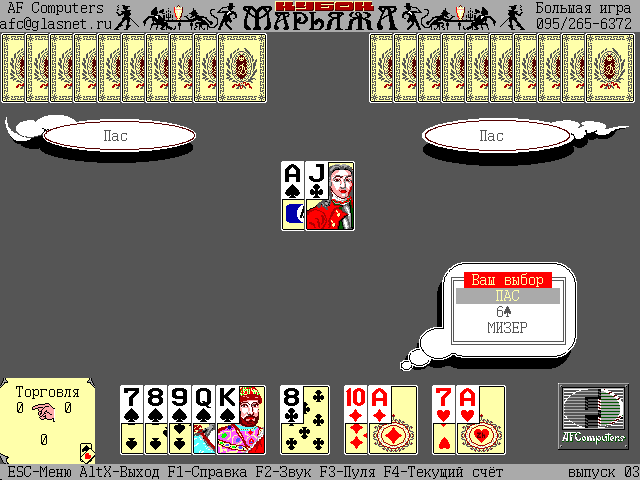
\includegraphics[scale=\FigScale]{examples/marriage/patch1.png}
\caption{"Прикуп" открыт}
\end{figure}

"Прикуп" открыт, но когда я делаю "заказ", и, по логике вещей, "прикуп" теперь должен стать открытым,
он наоборот становится закрытым:

\begin{figure}[H]
\centering
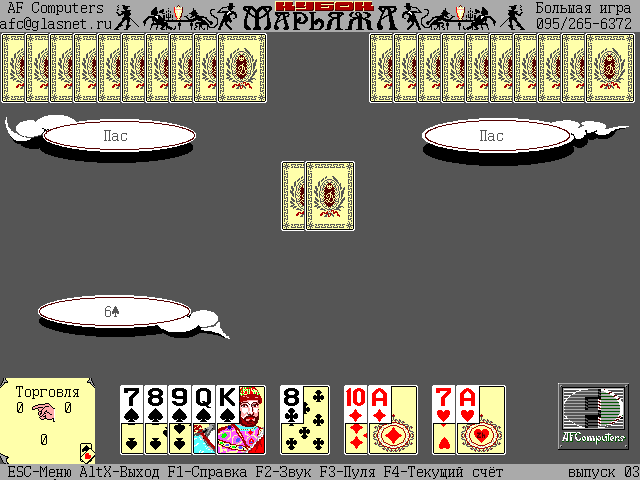
\includegraphics[scale=\FigScale]{examples/marriage/patch2.png}
\caption{"Прикуп" закрыт}
\end{figure}

Всё ясно: если аргумент \TT{draw\_prikup()} нулевой, то карты рисуются рубашкой вверх, если 1, то открытые.
Этот же аргумент передается в \TT{draw\_card()} --- эта ф-ция может рисовать и открытые и закрытые карты.

Пропатчить "Марьяж" теперь легко, достаточно исправить все условные переходы так, как будто бы в ф-цию
всегда приходит 1 в аргументе и тогда "прикуп" всегда будет открыт.

Но что за байты копируются в seg008:16DA и seg008:172E?
Я попробовал забить инструкции копирования \MOV \NOP{}-ами --- "прикуп" вообще перестал отображаться.

Тогда я сделал так, чтобы всегда записывалась 1:

\begin{lstlisting}
...
00004B5A: B001                           mov         al,1
00004B5C: 90                             nop
00004B5D: A26D08                         mov         [0086D],al
00004B60: B001                           mov         al,1
00004B62: 90                             nop
00004B63: A26C08                         mov         [0086C],al
...
\end{lstlisting}

Тогда "прикуп" отображается как два пиковых туза.
А если первый байт --- 2, а второй --- 1, получается трефовый туз.
Видимо так и кодируется масть карты, а затем и сама карта.
% TODO \ref{} сюда о том, как можно передавать аргументы в глоб.переменных
А \TT{draw\_card()} затем считывает эту информацию из пары глобальных переменных.
А копируется она тоже из глобальных переменных, где собственно и находится состояние карт у игроков и в прикупе
после случайной тасовки.
Но нельзя забывать что если мы сделаем так, что в "прикупе" всегда будет 2 пиковых туза, это будет только
на экране так отображаться, а в памяти состояние карт останется таким же, как и после тасовки.

Я также пробовал сделать пранк: во время торгов одна карта "прикупа" открыта, а вторая закрыта, а после "заказа",
наоборот, первая закрыта, а вторая открывается. В качестве упражнения, вы можете попробовать сделать так.

Еще кое-что: чтобы сделать прикуп открытым, ведь можно же найти место где вызывается \TT{draw\_prikup()} и поменять 0
на 1. Можно, только это место не в головой marriage.exe, а в marriage.000, а это DOS-овский оверлей (начинается
с сигнатуры "FBOV").

В качестве упражнения, можно попробовать подсматривать состояние всех карт, и у обоих игроков.
Для этого нужно отладчиком смотреть состояние глобальной памяти рядом с тем, откуда считываются обе карты
прикупа.

Файлы: \\
оригинальная версия: \url{http://beginners.re/examples/marriage/original.zip}, \\
пропатченная мною версия: \url{http://beginners.re/examples/marriage/patched.zip} 
(все 4 условных перехода после \TT{cmp [bp+arg\_0], 0} заменены на \JMP).

}

\renewcommand{\CURPATH}{advanced/102_fib}
\chapter{\RU{Конверсия строки в число}\EN{String to number conversion} (atoi())}

\myindex{\CStandardLibrary!atoi()}
\RU{Попробуем реализовать стандарту функцию Си atoi().}
\EN{Let's try to reimplement the standard atoi() C function.}

\section{\RU{Простой пример}\EN{Simple example}}

\RU{Это самый простой способ прочитать число, представленное в кодировке \ac{ASCII}.}
\EN{Here is the simplest possible way to read a number represented in \ac{ASCII} encoding.}
\RU{Он не защищен от ошибок: символ отличный от цифры приведет к неверному результату.}
\EN{It's not error-prone: a character other than a digit leads to incorrect result.}

\lstinputlisting{\CURPATH/atoi.c}

\RU{То, что делает алгоритм это просто считывает цифры слева направо.}
\EN{So what the algorithm does is just reading digits from left to right.}
\RU{Символ нуля в \ac{ASCII} вычитается из каждой цифры.}
\EN{The zero \ac{ASCII} character is subtracted from each digit. }
\RU{Цифры от \q{0} до \q{9} расположены по порядку в таблице \ac{ASCII}, так что мы даже можем
и не знать точного значения символа \q{0}.}
\EN{The digits from \q{0} to \q{9} are consecutive in the \ac{ASCII} table, so 
we do not even need to know the exact value of the \q{0} character.}
\RU{Всё что нам нужно знать это то что \q{0} минус \q{0}\EMDASH{}это 0, а \q{9} минус \q{0} это 9, \etc{}.}
\EN{All we need to know is that \q{0} minus \q{0} is 0, \q{9} minus \q{0}'is 9 and so on.}
\RU{Вычитание \q{0} от каждого символа в итоге дает число от 0 до 9 включительно.}
\EN{Subtracting \q{0} from each character results in a number from 0 to 9 inclusive.}
\RU{Любой другой символ, конечно, приведет к неверному результату!}
\EN{Any other character leads to an incorrect result, of course!}
\RU{Каждая цифра добавляется к итоговому результату (в переменной \q{rt}), но итоговый результат
также умножается на 10 на каждой цифре.}
\EN{Each digit has to be added to the final result (in variable \q{rt}), but the final result
is also multiplied by 10 at each digit.}
\RU{Другими словами, на каждой итерации, результат сдвигается влево на одну позицию в десятичном виде.}
\EN{In other words, the result is shifted left by one position in decimal form on each iteration.}
\RU{Самая последняя цифра прибавляется, но не сдвигается.}
\EN{The last digit is added, but there is no no shift.}

\subsection{\Optimizing MSVC 2013 x64}

\lstinputlisting[caption=\Optimizing MSVC 2013 x64]{\CURPATH/atoi.asm.MSVC2013.x64.Ox.\LANG}

\RU{Символы загружаются в двух местах: первый символ и все последующие символы.}
\EN{A character can be loaded in two places: the first character and all subsequent characters.}
\RU{Это сделано для перегруппировки цикла.}\EN{This is done for loop regrouping.}
\myindex{x86!\Instructions!LEA}
\RU{Здесь нет инструкции для умножения на 10, вместо этого две LEA делают это же.}
\EN{There is no instruction for multiplication by 10, two LEA instruction do this instead.}
\myindex{x86!\Instructions!ADD}
\myindex{x86!\Instructions!SUB}
\RU{MSVC иногда использует инструкцию ADD с отрицательной константой вместо SUB.}
\EN{MSVC sometimes uses the ADD instruction with a negative constant instead of SUB.}
\RU{Это тот случай}\EN{This is the case}.
\RU{Честно говоря, трудно сказать, чем это лучше, чем SUB.}
\EN{It's very hard to say why this is better then SUB.}
\RU{Но MSVC делает так часто}\EN{But MSVC does this often}.

\subsection{\Optimizing GCC 4.9.1 x64}

\Optimizing GCC 4.9.1 \RU{более краток, но здесь есть одна лишняя инструкция RET в конце.}
\EN{is more concise, but there is one redundant RET instruction at the end.}
\RU{Одной было бы достаточно}\EN{One would be enough}.

\lstinputlisting[caption=\Optimizing GCC 4.9.1 x64]{\CURPATH/atoi.s.GCC491.O3.x64.\LANG}

\subsection{\OptimizingKeilVI (\ARMMode)}

\lstinputlisting[caption=\OptimizingKeilVI (\ARMMode)]{\CURPATH/atoi.s.ARM.O3.\LANG}

\subsection{\OptimizingKeilVI (\ThumbMode)}

\lstinputlisting[caption=\OptimizingKeilVI (\ThumbMode)]{\CURPATH/atoi.s.thumb.O3.\LANG}

\RU{Интересно, из школьного курса математики мы можем помнить что порядок операций сложения и вычитания
не играет роли.}
\EN{Interestingly, from school mathematics we may remember that the order of addition and 
subtraction operations doesn't matter.}
\RU{Это наш случай: в начале вычисляется выражение $rt*10 - '0'$, затем к нему прибавляется 
значение входного символа.}
\EN{That's our case: first, the $rt*10 - '0'$ expression is computed, then the input character value 
is added to it.}
\RU{Действительно, результат тот же, но компилятор немного всё перегруппировал.}
\EN{Indeed, the result is the same, but the compiler did some regrouping.}

\subsection{\Optimizing GCC 4.9.1 ARM64}

\RU{Компилятор для ARM64 может использовать суффикс инструкции, задающий пре-инкремент:}
\EN{The ARM64 compiler can use the pre-increment instruction suffix:}

\lstinputlisting[caption=\Optimizing GCC 4.9.1 ARM64]{\CURPATH/atoi.s.GCC49.ARM64.O3.\LANG}

\section{\RU{Немного расширенный пример}\EN{A slightly advanced example}}

\RU{Новый пример более расширенный, теперь здесь есть проверка знака \q{минус} в самом начале,
и еще он может сообщать об ошибке если не-цифра была найдена во входной строке:}
\EN{My new code snippet is more advanced, now it checks for the \q{minus} sign at the first character
and reports an error if a non-digit was found in the input string:}

\lstinputlisting{\CURPATH/atoi2.c}

\subsection{\Optimizing GCC 4.9.1 x64}

\lstinputlisting[caption=\Optimizing GCC 4.9.1 x64]{\CURPATH/atoi2.s.GCC491.O3.x64.\LANG}

\myindex{x86!\Instructions!NEG}
\RU{Если знак \q{минус} был найден в начале строки, инструкция NEG будет исполнена в конце.}
\EN{If the \q{minus} sign was encountered at the string start, the NEG instruction is to be executed at the end.}
\RU{Она просто меняет знак числа}\EN{It just negates the number}.

\label{one_comparison_instead_of_two}
\RU{Еще кое-что надо отметить}\EN{There is one more thing that needs mentioning}.
\RU{Как среднестатистический программист будет проверять, является ли символ цифрой?}
\EN{How would a common programmer check if the character is not a digit?}
\RU{Так же, как и у нас в исходном коде}\EN{Just how we have it in the source code}:

\begin{lstlisting}
if (*s<'0' || *s>'9')
    ...
\end{lstlisting}

\RU{Здесь две операции сравнения}\EN{There are two comparison operations}.
\RU{Но что интересно, так это то что мы можем заменить обе операции на одну:}
\EN{What is interesting is that we can replace both operations by single one:}
\RU{просто вычитайте \q{0} из значения символа}\EN{just subtract \q{0} from character value},
\RU{считается результат за беззнаковое значение (это важно) и проверьте, не больше ли он чем 9.}
\EN{treat result as unsigned value (this is important) and check if it's greater than 9.}

\RU{Например, скажем, строка на входе имеет символ точки (\q{.}), которая имеет код 46 в таблице \ac{ASCII}.}
\EN{For example, let's say that the user input contains the dot character (\q{.}) which has \ac{ASCII} code 46.}
$46-48=-2$ \RU{если считать результат за знаковое число}\EN{if we treat the result as a signed number}.
\RU{Действительно, символ точки расположен на два места раньше, чем символ \q{0} в таблице \ac{ASCII}.}
\EN{Indeed, the dot character is located two places earlier than the \q{0} character in the \ac{ASCII} table.}
\RU{Но это}\EN{But it is} \TT{0xFFFFFFFE} (4294967294) \RU{если считать результат за беззнаковое значение, 
и это точно больше чем 9!}
\EN{if we treat the result as an unsigned value, and that's definitely bigger than 9!}

\RU{Компиляторы часто так делают, важно распознавать эти трюки.}
\EN{The compilers do this often, so it's important to recognize these tricks.}

\EN{Another example of it in this book}\RU{Еще один пример подобного в этой книге}: 
\myref{toupper_one_comparison}.

\Optimizing MSVC 2013 x64 \RU{применяет те же трюки}\EN{does the same tricks}.

\subsection{\OptimizingKeilVI (\ARMMode)}

\lstinputlisting[caption=\OptimizingKeilVI (\ARMMode),numbers=left]{\CURPATH/atoi2.s.ARM.O3.\LANG}

\RU{В 32-битном ARM нет инструкции NEG, так что вместо этого используется операция \q{Reverse Subtraction}
(строка 31).}
\EN{There is no NEG instruction in 32-bit ARM, so the \q{Reverse Subtraction} operation (line 31) 
is used here.}
\RU{Она сработает если результат инструкции CMP (на строке 29) был \q{Not Equal} 
(не равно, отсюда суффикс -NE suffix).}
\EN{It is triggered if the result of the CMP instruction (at line 29) was \q{Not Equal} (hence -NE suffix).}
\myindex{ARM!\Instructions!RSB}
\RU{Что делает RSBNE это просто вычитает результирующее значение из нуля.}
\EN{So what RSBNE does is to subtract the resulting value from 0.}
\RU{Она работает, как и обычное вычитание, но меняет местами операнды.}
\EN{It works just like the regular subtraction operation, but swaps operands.}
\RU{Вычитание любого числа из нуля это смена знака}
\EN{Subtracting any number from 0 results in negation}: $0-x=-x$.

\RU{Код для режима Thumb почти такой же.}
\EN{Thumb mode code is mostly the same.}

\myindex{ARM!\Instructions!NEG}
GCC 4.9 \ForENRU ARM64 \RU{может использовать инструкцию NEG, доступную в}
\EN{can use the NEG instruction, which is available in} ARM64.

\section{\Exercise{}}

\myindex{Fuzzing}
\EN{Oh, by the way, security researchers deals often with unpredictable behaviour of program while handling of incorrect data.}
\RU{Кстати, security research-еры часто имеют дело с непредсказуемым поведением программ во время обработки некорректных данных.}
\RU{Например, во время fuzzing-а.}
\EN{For example, while fuzzing.}
\EN{As an exercise, you may try to enter non-digit characters and see what happens.}
\RU{В качестве упражнения, вы можете попробовать ввести символы не относящиеся к числам и посмотреть, что случится.}
\EN{Try to explain, what happened and why.}
\RU{Попробуйте объяснить, что произошло, и почему.}




\renewcommand{\CURPATH}{advanced/110_CRC32}
\chapter{\RU{Конверсия строки в число}\EN{String to number conversion} (atoi())}

\myindex{\CStandardLibrary!atoi()}
\RU{Попробуем реализовать стандарту функцию Си atoi().}
\EN{Let's try to reimplement the standard atoi() C function.}

\section{\RU{Простой пример}\EN{Simple example}}

\RU{Это самый простой способ прочитать число, представленное в кодировке \ac{ASCII}.}
\EN{Here is the simplest possible way to read a number represented in \ac{ASCII} encoding.}
\RU{Он не защищен от ошибок: символ отличный от цифры приведет к неверному результату.}
\EN{It's not error-prone: a character other than a digit leads to incorrect result.}

\lstinputlisting{\CURPATH/atoi.c}

\RU{То, что делает алгоритм это просто считывает цифры слева направо.}
\EN{So what the algorithm does is just reading digits from left to right.}
\RU{Символ нуля в \ac{ASCII} вычитается из каждой цифры.}
\EN{The zero \ac{ASCII} character is subtracted from each digit. }
\RU{Цифры от \q{0} до \q{9} расположены по порядку в таблице \ac{ASCII}, так что мы даже можем
и не знать точного значения символа \q{0}.}
\EN{The digits from \q{0} to \q{9} are consecutive in the \ac{ASCII} table, so 
we do not even need to know the exact value of the \q{0} character.}
\RU{Всё что нам нужно знать это то что \q{0} минус \q{0}\EMDASH{}это 0, а \q{9} минус \q{0} это 9, \etc{}.}
\EN{All we need to know is that \q{0} minus \q{0} is 0, \q{9} minus \q{0}'is 9 and so on.}
\RU{Вычитание \q{0} от каждого символа в итоге дает число от 0 до 9 включительно.}
\EN{Subtracting \q{0} from each character results in a number from 0 to 9 inclusive.}
\RU{Любой другой символ, конечно, приведет к неверному результату!}
\EN{Any other character leads to an incorrect result, of course!}
\RU{Каждая цифра добавляется к итоговому результату (в переменной \q{rt}), но итоговый результат
также умножается на 10 на каждой цифре.}
\EN{Each digit has to be added to the final result (in variable \q{rt}), but the final result
is also multiplied by 10 at each digit.}
\RU{Другими словами, на каждой итерации, результат сдвигается влево на одну позицию в десятичном виде.}
\EN{In other words, the result is shifted left by one position in decimal form on each iteration.}
\RU{Самая последняя цифра прибавляется, но не сдвигается.}
\EN{The last digit is added, but there is no no shift.}

\subsection{\Optimizing MSVC 2013 x64}

\lstinputlisting[caption=\Optimizing MSVC 2013 x64]{\CURPATH/atoi.asm.MSVC2013.x64.Ox.\LANG}

\RU{Символы загружаются в двух местах: первый символ и все последующие символы.}
\EN{A character can be loaded in two places: the first character and all subsequent characters.}
\RU{Это сделано для перегруппировки цикла.}\EN{This is done for loop regrouping.}
\myindex{x86!\Instructions!LEA}
\RU{Здесь нет инструкции для умножения на 10, вместо этого две LEA делают это же.}
\EN{There is no instruction for multiplication by 10, two LEA instruction do this instead.}
\myindex{x86!\Instructions!ADD}
\myindex{x86!\Instructions!SUB}
\RU{MSVC иногда использует инструкцию ADD с отрицательной константой вместо SUB.}
\EN{MSVC sometimes uses the ADD instruction with a negative constant instead of SUB.}
\RU{Это тот случай}\EN{This is the case}.
\RU{Честно говоря, трудно сказать, чем это лучше, чем SUB.}
\EN{It's very hard to say why this is better then SUB.}
\RU{Но MSVC делает так часто}\EN{But MSVC does this often}.

\subsection{\Optimizing GCC 4.9.1 x64}

\Optimizing GCC 4.9.1 \RU{более краток, но здесь есть одна лишняя инструкция RET в конце.}
\EN{is more concise, but there is one redundant RET instruction at the end.}
\RU{Одной было бы достаточно}\EN{One would be enough}.

\lstinputlisting[caption=\Optimizing GCC 4.9.1 x64]{\CURPATH/atoi.s.GCC491.O3.x64.\LANG}

\subsection{\OptimizingKeilVI (\ARMMode)}

\lstinputlisting[caption=\OptimizingKeilVI (\ARMMode)]{\CURPATH/atoi.s.ARM.O3.\LANG}

\subsection{\OptimizingKeilVI (\ThumbMode)}

\lstinputlisting[caption=\OptimizingKeilVI (\ThumbMode)]{\CURPATH/atoi.s.thumb.O3.\LANG}

\RU{Интересно, из школьного курса математики мы можем помнить что порядок операций сложения и вычитания
не играет роли.}
\EN{Interestingly, from school mathematics we may remember that the order of addition and 
subtraction operations doesn't matter.}
\RU{Это наш случай: в начале вычисляется выражение $rt*10 - '0'$, затем к нему прибавляется 
значение входного символа.}
\EN{That's our case: first, the $rt*10 - '0'$ expression is computed, then the input character value 
is added to it.}
\RU{Действительно, результат тот же, но компилятор немного всё перегруппировал.}
\EN{Indeed, the result is the same, but the compiler did some regrouping.}

\subsection{\Optimizing GCC 4.9.1 ARM64}

\RU{Компилятор для ARM64 может использовать суффикс инструкции, задающий пре-инкремент:}
\EN{The ARM64 compiler can use the pre-increment instruction suffix:}

\lstinputlisting[caption=\Optimizing GCC 4.9.1 ARM64]{\CURPATH/atoi.s.GCC49.ARM64.O3.\LANG}

\section{\RU{Немного расширенный пример}\EN{A slightly advanced example}}

\RU{Новый пример более расширенный, теперь здесь есть проверка знака \q{минус} в самом начале,
и еще он может сообщать об ошибке если не-цифра была найдена во входной строке:}
\EN{My new code snippet is more advanced, now it checks for the \q{minus} sign at the first character
and reports an error if a non-digit was found in the input string:}

\lstinputlisting{\CURPATH/atoi2.c}

\subsection{\Optimizing GCC 4.9.1 x64}

\lstinputlisting[caption=\Optimizing GCC 4.9.1 x64]{\CURPATH/atoi2.s.GCC491.O3.x64.\LANG}

\myindex{x86!\Instructions!NEG}
\RU{Если знак \q{минус} был найден в начале строки, инструкция NEG будет исполнена в конце.}
\EN{If the \q{minus} sign was encountered at the string start, the NEG instruction is to be executed at the end.}
\RU{Она просто меняет знак числа}\EN{It just negates the number}.

\label{one_comparison_instead_of_two}
\RU{Еще кое-что надо отметить}\EN{There is one more thing that needs mentioning}.
\RU{Как среднестатистический программист будет проверять, является ли символ цифрой?}
\EN{How would a common programmer check if the character is not a digit?}
\RU{Так же, как и у нас в исходном коде}\EN{Just how we have it in the source code}:

\begin{lstlisting}
if (*s<'0' || *s>'9')
    ...
\end{lstlisting}

\RU{Здесь две операции сравнения}\EN{There are two comparison operations}.
\RU{Но что интересно, так это то что мы можем заменить обе операции на одну:}
\EN{What is interesting is that we can replace both operations by single one:}
\RU{просто вычитайте \q{0} из значения символа}\EN{just subtract \q{0} from character value},
\RU{считается результат за беззнаковое значение (это важно) и проверьте, не больше ли он чем 9.}
\EN{treat result as unsigned value (this is important) and check if it's greater than 9.}

\RU{Например, скажем, строка на входе имеет символ точки (\q{.}), которая имеет код 46 в таблице \ac{ASCII}.}
\EN{For example, let's say that the user input contains the dot character (\q{.}) which has \ac{ASCII} code 46.}
$46-48=-2$ \RU{если считать результат за знаковое число}\EN{if we treat the result as a signed number}.
\RU{Действительно, символ точки расположен на два места раньше, чем символ \q{0} в таблице \ac{ASCII}.}
\EN{Indeed, the dot character is located two places earlier than the \q{0} character in the \ac{ASCII} table.}
\RU{Но это}\EN{But it is} \TT{0xFFFFFFFE} (4294967294) \RU{если считать результат за беззнаковое значение, 
и это точно больше чем 9!}
\EN{if we treat the result as an unsigned value, and that's definitely bigger than 9!}

\RU{Компиляторы часто так делают, важно распознавать эти трюки.}
\EN{The compilers do this often, so it's important to recognize these tricks.}

\EN{Another example of it in this book}\RU{Еще один пример подобного в этой книге}: 
\myref{toupper_one_comparison}.

\Optimizing MSVC 2013 x64 \RU{применяет те же трюки}\EN{does the same tricks}.

\subsection{\OptimizingKeilVI (\ARMMode)}

\lstinputlisting[caption=\OptimizingKeilVI (\ARMMode),numbers=left]{\CURPATH/atoi2.s.ARM.O3.\LANG}

\RU{В 32-битном ARM нет инструкции NEG, так что вместо этого используется операция \q{Reverse Subtraction}
(строка 31).}
\EN{There is no NEG instruction in 32-bit ARM, so the \q{Reverse Subtraction} operation (line 31) 
is used here.}
\RU{Она сработает если результат инструкции CMP (на строке 29) был \q{Not Equal} 
(не равно, отсюда суффикс -NE suffix).}
\EN{It is triggered if the result of the CMP instruction (at line 29) was \q{Not Equal} (hence -NE suffix).}
\myindex{ARM!\Instructions!RSB}
\RU{Что делает RSBNE это просто вычитает результирующее значение из нуля.}
\EN{So what RSBNE does is to subtract the resulting value from 0.}
\RU{Она работает, как и обычное вычитание, но меняет местами операнды.}
\EN{It works just like the regular subtraction operation, but swaps operands.}
\RU{Вычитание любого числа из нуля это смена знака}
\EN{Subtracting any number from 0 results in negation}: $0-x=-x$.

\RU{Код для режима Thumb почти такой же.}
\EN{Thumb mode code is mostly the same.}

\myindex{ARM!\Instructions!NEG}
GCC 4.9 \ForENRU ARM64 \RU{может использовать инструкцию NEG, доступную в}
\EN{can use the NEG instruction, which is available in} ARM64.

\section{\Exercise{}}

\myindex{Fuzzing}
\EN{Oh, by the way, security researchers deals often with unpredictable behaviour of program while handling of incorrect data.}
\RU{Кстати, security research-еры часто имеют дело с непредсказуемым поведением программ во время обработки некорректных данных.}
\RU{Например, во время fuzzing-а.}
\EN{For example, while fuzzing.}
\EN{As an exercise, you may try to enter non-digit characters and see what happens.}
\RU{В качестве упражнения, вы можете попробовать ввести символы не относящиеся к числам и посмотреть, что случится.}
\EN{Try to explain, what happened and why.}
\RU{Попробуйте объяснить, что произошло, и почему.}




\renewcommand{\CURPATH}{advanced/111_netmask}
\EN{\section{Text strings}

\subsection{\CCpp}

\label{C_strings}
The normal C strings are zero-terminated (\ac{ASCIIZ}-strings).

The reason why the C string format is as it is (zero-terminated) is apparently historical.
In [Dennis M. Ritchie, \IT{The Evolution of the Unix Time-sharing System}, (1979)]
we read:

\begin{framed}
\begin{quotation}
A minor difference was that the unit of I/O was the word, not the byte, because the PDP-7 was a word-addressed
machine. In practice this meant merely that all programs dealing with character streams ignored null
characters, because null was used to pad a file to an even number of characters.
\end{quotation}
\end{framed}

\myindex{Hiew}

In Hiew or FAR Manager these strings looks like this:

\begin{lstlisting}
int main()
{
	printf ("Hello, world!\n");
};
\end{lstlisting}

\begin{figure}[H]
\centering
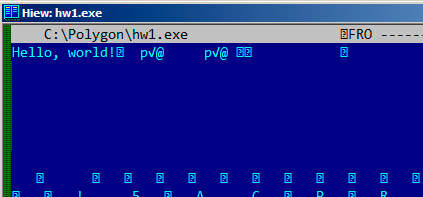
\includegraphics[scale=\NormalScale]{digging_into_code/strings/C-string.png}
\caption{Hiew}
\end{figure}

% FIXME видно \n в конце, потом пробел

\subsection{Borland Delphi}
\myindex{Pascal}
\myindex{Borland Delphi}

The string in Pascal and Borland Delphi is preceded by an 8-bit or 32-bit string length.

For example:

\begin{lstlisting}[caption=Delphi]
CODE:00518AC8                 dd 19h
CODE:00518ACC aLoading___Plea db 'Loading... , please wait.',0

...

CODE:00518AFC                 dd 10h
CODE:00518B00 aPreparingRun__ db 'Preparing run...',0
\end{lstlisting}

\subsection{Unicode}

\myindex{Unicode}

Often, what is called Unicode is a methods for encoding strings where each character occupies 2 bytes or 16 bits.
This is a common terminological mistake.
Unicode is a standard for assigning a number to each character in the many writing systems of the 
world, but does not describe the encoding method.

\myindex{UTF-8}
\myindex{UTF-16LE}
The most popular encoding methods are: UTF-8 (is widespread in Internet and *NIX systems) and UTF-16LE (is used in Windows).

\subsubsection{UTF-8}

\myindex{UTF-8}
UTF-8 is one of the most successful methods for
encoding characters.
All Latin symbols are encoded just like in ASCII,
and the symbols beyond the ASCII table are encoded using several bytes.
0 is encoded as
before, so all standard C string functions work with UTF-8 strings just like any other string.

Let's see how the symbols in various languages are encoded in UTF-8 and how it looks like in FAR, using the 437 codepage
\footnote{The example and translations was taken from here: 
\url{http://go.yurichev.com/17304}}:

\begin{figure}[H]
\centering

\includegraphics[scale=\NormalScale]{digging_into_code/strings/multilang_sampler.png}
\end{figure}

% FIXME: cut it
\begin{figure}[H]
\centering
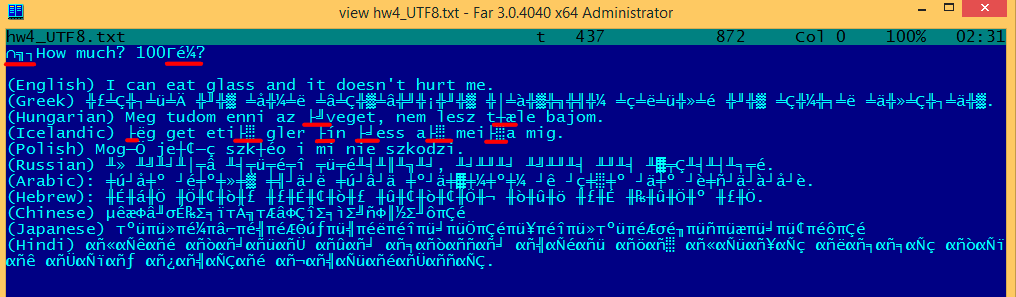
\includegraphics[scale=\FigScale]{digging_into_code/strings/multilang_sampler_UTF8.png}
\caption{FAR: UTF-8}
\end{figure}

As you can see, the English language string looks the same as it is in ASCII.

The Hungarian language uses some Latin symbols plus symbols with diacritic marks.

These symbols are encoded using several bytes, these are underscored with red.
It's the same story with the Icelandic and Polish languages.

There is also the \q{Euro} currency symbol at the start, which is encoded with 3 bytes.

The rest of the writing systems here have no connection with Latin.

At least in Russian, Arabic, Hebrew and Hindi we can see some recurring bytes, and that is not surprise:
all symbols from a writing system are usually located in the same Unicode table, so their code begins with
the same numbers.

At the beginning, before the \q{How much?} string we see 3 bytes, which are in fact the \ac{BOM}.
The \ac{BOM} defines the encoding system to be
used.

\subsubsection{UTF-16LE}

\myindex{UTF-16LE}
\myindex{Windows!Win32}
Many win32 functions in Windows have the suffixes \TT{-A} and \TT{-W}.
The first type of functions works
with normal strings, the other with UTF-16LE strings (\IT{wide}).

In the second case, each symbol is usually stored in a 16-bit value of type \IT{short}.

The Latin symbols in UTF-16 strings look in Hiew or FAR like they are interleaved with zero byte:

\begin{lstlisting}
int wmain()
{
	wprintf (L"Hello, world!\n");
};
\end{lstlisting}

\begin{figure}[H]
\centering
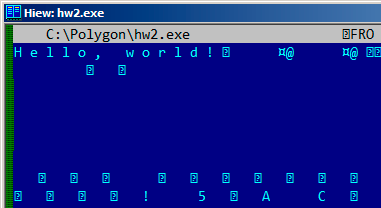
\includegraphics[scale=\NormalScale]{digging_into_code/strings/UTF16-string.png}
\caption{Hiew}
\end{figure}

We can see this often in \gls{Windows NT} system files:

\begin{figure}[H]
\centering
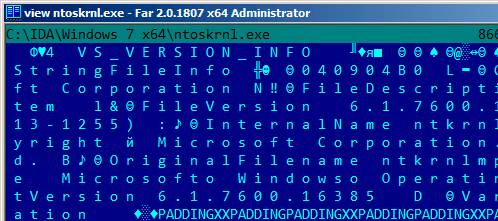
\includegraphics[scale=\NormalScale]{digging_into_code/strings/ntoskrnl_UTF16.png}
\caption{Hiew}
\end{figure}

\myindex{IDA}
Strings with characters that occupy exactly 2 bytes are called \q{Unicode} in \IDA:

\begin{lstlisting}
.data:0040E000 aHelloWorld:
.data:0040E000                 unicode 0, <Hello, world!>
.data:0040E000                 dw 0Ah, 0
\end{lstlisting}

Here is how the Russian language string is encoded in UTF-16LE:

\begin{figure}[H]
\centering
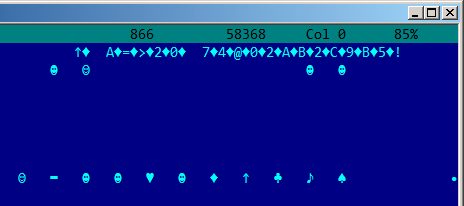
\includegraphics[scale=\NormalScale]{digging_into_code/strings/russian_UTF16.png}
\caption{Hiew: UTF-16LE}
\end{figure}

What we can easily spot is that the symbols are interleaved by the diamond character (which has the ASCII code of 4).
Indeed, the Cyrillic symbols are located in the fourth Unicode plane
\footnote{\href{http://go.yurichev.com/17003}{wikipedia}}.
Hence, all Cyrillic symbols in UTF-16LE are located in the \TT{0x400-0x4FF} range.

Let's go back to the example with the string written in multiple languages.
Here is how it looks like in UTF-16LE.

% FIXME: cut it
\begin{figure}[H]
\centering
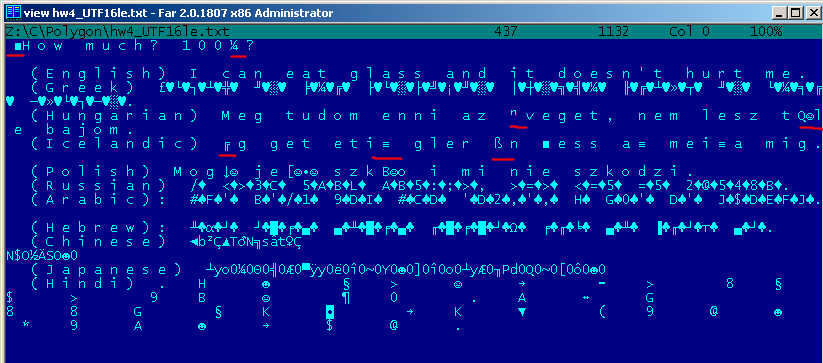
\includegraphics[scale=\FigScale]{digging_into_code/strings/multilang_sampler_UTF16.png}
\caption{FAR: UTF-16LE}
\end{figure}

Here we can also see the \ac{BOM} in the beginning.
All Latin characters are interleaved with a zero byte.

Some characters with diacritic marks (Hungarian and Icelandic languages) are also underscored in red.

% TODO: strings *NIX utility. procmonitor also shows strings...

% subsection:
\subsection{Base64}
\myindex{Base64}

The base64 encoding is highly popular for the cases when you need to transfer binary data as a text string.

In essence, this algorithm encodes 3 binary bytes into 4 printable characters:
all 26 Latin letters (both lower and upper case), digits, plus sign (\q{+}) and slash sign (\q{/}),
64 characters in total.

One distinctive feature of base64 strings is that they often (but not always) ends with 1 or 2 \gls{padding}
equality symbol(s) (\q{=}), for example:

\begin{lstlisting}
AVjbbVSVfcUMu1xvjaMgjNtueRwBbxnyJw8dpGnLW8ZW8aKG3v4Y0icuQT+qEJAp9lAOuWs=
\end{lstlisting}

\begin{lstlisting}
WVjbbVSVfcUMu1xvjaMgjNtueRwBbxnyJw8dpGnLW8ZW8aKG3v4Y0icuQT+qEJAp9lAOuQ==
\end{lstlisting}

The equality sign (\q{=}) is never encounter in the middle of base64-encoded strings.

Now example of manual encoding.
Let's encode 0x00, 0x11, 0x22, 0x33 hexadecimal bytes into base64 string:

\lstinputlisting{digging_into_code/strings/base64_ex.sh}

Let's put all 4 bytes in binary form, then regroup them into 6-bit groups:

\begin{lstlisting}
|  00  ||  11  ||  22  ||  33  ||      ||      |
00000000000100010010001000110011????????????????
| A  || B  || E  || i  || M  || w  || =  || =  |
\end{lstlisting}

Three first bytes (0x00, 0x11, 0x22) can be encoded into 4 base64 characters (``ABEi''),
but the last one (0x33) --- cannot be,
so it's encoded using two characters (``Mw'') and \gls{padding} symbol (``='')
is added twice to pad the last group to 4 characters.
Hence, length of all correct base64 strings are always divisible by 4.

\myindex{XML}
Base64 is often used when binary data needs to be stored in XML.

Some people tries to use base64 to obfuscate strings:
\url{http://blog.sec-consult.com/2016/01/deliberately-hidden-backdoor-account-in.html}
\footnote{\url{http://archive.is/nDCas}}.

\myindex{base64scanner}
There are utilities for scanning an arbitrary binary files for base64 strings.
One such utilitiy is base64scanner\footnote{\url{https://github.com/dennis714/base64scanner}}.

\myindex{UseNet}
\myindex{FidoNet}
\myindex{Uuencoding}
Another encoding system which was much more popular in UseNet and FidoNet is Uuencoding.
It offers mostly the same features, but is different from base64 in the sense that file name
is also stored in header.


}
\RU{\chapter{"Прикуп" в игре "Марьяж"}

\epigraph{Знал бы прикуп --- жил бы в Сочи.}{Поговорка.}

"Марьяж" --- старая и довольно популярная версия игры в "Преферанс" под DOS.

Играют три игрока, каждому раздается по 10 карт, остальные 2 остается в т.н. "прикупе".
Начинаются торги, во время которых "прикуп" скрыт.
Он открывается после того, как один из игроков сделает "заказ".

Знание карт в "прикупе" обычно имеет решающее преимущество.

Вот так в игре выглядит состояние "торгов", и "прикуп" посредине, скрытый:

\begin{figure}[H]
\centering
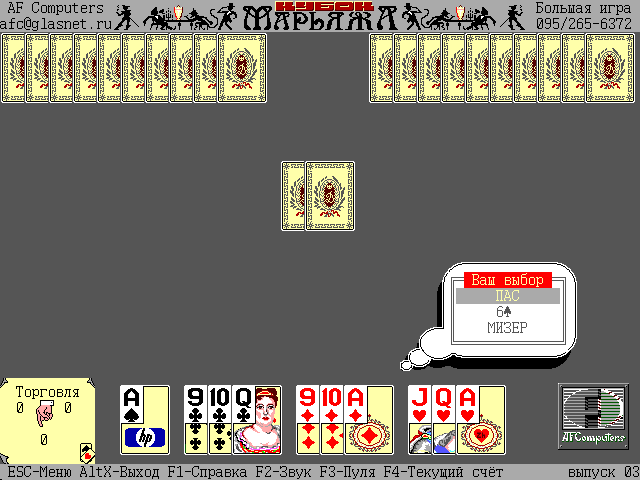
\includegraphics[scale=\FigScale]{examples/marriage/initial_not_patched.png}
\caption{"Торги"}
\end{figure}

Попробуем "подсмотреть" карты в "прикупе" в этой игре.

Для начала --- что мы знаем?
Игра под DOS, датируется 1997-м годом. IDA показывает имена стандартных функций вроде 
\TT{@GetImage\$q7Integert1t1t1m3Any} --- это "манглинг" типичный для Borland Pascal, что позволяет сделать вывод,
что сама игра написана на Паскале и скомпилирована Borland Pascal-ем.

Файлов около 10-и и некоторые имеют текстовую строку в заголовке "Marriage Image Library" --- вероятно,
это библиотеки спрайтов.

В IDA можно увидеть что используется функция \TT{@PutImage\$q7Integert1m3Any4Word}, которая, собственно,
рисует некий спрайт на экране.
Она вызывается по крайней мере из 8-и мест.
Чтобы узнать что происходит в каждом из этих 8-и мест, мы можем блокировать работу каждой функции и смотреть,
что будет происходить.
Например, первая ф-ция имеет адрес seg002:062E, и она заканчивается инструкцией \INS{retf 0Eh} на seg002:102A.
Это означает что метод вызовов ф-ций в Borland Pascal под DOS схож с stdcall --- вызываемая ф-ция должна сама
возвращать стек в состояние до того как началась передача аргументов.
В самом начале этой ф-ции вписываем инструкцию "retf 0eh", либо 3 байта: \TT{CA 0E 00}.
Запускаем "Марьяж" и внешне вроде бы ничего не изменилось.

Переходим ко второй ф-ции, которая активно использует \TT{@PutImage\$q7Integert1m3Any4Word}.
Она находится по адресу seg008:0AB5 и заканчивается инструкцией \INS{retf 0Ah}.
Вписываем эту инструкцию в самом начале и запускаем:

\begin{figure}[H]
\centering
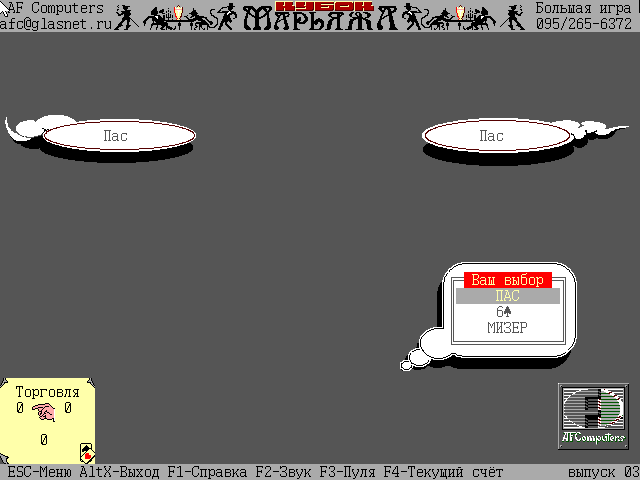
\includegraphics[scale=\FigScale]{examples/marriage/draw_card_bypass.png}
\caption{Карт нет}
\end{figure}

Карт не видно вообще. И видимо, эта функция их отображает, мы её заблокировали, и теперь карт не видно.
Назовем эту ф-цию в IDA \TT{draw\_card()}.
Помимо \TT{@PutImage\$q7Integert1m3Any4Word}, в этой ф-ции вызываются также ф-ции @SetColor\$q4Word, 
\TT{@SetFillStyle\$q4Wordt1}, \TT{@Bar\$q7Integert1t1t1}, \TT{@OutTextXY\$q7Integert16String}.

Сама ф-ция \TT{draw\_cards()} (её название мы дали ей сами только что) вызывается из 4-х мест.
Попробуем точно также "блокировать" каждую ф-цию.

Когда я "блокирую" вторую, по адресу seg008:0DF3 и запускаю программу, вижу такое:

\begin{figure}[H]
\centering
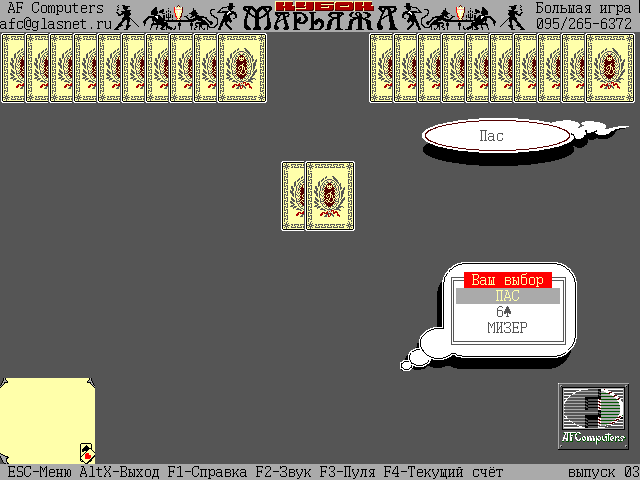
\includegraphics[scale=\FigScale]{examples/marriage/draw_players_cards.png}
\caption{Все карты кроме карт игрока}
\end{figure}

Видны все карты, кроме карт игрока. Видимо, эта функция рисует карты игрока. \\
Я переименовываю её в IDA в \TT{draw\_players\_cards()}.

Четвертая ф-ция, вызывающая \TT{draw\_cards()}, находится по адресу seg008:16B3, и когда я её "блокирую",
я вижу в игре такое:

\begin{figure}[H]
\centering
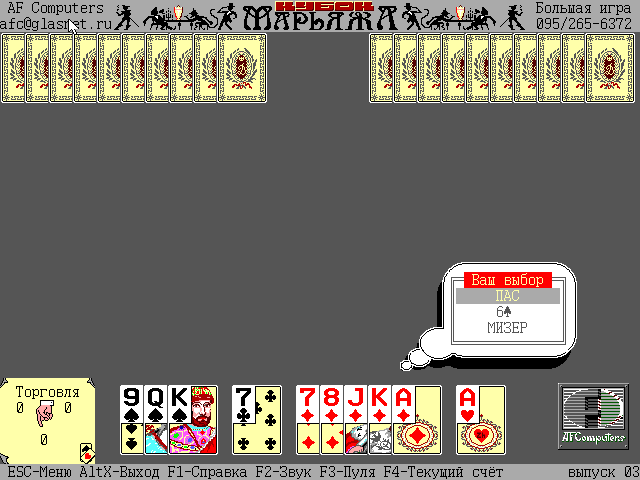
\includegraphics[scale=\FigScale]{examples/marriage/no_prikup.png}
\caption{"Прикупа" нет}
\end{figure}

Все карты есть, кроме "прикупа". Более того, эта ф-ция вызывает только \TT{draw\_cards()}, и только 2 раза.
Видимо эта ф-ция и отображает карты "прикупа".
Будем рассматривать её внимательнее.

\begin{lstlisting}
seg008:16B3 draw_prikup     proc far                ; CODE XREF: seg010:00B0
seg008:16B3                                         ; sub_15098+6
seg008:16B3
seg008:16B3 var_E           = word ptr -0Eh
seg008:16B3 var_C           = word ptr -0Ch
seg008:16B3 arg_0           = byte ptr  6
seg008:16B3
seg008:16B3                 enter   0Eh, 0
seg008:16B7                 mov     al, byte_2C0EA
seg008:16BA                 xor     ah, ah
seg008:16BC                 imul    ax, 23h
seg008:16BF                 mov     [bp+var_C], ax
seg008:16C2                 mov     al, byte_2C0EB
seg008:16C5                 xor     ah, ah
seg008:16C7                 imul    ax, 0Ah
seg008:16CA                 mov     [bp+var_E], ax
seg008:16CD                 cmp     [bp+arg_0], 0
seg008:16D1                 jnz     short loc_1334A
seg008:16D3                 cmp     byte_2BB08, 0
seg008:16D8                 jz      short loc_13356
seg008:16DA
seg008:16DA loc_1334A:                              ; CODE XREF: draw_prikup+1E
seg008:16DA                 mov     al, byte ptr word_32084
seg008:16DD                 mov     byte_293AD, al
seg008:16E0                 mov     al, byte ptr word_32086
seg008:16E3                 mov     byte_293AC, al
seg008:16E6
seg008:16E6 loc_13356:                              ; CODE XREF: draw_prikup+25
seg008:16E6                 mov     al, byte_293AC
seg008:16E9                 xor     ah, ah
seg008:16EB                 push    ax
seg008:16EC                 mov     al, byte_293AD
seg008:16EF                 xor     ah, ah
seg008:16F1                 push    ax
seg008:16F2                 push    [bp+var_C]
seg008:16F5                 push    [bp+var_E]
seg008:16F8                 cmp     [bp+arg_0], 0
seg008:16FC                 jnz     short loc_13379
seg008:16FE                 cmp     byte_2BB08, 0
seg008:1703                 jnz     short loc_13379
seg008:1705                 mov     al, 0
seg008:1707                 jmp     short loc_1337B
seg008:1709 ; ---------------------------------------------------------------------------
seg008:1709
seg008:1709 loc_13379:                              ; CODE XREF: draw_prikup+49
seg008:1709                                         ; draw_prikup+50
seg008:1709                 mov     al, 1
seg008:170B
seg008:170B loc_1337B:                              ; CODE XREF: draw_prikup+54
seg008:170B                 push    ax
seg008:170C                 push    cs
seg008:170D                 call    near ptr draw_card
seg008:1710                 mov     al, byte_2C0EA
seg008:1713                 xor     ah, ah
seg008:1715                 mov     si, ax
seg008:1717                 shl     ax, 1
seg008:1719                 add     ax, si
seg008:171B                 add     ax, [bp+var_C]
seg008:171E                 mov     [bp+var_C], ax
seg008:1721                 cmp     [bp+arg_0], 0
seg008:1725                 jnz     short loc_1339E
seg008:1727                 cmp     byte_2BB08, 0
seg008:172C                 jz      short loc_133AA
seg008:172E
seg008:172E loc_1339E:                              ; CODE XREF: draw_prikup+72
seg008:172E                 mov     al, byte ptr word_32088
seg008:1731                 mov     byte_293AD, al
seg008:1734                 mov     al, byte ptr word_3208A
seg008:1737                 mov     byte_293AC, al
seg008:173A
seg008:173A loc_133AA:                              ; CODE XREF: draw_prikup+79
seg008:173A                 mov     al, byte_293AC
seg008:173D                 xor     ah, ah
seg008:173F                 push    ax
seg008:1740                 mov     al, byte_293AD
seg008:1743                 xor     ah, ah
seg008:1745                 push    ax
seg008:1746                 push    [bp+var_C]
seg008:1749                 push    [bp+var_E]
seg008:174C                 cmp     [bp+arg_0], 0
seg008:1750                 jnz     short loc_133CD
seg008:1752                 cmp     byte_2BB08, 0
seg008:1757                 jnz     short loc_133CD
seg008:1759                 mov     al, 0
seg008:175B                 jmp     short loc_133CF
seg008:175D ; ---------------------------------------------------------------------------
seg008:175D
seg008:175D loc_133CD:                              ; CODE XREF: draw_prikup+9D
seg008:175D                                         ; draw_prikup+A4
seg008:175D                 mov     al, 1
seg008:175F
seg008:175F loc_133CF:                              ; CODE XREF: draw_prikup+A8
seg008:175F                 push    ax
seg008:1760                 push    cs
seg008:1761                 call    near ptr draw_card ; prikup #2
seg008:1764                 leave
seg008:1765                 retf    2
seg008:1765 draw_prikup     endp
\end{lstlisting}

Интересно посмотреть, как именно вызывается \TT{draw\_prikup()}. У нее только один аргумент.

Иногда она вызывается с аргументом 1:

\begin{lstlisting}
...
seg010:084C                 push    1
seg010:084E                 call    draw_prikup
...
\end{lstlisting}

А иногда с аргументом 0, причем вот в таком контексте, где уже есть другая знакомая функция:

\begin{lstlisting}
seg010:0067                 push    1
seg010:0069                 mov     al, byte_31F41
seg010:006C                 push    ax
seg010:006D                 call    sub_12FDC
seg010:0072                 push    1
seg010:0074                 mov     al, byte_31F41
seg010:0077                 push    ax
seg010:0078                 call    draw_players_cards
seg010:007D                 push    2
seg010:007F                 mov     al, byte_31F42
seg010:0082                 push    ax
seg010:0083                 call    sub_12FDC
seg010:0088                 push    2
seg010:008A                 mov     al, byte_31F42
seg010:008D                 push    ax
seg010:008E                 call    draw_players_cards
seg010:0093                 push    3
seg010:0095                 mov     al, byte_31F43
seg010:0098                 push    ax
seg010:0099                 call    sub_12FDC
seg010:009E                 push    3
seg010:00A0                 mov     al, byte_31F43
seg010:00A3                 push    ax
seg010:00A4                 call    draw_players_cards
seg010:00A9                 call    sub_1257A
seg010:00AE                 push    0
seg010:00B0                 call    draw_prikup
seg010:00B5                 mov     byte_2BB95, 0
\end{lstlisting}

Так что единственный аргумент у \TT{draw\_prikup()} может быть или 0 или 1, т.е., это, возможно, булевый тип.
На что он влияет внутри самой ф-ции?
При ближайшем рассмотрении видно, что входящий 0 или 1 передается в \TT{draw\_card()}, т.е., у последней тоже есть
булевый аргумент.
Помимо всего прочего, если передается 1, то по адресам seg008:16DA и seg008:172E копируются несколько байт
из одной группы глобальных переменных в другую.

Эксперимент: здесь 4 раза сравнивается единственный аргумент с 0 и далее следует \INS{JNZ}.
Что если сравнение будет происходит с 1, и, таким образом, работа функции \TT{draw\_prikup()} будет обратной?
Патчим и запускаем:

\begin{figure}[H]
\centering
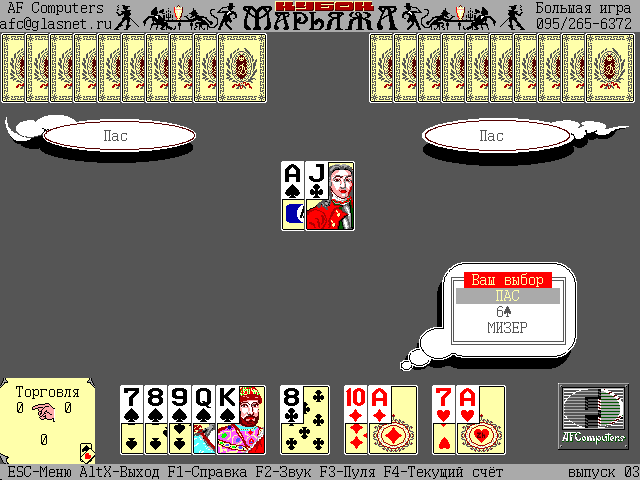
\includegraphics[scale=\FigScale]{examples/marriage/patch1.png}
\caption{"Прикуп" открыт}
\end{figure}

"Прикуп" открыт, но когда я делаю "заказ", и, по логике вещей, "прикуп" теперь должен стать открытым,
он наоборот становится закрытым:

\begin{figure}[H]
\centering
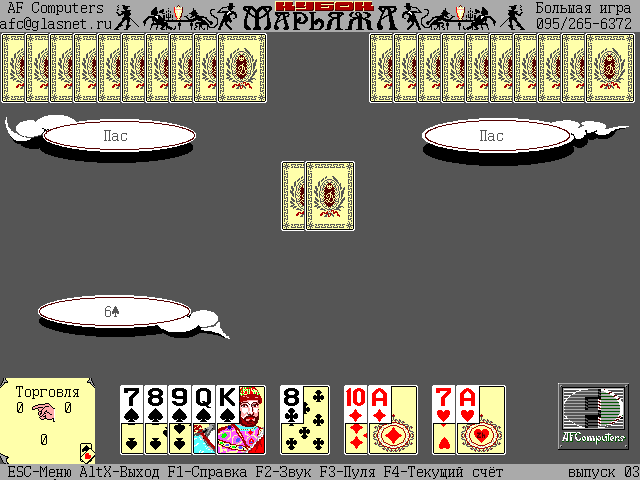
\includegraphics[scale=\FigScale]{examples/marriage/patch2.png}
\caption{"Прикуп" закрыт}
\end{figure}

Всё ясно: если аргумент \TT{draw\_prikup()} нулевой, то карты рисуются рубашкой вверх, если 1, то открытые.
Этот же аргумент передается в \TT{draw\_card()} --- эта ф-ция может рисовать и открытые и закрытые карты.

Пропатчить "Марьяж" теперь легко, достаточно исправить все условные переходы так, как будто бы в ф-цию
всегда приходит 1 в аргументе и тогда "прикуп" всегда будет открыт.

Но что за байты копируются в seg008:16DA и seg008:172E?
Я попробовал забить инструкции копирования \MOV \NOP{}-ами --- "прикуп" вообще перестал отображаться.

Тогда я сделал так, чтобы всегда записывалась 1:

\begin{lstlisting}
...
00004B5A: B001                           mov         al,1
00004B5C: 90                             nop
00004B5D: A26D08                         mov         [0086D],al
00004B60: B001                           mov         al,1
00004B62: 90                             nop
00004B63: A26C08                         mov         [0086C],al
...
\end{lstlisting}

Тогда "прикуп" отображается как два пиковых туза.
А если первый байт --- 2, а второй --- 1, получается трефовый туз.
Видимо так и кодируется масть карты, а затем и сама карта.
% TODO \ref{} сюда о том, как можно передавать аргументы в глоб.переменных
А \TT{draw\_card()} затем считывает эту информацию из пары глобальных переменных.
А копируется она тоже из глобальных переменных, где собственно и находится состояние карт у игроков и в прикупе
после случайной тасовки.
Но нельзя забывать что если мы сделаем так, что в "прикупе" всегда будет 2 пиковых туза, это будет только
на экране так отображаться, а в памяти состояние карт останется таким же, как и после тасовки.

Я также пробовал сделать пранк: во время торгов одна карта "прикупа" открыта, а вторая закрыта, а после "заказа",
наоборот, первая закрыта, а вторая открывается. В качестве упражнения, вы можете попробовать сделать так.

Еще кое-что: чтобы сделать прикуп открытым, ведь можно же найти место где вызывается \TT{draw\_prikup()} и поменять 0
на 1. Можно, только это место не в головой marriage.exe, а в marriage.000, а это DOS-овский оверлей (начинается
с сигнатуры "FBOV").

В качестве упражнения, можно попробовать подсматривать состояние всех карт, и у обоих игроков.
Для этого нужно отладчиком смотреть состояние глобальной памяти рядом с тем, откуда считываются обе карты
прикупа.

Файлы: \\
оригинальная версия: \url{http://beginners.re/examples/marriage/original.zip}, \\
пропатченная мною версия: \url{http://beginners.re/examples/marriage/patched.zip} 
(все 4 условных перехода после \TT{cmp [bp+arg\_0], 0} заменены на \JMP).

}

\renewcommand{\CURPATH}{advanced/115_loop_iterators}
\chapter{\RU{Конверсия строки в число}\EN{String to number conversion} (atoi())}

\myindex{\CStandardLibrary!atoi()}
\RU{Попробуем реализовать стандарту функцию Си atoi().}
\EN{Let's try to reimplement the standard atoi() C function.}

\section{\RU{Простой пример}\EN{Simple example}}

\RU{Это самый простой способ прочитать число, представленное в кодировке \ac{ASCII}.}
\EN{Here is the simplest possible way to read a number represented in \ac{ASCII} encoding.}
\RU{Он не защищен от ошибок: символ отличный от цифры приведет к неверному результату.}
\EN{It's not error-prone: a character other than a digit leads to incorrect result.}

\lstinputlisting{\CURPATH/atoi.c}

\RU{То, что делает алгоритм это просто считывает цифры слева направо.}
\EN{So what the algorithm does is just reading digits from left to right.}
\RU{Символ нуля в \ac{ASCII} вычитается из каждой цифры.}
\EN{The zero \ac{ASCII} character is subtracted from each digit. }
\RU{Цифры от \q{0} до \q{9} расположены по порядку в таблице \ac{ASCII}, так что мы даже можем
и не знать точного значения символа \q{0}.}
\EN{The digits from \q{0} to \q{9} are consecutive in the \ac{ASCII} table, so 
we do not even need to know the exact value of the \q{0} character.}
\RU{Всё что нам нужно знать это то что \q{0} минус \q{0}\EMDASH{}это 0, а \q{9} минус \q{0} это 9, \etc{}.}
\EN{All we need to know is that \q{0} minus \q{0} is 0, \q{9} minus \q{0}'is 9 and so on.}
\RU{Вычитание \q{0} от каждого символа в итоге дает число от 0 до 9 включительно.}
\EN{Subtracting \q{0} from each character results in a number from 0 to 9 inclusive.}
\RU{Любой другой символ, конечно, приведет к неверному результату!}
\EN{Any other character leads to an incorrect result, of course!}
\RU{Каждая цифра добавляется к итоговому результату (в переменной \q{rt}), но итоговый результат
также умножается на 10 на каждой цифре.}
\EN{Each digit has to be added to the final result (in variable \q{rt}), but the final result
is also multiplied by 10 at each digit.}
\RU{Другими словами, на каждой итерации, результат сдвигается влево на одну позицию в десятичном виде.}
\EN{In other words, the result is shifted left by one position in decimal form on each iteration.}
\RU{Самая последняя цифра прибавляется, но не сдвигается.}
\EN{The last digit is added, but there is no no shift.}

\subsection{\Optimizing MSVC 2013 x64}

\lstinputlisting[caption=\Optimizing MSVC 2013 x64]{\CURPATH/atoi.asm.MSVC2013.x64.Ox.\LANG}

\RU{Символы загружаются в двух местах: первый символ и все последующие символы.}
\EN{A character can be loaded in two places: the first character and all subsequent characters.}
\RU{Это сделано для перегруппировки цикла.}\EN{This is done for loop regrouping.}
\myindex{x86!\Instructions!LEA}
\RU{Здесь нет инструкции для умножения на 10, вместо этого две LEA делают это же.}
\EN{There is no instruction for multiplication by 10, two LEA instruction do this instead.}
\myindex{x86!\Instructions!ADD}
\myindex{x86!\Instructions!SUB}
\RU{MSVC иногда использует инструкцию ADD с отрицательной константой вместо SUB.}
\EN{MSVC sometimes uses the ADD instruction with a negative constant instead of SUB.}
\RU{Это тот случай}\EN{This is the case}.
\RU{Честно говоря, трудно сказать, чем это лучше, чем SUB.}
\EN{It's very hard to say why this is better then SUB.}
\RU{Но MSVC делает так часто}\EN{But MSVC does this often}.

\subsection{\Optimizing GCC 4.9.1 x64}

\Optimizing GCC 4.9.1 \RU{более краток, но здесь есть одна лишняя инструкция RET в конце.}
\EN{is more concise, but there is one redundant RET instruction at the end.}
\RU{Одной было бы достаточно}\EN{One would be enough}.

\lstinputlisting[caption=\Optimizing GCC 4.9.1 x64]{\CURPATH/atoi.s.GCC491.O3.x64.\LANG}

\subsection{\OptimizingKeilVI (\ARMMode)}

\lstinputlisting[caption=\OptimizingKeilVI (\ARMMode)]{\CURPATH/atoi.s.ARM.O3.\LANG}

\subsection{\OptimizingKeilVI (\ThumbMode)}

\lstinputlisting[caption=\OptimizingKeilVI (\ThumbMode)]{\CURPATH/atoi.s.thumb.O3.\LANG}

\RU{Интересно, из школьного курса математики мы можем помнить что порядок операций сложения и вычитания
не играет роли.}
\EN{Interestingly, from school mathematics we may remember that the order of addition and 
subtraction operations doesn't matter.}
\RU{Это наш случай: в начале вычисляется выражение $rt*10 - '0'$, затем к нему прибавляется 
значение входного символа.}
\EN{That's our case: first, the $rt*10 - '0'$ expression is computed, then the input character value 
is added to it.}
\RU{Действительно, результат тот же, но компилятор немного всё перегруппировал.}
\EN{Indeed, the result is the same, but the compiler did some regrouping.}

\subsection{\Optimizing GCC 4.9.1 ARM64}

\RU{Компилятор для ARM64 может использовать суффикс инструкции, задающий пре-инкремент:}
\EN{The ARM64 compiler can use the pre-increment instruction suffix:}

\lstinputlisting[caption=\Optimizing GCC 4.9.1 ARM64]{\CURPATH/atoi.s.GCC49.ARM64.O3.\LANG}

\section{\RU{Немного расширенный пример}\EN{A slightly advanced example}}

\RU{Новый пример более расширенный, теперь здесь есть проверка знака \q{минус} в самом начале,
и еще он может сообщать об ошибке если не-цифра была найдена во входной строке:}
\EN{My new code snippet is more advanced, now it checks for the \q{minus} sign at the first character
and reports an error if a non-digit was found in the input string:}

\lstinputlisting{\CURPATH/atoi2.c}

\subsection{\Optimizing GCC 4.9.1 x64}

\lstinputlisting[caption=\Optimizing GCC 4.9.1 x64]{\CURPATH/atoi2.s.GCC491.O3.x64.\LANG}

\myindex{x86!\Instructions!NEG}
\RU{Если знак \q{минус} был найден в начале строки, инструкция NEG будет исполнена в конце.}
\EN{If the \q{minus} sign was encountered at the string start, the NEG instruction is to be executed at the end.}
\RU{Она просто меняет знак числа}\EN{It just negates the number}.

\label{one_comparison_instead_of_two}
\RU{Еще кое-что надо отметить}\EN{There is one more thing that needs mentioning}.
\RU{Как среднестатистический программист будет проверять, является ли символ цифрой?}
\EN{How would a common programmer check if the character is not a digit?}
\RU{Так же, как и у нас в исходном коде}\EN{Just how we have it in the source code}:

\begin{lstlisting}
if (*s<'0' || *s>'9')
    ...
\end{lstlisting}

\RU{Здесь две операции сравнения}\EN{There are two comparison operations}.
\RU{Но что интересно, так это то что мы можем заменить обе операции на одну:}
\EN{What is interesting is that we can replace both operations by single one:}
\RU{просто вычитайте \q{0} из значения символа}\EN{just subtract \q{0} from character value},
\RU{считается результат за беззнаковое значение (это важно) и проверьте, не больше ли он чем 9.}
\EN{treat result as unsigned value (this is important) and check if it's greater than 9.}

\RU{Например, скажем, строка на входе имеет символ точки (\q{.}), которая имеет код 46 в таблице \ac{ASCII}.}
\EN{For example, let's say that the user input contains the dot character (\q{.}) which has \ac{ASCII} code 46.}
$46-48=-2$ \RU{если считать результат за знаковое число}\EN{if we treat the result as a signed number}.
\RU{Действительно, символ точки расположен на два места раньше, чем символ \q{0} в таблице \ac{ASCII}.}
\EN{Indeed, the dot character is located two places earlier than the \q{0} character in the \ac{ASCII} table.}
\RU{Но это}\EN{But it is} \TT{0xFFFFFFFE} (4294967294) \RU{если считать результат за беззнаковое значение, 
и это точно больше чем 9!}
\EN{if we treat the result as an unsigned value, and that's definitely bigger than 9!}

\RU{Компиляторы часто так делают, важно распознавать эти трюки.}
\EN{The compilers do this often, so it's important to recognize these tricks.}

\EN{Another example of it in this book}\RU{Еще один пример подобного в этой книге}: 
\myref{toupper_one_comparison}.

\Optimizing MSVC 2013 x64 \RU{применяет те же трюки}\EN{does the same tricks}.

\subsection{\OptimizingKeilVI (\ARMMode)}

\lstinputlisting[caption=\OptimizingKeilVI (\ARMMode),numbers=left]{\CURPATH/atoi2.s.ARM.O3.\LANG}

\RU{В 32-битном ARM нет инструкции NEG, так что вместо этого используется операция \q{Reverse Subtraction}
(строка 31).}
\EN{There is no NEG instruction in 32-bit ARM, so the \q{Reverse Subtraction} operation (line 31) 
is used here.}
\RU{Она сработает если результат инструкции CMP (на строке 29) был \q{Not Equal} 
(не равно, отсюда суффикс -NE suffix).}
\EN{It is triggered if the result of the CMP instruction (at line 29) was \q{Not Equal} (hence -NE suffix).}
\myindex{ARM!\Instructions!RSB}
\RU{Что делает RSBNE это просто вычитает результирующее значение из нуля.}
\EN{So what RSBNE does is to subtract the resulting value from 0.}
\RU{Она работает, как и обычное вычитание, но меняет местами операнды.}
\EN{It works just like the regular subtraction operation, but swaps operands.}
\RU{Вычитание любого числа из нуля это смена знака}
\EN{Subtracting any number from 0 results in negation}: $0-x=-x$.

\RU{Код для режима Thumb почти такой же.}
\EN{Thumb mode code is mostly the same.}

\myindex{ARM!\Instructions!NEG}
GCC 4.9 \ForENRU ARM64 \RU{может использовать инструкцию NEG, доступную в}
\EN{can use the NEG instruction, which is available in} ARM64.

\section{\Exercise{}}

\myindex{Fuzzing}
\EN{Oh, by the way, security researchers deals often with unpredictable behaviour of program while handling of incorrect data.}
\RU{Кстати, security research-еры часто имеют дело с непредсказуемым поведением программ во время обработки некорректных данных.}
\RU{Например, во время fuzzing-а.}
\EN{For example, while fuzzing.}
\EN{As an exercise, you may try to enter non-digit characters and see what happens.}
\RU{В качестве упражнения, вы можете попробовать ввести символы не относящиеся к числам и посмотреть, что случится.}
\EN{Try to explain, what happened and why.}
\RU{Попробуйте объяснить, что произошло, и почему.}




\renewcommand{\CURPATH}{advanced/117_duff_device}
\chapter{\RU{Конверсия строки в число}\EN{String to number conversion} (atoi())}

\myindex{\CStandardLibrary!atoi()}
\RU{Попробуем реализовать стандарту функцию Си atoi().}
\EN{Let's try to reimplement the standard atoi() C function.}

\section{\RU{Простой пример}\EN{Simple example}}

\RU{Это самый простой способ прочитать число, представленное в кодировке \ac{ASCII}.}
\EN{Here is the simplest possible way to read a number represented in \ac{ASCII} encoding.}
\RU{Он не защищен от ошибок: символ отличный от цифры приведет к неверному результату.}
\EN{It's not error-prone: a character other than a digit leads to incorrect result.}

\lstinputlisting{\CURPATH/atoi.c}

\RU{То, что делает алгоритм это просто считывает цифры слева направо.}
\EN{So what the algorithm does is just reading digits from left to right.}
\RU{Символ нуля в \ac{ASCII} вычитается из каждой цифры.}
\EN{The zero \ac{ASCII} character is subtracted from each digit. }
\RU{Цифры от \q{0} до \q{9} расположены по порядку в таблице \ac{ASCII}, так что мы даже можем
и не знать точного значения символа \q{0}.}
\EN{The digits from \q{0} to \q{9} are consecutive in the \ac{ASCII} table, so 
we do not even need to know the exact value of the \q{0} character.}
\RU{Всё что нам нужно знать это то что \q{0} минус \q{0}\EMDASH{}это 0, а \q{9} минус \q{0} это 9, \etc{}.}
\EN{All we need to know is that \q{0} minus \q{0} is 0, \q{9} minus \q{0}'is 9 and so on.}
\RU{Вычитание \q{0} от каждого символа в итоге дает число от 0 до 9 включительно.}
\EN{Subtracting \q{0} from each character results in a number from 0 to 9 inclusive.}
\RU{Любой другой символ, конечно, приведет к неверному результату!}
\EN{Any other character leads to an incorrect result, of course!}
\RU{Каждая цифра добавляется к итоговому результату (в переменной \q{rt}), но итоговый результат
также умножается на 10 на каждой цифре.}
\EN{Each digit has to be added to the final result (in variable \q{rt}), but the final result
is also multiplied by 10 at each digit.}
\RU{Другими словами, на каждой итерации, результат сдвигается влево на одну позицию в десятичном виде.}
\EN{In other words, the result is shifted left by one position in decimal form on each iteration.}
\RU{Самая последняя цифра прибавляется, но не сдвигается.}
\EN{The last digit is added, but there is no no shift.}

\subsection{\Optimizing MSVC 2013 x64}

\lstinputlisting[caption=\Optimizing MSVC 2013 x64]{\CURPATH/atoi.asm.MSVC2013.x64.Ox.\LANG}

\RU{Символы загружаются в двух местах: первый символ и все последующие символы.}
\EN{A character can be loaded in two places: the first character and all subsequent characters.}
\RU{Это сделано для перегруппировки цикла.}\EN{This is done for loop regrouping.}
\myindex{x86!\Instructions!LEA}
\RU{Здесь нет инструкции для умножения на 10, вместо этого две LEA делают это же.}
\EN{There is no instruction for multiplication by 10, two LEA instruction do this instead.}
\myindex{x86!\Instructions!ADD}
\myindex{x86!\Instructions!SUB}
\RU{MSVC иногда использует инструкцию ADD с отрицательной константой вместо SUB.}
\EN{MSVC sometimes uses the ADD instruction with a negative constant instead of SUB.}
\RU{Это тот случай}\EN{This is the case}.
\RU{Честно говоря, трудно сказать, чем это лучше, чем SUB.}
\EN{It's very hard to say why this is better then SUB.}
\RU{Но MSVC делает так часто}\EN{But MSVC does this often}.

\subsection{\Optimizing GCC 4.9.1 x64}

\Optimizing GCC 4.9.1 \RU{более краток, но здесь есть одна лишняя инструкция RET в конце.}
\EN{is more concise, but there is one redundant RET instruction at the end.}
\RU{Одной было бы достаточно}\EN{One would be enough}.

\lstinputlisting[caption=\Optimizing GCC 4.9.1 x64]{\CURPATH/atoi.s.GCC491.O3.x64.\LANG}

\subsection{\OptimizingKeilVI (\ARMMode)}

\lstinputlisting[caption=\OptimizingKeilVI (\ARMMode)]{\CURPATH/atoi.s.ARM.O3.\LANG}

\subsection{\OptimizingKeilVI (\ThumbMode)}

\lstinputlisting[caption=\OptimizingKeilVI (\ThumbMode)]{\CURPATH/atoi.s.thumb.O3.\LANG}

\RU{Интересно, из школьного курса математики мы можем помнить что порядок операций сложения и вычитания
не играет роли.}
\EN{Interestingly, from school mathematics we may remember that the order of addition and 
subtraction operations doesn't matter.}
\RU{Это наш случай: в начале вычисляется выражение $rt*10 - '0'$, затем к нему прибавляется 
значение входного символа.}
\EN{That's our case: first, the $rt*10 - '0'$ expression is computed, then the input character value 
is added to it.}
\RU{Действительно, результат тот же, но компилятор немного всё перегруппировал.}
\EN{Indeed, the result is the same, but the compiler did some regrouping.}

\subsection{\Optimizing GCC 4.9.1 ARM64}

\RU{Компилятор для ARM64 может использовать суффикс инструкции, задающий пре-инкремент:}
\EN{The ARM64 compiler can use the pre-increment instruction suffix:}

\lstinputlisting[caption=\Optimizing GCC 4.9.1 ARM64]{\CURPATH/atoi.s.GCC49.ARM64.O3.\LANG}

\section{\RU{Немного расширенный пример}\EN{A slightly advanced example}}

\RU{Новый пример более расширенный, теперь здесь есть проверка знака \q{минус} в самом начале,
и еще он может сообщать об ошибке если не-цифра была найдена во входной строке:}
\EN{My new code snippet is more advanced, now it checks for the \q{minus} sign at the first character
and reports an error if a non-digit was found in the input string:}

\lstinputlisting{\CURPATH/atoi2.c}

\subsection{\Optimizing GCC 4.9.1 x64}

\lstinputlisting[caption=\Optimizing GCC 4.9.1 x64]{\CURPATH/atoi2.s.GCC491.O3.x64.\LANG}

\myindex{x86!\Instructions!NEG}
\RU{Если знак \q{минус} был найден в начале строки, инструкция NEG будет исполнена в конце.}
\EN{If the \q{minus} sign was encountered at the string start, the NEG instruction is to be executed at the end.}
\RU{Она просто меняет знак числа}\EN{It just negates the number}.

\label{one_comparison_instead_of_two}
\RU{Еще кое-что надо отметить}\EN{There is one more thing that needs mentioning}.
\RU{Как среднестатистический программист будет проверять, является ли символ цифрой?}
\EN{How would a common programmer check if the character is not a digit?}
\RU{Так же, как и у нас в исходном коде}\EN{Just how we have it in the source code}:

\begin{lstlisting}
if (*s<'0' || *s>'9')
    ...
\end{lstlisting}

\RU{Здесь две операции сравнения}\EN{There are two comparison operations}.
\RU{Но что интересно, так это то что мы можем заменить обе операции на одну:}
\EN{What is interesting is that we can replace both operations by single one:}
\RU{просто вычитайте \q{0} из значения символа}\EN{just subtract \q{0} from character value},
\RU{считается результат за беззнаковое значение (это важно) и проверьте, не больше ли он чем 9.}
\EN{treat result as unsigned value (this is important) and check if it's greater than 9.}

\RU{Например, скажем, строка на входе имеет символ точки (\q{.}), которая имеет код 46 в таблице \ac{ASCII}.}
\EN{For example, let's say that the user input contains the dot character (\q{.}) which has \ac{ASCII} code 46.}
$46-48=-2$ \RU{если считать результат за знаковое число}\EN{if we treat the result as a signed number}.
\RU{Действительно, символ точки расположен на два места раньше, чем символ \q{0} в таблице \ac{ASCII}.}
\EN{Indeed, the dot character is located two places earlier than the \q{0} character in the \ac{ASCII} table.}
\RU{Но это}\EN{But it is} \TT{0xFFFFFFFE} (4294967294) \RU{если считать результат за беззнаковое значение, 
и это точно больше чем 9!}
\EN{if we treat the result as an unsigned value, and that's definitely bigger than 9!}

\RU{Компиляторы часто так делают, важно распознавать эти трюки.}
\EN{The compilers do this often, so it's important to recognize these tricks.}

\EN{Another example of it in this book}\RU{Еще один пример подобного в этой книге}: 
\myref{toupper_one_comparison}.

\Optimizing MSVC 2013 x64 \RU{применяет те же трюки}\EN{does the same tricks}.

\subsection{\OptimizingKeilVI (\ARMMode)}

\lstinputlisting[caption=\OptimizingKeilVI (\ARMMode),numbers=left]{\CURPATH/atoi2.s.ARM.O3.\LANG}

\RU{В 32-битном ARM нет инструкции NEG, так что вместо этого используется операция \q{Reverse Subtraction}
(строка 31).}
\EN{There is no NEG instruction in 32-bit ARM, so the \q{Reverse Subtraction} operation (line 31) 
is used here.}
\RU{Она сработает если результат инструкции CMP (на строке 29) был \q{Not Equal} 
(не равно, отсюда суффикс -NE suffix).}
\EN{It is triggered if the result of the CMP instruction (at line 29) was \q{Not Equal} (hence -NE suffix).}
\myindex{ARM!\Instructions!RSB}
\RU{Что делает RSBNE это просто вычитает результирующее значение из нуля.}
\EN{So what RSBNE does is to subtract the resulting value from 0.}
\RU{Она работает, как и обычное вычитание, но меняет местами операнды.}
\EN{It works just like the regular subtraction operation, but swaps operands.}
\RU{Вычитание любого числа из нуля это смена знака}
\EN{Subtracting any number from 0 results in negation}: $0-x=-x$.

\RU{Код для режима Thumb почти такой же.}
\EN{Thumb mode code is mostly the same.}

\myindex{ARM!\Instructions!NEG}
GCC 4.9 \ForENRU ARM64 \RU{может использовать инструкцию NEG, доступную в}
\EN{can use the NEG instruction, which is available in} ARM64.

\section{\Exercise{}}

\myindex{Fuzzing}
\EN{Oh, by the way, security researchers deals often with unpredictable behaviour of program while handling of incorrect data.}
\RU{Кстати, security research-еры часто имеют дело с непредсказуемым поведением программ во время обработки некорректных данных.}
\RU{Например, во время fuzzing-а.}
\EN{For example, while fuzzing.}
\EN{As an exercise, you may try to enter non-digit characters and see what happens.}
\RU{В качестве упражнения, вы можете попробовать ввести символы не относящиеся к числам и посмотреть, что случится.}
\EN{Try to explain, what happened and why.}
\RU{Попробуйте объяснить, что произошло, и почему.}




\renewcommand{\CURPATH}{advanced/120_division_by_9}
\chapter{\RU{Конверсия строки в число}\EN{String to number conversion} (atoi())}

\myindex{\CStandardLibrary!atoi()}
\RU{Попробуем реализовать стандарту функцию Си atoi().}
\EN{Let's try to reimplement the standard atoi() C function.}

\section{\RU{Простой пример}\EN{Simple example}}

\RU{Это самый простой способ прочитать число, представленное в кодировке \ac{ASCII}.}
\EN{Here is the simplest possible way to read a number represented in \ac{ASCII} encoding.}
\RU{Он не защищен от ошибок: символ отличный от цифры приведет к неверному результату.}
\EN{It's not error-prone: a character other than a digit leads to incorrect result.}

\lstinputlisting{\CURPATH/atoi.c}

\RU{То, что делает алгоритм это просто считывает цифры слева направо.}
\EN{So what the algorithm does is just reading digits from left to right.}
\RU{Символ нуля в \ac{ASCII} вычитается из каждой цифры.}
\EN{The zero \ac{ASCII} character is subtracted from each digit. }
\RU{Цифры от \q{0} до \q{9} расположены по порядку в таблице \ac{ASCII}, так что мы даже можем
и не знать точного значения символа \q{0}.}
\EN{The digits from \q{0} to \q{9} are consecutive in the \ac{ASCII} table, so 
we do not even need to know the exact value of the \q{0} character.}
\RU{Всё что нам нужно знать это то что \q{0} минус \q{0}\EMDASH{}это 0, а \q{9} минус \q{0} это 9, \etc{}.}
\EN{All we need to know is that \q{0} minus \q{0} is 0, \q{9} minus \q{0}'is 9 and so on.}
\RU{Вычитание \q{0} от каждого символа в итоге дает число от 0 до 9 включительно.}
\EN{Subtracting \q{0} from each character results in a number from 0 to 9 inclusive.}
\RU{Любой другой символ, конечно, приведет к неверному результату!}
\EN{Any other character leads to an incorrect result, of course!}
\RU{Каждая цифра добавляется к итоговому результату (в переменной \q{rt}), но итоговый результат
также умножается на 10 на каждой цифре.}
\EN{Each digit has to be added to the final result (in variable \q{rt}), but the final result
is also multiplied by 10 at each digit.}
\RU{Другими словами, на каждой итерации, результат сдвигается влево на одну позицию в десятичном виде.}
\EN{In other words, the result is shifted left by one position in decimal form on each iteration.}
\RU{Самая последняя цифра прибавляется, но не сдвигается.}
\EN{The last digit is added, but there is no no shift.}

\subsection{\Optimizing MSVC 2013 x64}

\lstinputlisting[caption=\Optimizing MSVC 2013 x64]{\CURPATH/atoi.asm.MSVC2013.x64.Ox.\LANG}

\RU{Символы загружаются в двух местах: первый символ и все последующие символы.}
\EN{A character can be loaded in two places: the first character and all subsequent characters.}
\RU{Это сделано для перегруппировки цикла.}\EN{This is done for loop regrouping.}
\myindex{x86!\Instructions!LEA}
\RU{Здесь нет инструкции для умножения на 10, вместо этого две LEA делают это же.}
\EN{There is no instruction for multiplication by 10, two LEA instruction do this instead.}
\myindex{x86!\Instructions!ADD}
\myindex{x86!\Instructions!SUB}
\RU{MSVC иногда использует инструкцию ADD с отрицательной константой вместо SUB.}
\EN{MSVC sometimes uses the ADD instruction with a negative constant instead of SUB.}
\RU{Это тот случай}\EN{This is the case}.
\RU{Честно говоря, трудно сказать, чем это лучше, чем SUB.}
\EN{It's very hard to say why this is better then SUB.}
\RU{Но MSVC делает так часто}\EN{But MSVC does this often}.

\subsection{\Optimizing GCC 4.9.1 x64}

\Optimizing GCC 4.9.1 \RU{более краток, но здесь есть одна лишняя инструкция RET в конце.}
\EN{is more concise, but there is one redundant RET instruction at the end.}
\RU{Одной было бы достаточно}\EN{One would be enough}.

\lstinputlisting[caption=\Optimizing GCC 4.9.1 x64]{\CURPATH/atoi.s.GCC491.O3.x64.\LANG}

\subsection{\OptimizingKeilVI (\ARMMode)}

\lstinputlisting[caption=\OptimizingKeilVI (\ARMMode)]{\CURPATH/atoi.s.ARM.O3.\LANG}

\subsection{\OptimizingKeilVI (\ThumbMode)}

\lstinputlisting[caption=\OptimizingKeilVI (\ThumbMode)]{\CURPATH/atoi.s.thumb.O3.\LANG}

\RU{Интересно, из школьного курса математики мы можем помнить что порядок операций сложения и вычитания
не играет роли.}
\EN{Interestingly, from school mathematics we may remember that the order of addition and 
subtraction operations doesn't matter.}
\RU{Это наш случай: в начале вычисляется выражение $rt*10 - '0'$, затем к нему прибавляется 
значение входного символа.}
\EN{That's our case: first, the $rt*10 - '0'$ expression is computed, then the input character value 
is added to it.}
\RU{Действительно, результат тот же, но компилятор немного всё перегруппировал.}
\EN{Indeed, the result is the same, but the compiler did some regrouping.}

\subsection{\Optimizing GCC 4.9.1 ARM64}

\RU{Компилятор для ARM64 может использовать суффикс инструкции, задающий пре-инкремент:}
\EN{The ARM64 compiler can use the pre-increment instruction suffix:}

\lstinputlisting[caption=\Optimizing GCC 4.9.1 ARM64]{\CURPATH/atoi.s.GCC49.ARM64.O3.\LANG}

\section{\RU{Немного расширенный пример}\EN{A slightly advanced example}}

\RU{Новый пример более расширенный, теперь здесь есть проверка знака \q{минус} в самом начале,
и еще он может сообщать об ошибке если не-цифра была найдена во входной строке:}
\EN{My new code snippet is more advanced, now it checks for the \q{minus} sign at the first character
and reports an error if a non-digit was found in the input string:}

\lstinputlisting{\CURPATH/atoi2.c}

\subsection{\Optimizing GCC 4.9.1 x64}

\lstinputlisting[caption=\Optimizing GCC 4.9.1 x64]{\CURPATH/atoi2.s.GCC491.O3.x64.\LANG}

\myindex{x86!\Instructions!NEG}
\RU{Если знак \q{минус} был найден в начале строки, инструкция NEG будет исполнена в конце.}
\EN{If the \q{minus} sign was encountered at the string start, the NEG instruction is to be executed at the end.}
\RU{Она просто меняет знак числа}\EN{It just negates the number}.

\label{one_comparison_instead_of_two}
\RU{Еще кое-что надо отметить}\EN{There is one more thing that needs mentioning}.
\RU{Как среднестатистический программист будет проверять, является ли символ цифрой?}
\EN{How would a common programmer check if the character is not a digit?}
\RU{Так же, как и у нас в исходном коде}\EN{Just how we have it in the source code}:

\begin{lstlisting}
if (*s<'0' || *s>'9')
    ...
\end{lstlisting}

\RU{Здесь две операции сравнения}\EN{There are two comparison operations}.
\RU{Но что интересно, так это то что мы можем заменить обе операции на одну:}
\EN{What is interesting is that we can replace both operations by single one:}
\RU{просто вычитайте \q{0} из значения символа}\EN{just subtract \q{0} from character value},
\RU{считается результат за беззнаковое значение (это важно) и проверьте, не больше ли он чем 9.}
\EN{treat result as unsigned value (this is important) and check if it's greater than 9.}

\RU{Например, скажем, строка на входе имеет символ точки (\q{.}), которая имеет код 46 в таблице \ac{ASCII}.}
\EN{For example, let's say that the user input contains the dot character (\q{.}) which has \ac{ASCII} code 46.}
$46-48=-2$ \RU{если считать результат за знаковое число}\EN{if we treat the result as a signed number}.
\RU{Действительно, символ точки расположен на два места раньше, чем символ \q{0} в таблице \ac{ASCII}.}
\EN{Indeed, the dot character is located two places earlier than the \q{0} character in the \ac{ASCII} table.}
\RU{Но это}\EN{But it is} \TT{0xFFFFFFFE} (4294967294) \RU{если считать результат за беззнаковое значение, 
и это точно больше чем 9!}
\EN{if we treat the result as an unsigned value, and that's definitely bigger than 9!}

\RU{Компиляторы часто так делают, важно распознавать эти трюки.}
\EN{The compilers do this often, so it's important to recognize these tricks.}

\EN{Another example of it in this book}\RU{Еще один пример подобного в этой книге}: 
\myref{toupper_one_comparison}.

\Optimizing MSVC 2013 x64 \RU{применяет те же трюки}\EN{does the same tricks}.

\subsection{\OptimizingKeilVI (\ARMMode)}

\lstinputlisting[caption=\OptimizingKeilVI (\ARMMode),numbers=left]{\CURPATH/atoi2.s.ARM.O3.\LANG}

\RU{В 32-битном ARM нет инструкции NEG, так что вместо этого используется операция \q{Reverse Subtraction}
(строка 31).}
\EN{There is no NEG instruction in 32-bit ARM, so the \q{Reverse Subtraction} operation (line 31) 
is used here.}
\RU{Она сработает если результат инструкции CMP (на строке 29) был \q{Not Equal} 
(не равно, отсюда суффикс -NE suffix).}
\EN{It is triggered if the result of the CMP instruction (at line 29) was \q{Not Equal} (hence -NE suffix).}
\myindex{ARM!\Instructions!RSB}
\RU{Что делает RSBNE это просто вычитает результирующее значение из нуля.}
\EN{So what RSBNE does is to subtract the resulting value from 0.}
\RU{Она работает, как и обычное вычитание, но меняет местами операнды.}
\EN{It works just like the regular subtraction operation, but swaps operands.}
\RU{Вычитание любого числа из нуля это смена знака}
\EN{Subtracting any number from 0 results in negation}: $0-x=-x$.

\RU{Код для режима Thumb почти такой же.}
\EN{Thumb mode code is mostly the same.}

\myindex{ARM!\Instructions!NEG}
GCC 4.9 \ForENRU ARM64 \RU{может использовать инструкцию NEG, доступную в}
\EN{can use the NEG instruction, which is available in} ARM64.

\section{\Exercise{}}

\myindex{Fuzzing}
\EN{Oh, by the way, security researchers deals often with unpredictable behaviour of program while handling of incorrect data.}
\RU{Кстати, security research-еры часто имеют дело с непредсказуемым поведением программ во время обработки некорректных данных.}
\RU{Например, во время fuzzing-а.}
\EN{For example, while fuzzing.}
\EN{As an exercise, you may try to enter non-digit characters and see what happens.}
\RU{В качестве упражнения, вы можете попробовать ввести символы не относящиеся к числам и посмотреть, что случится.}
\EN{Try to explain, what happened and why.}
\RU{Попробуйте объяснить, что произошло, и почему.}




\renewcommand{\CURPATH}{advanced/125_atoi}
\chapter{\RU{Конверсия строки в число}\EN{String to number conversion} (atoi())}

\myindex{\CStandardLibrary!atoi()}
\RU{Попробуем реализовать стандарту функцию Си atoi().}
\EN{Let's try to reimplement the standard atoi() C function.}

\section{\RU{Простой пример}\EN{Simple example}}

\RU{Это самый простой способ прочитать число, представленное в кодировке \ac{ASCII}.}
\EN{Here is the simplest possible way to read a number represented in \ac{ASCII} encoding.}
\RU{Он не защищен от ошибок: символ отличный от цифры приведет к неверному результату.}
\EN{It's not error-prone: a character other than a digit leads to incorrect result.}

\lstinputlisting{\CURPATH/atoi.c}

\RU{То, что делает алгоритм это просто считывает цифры слева направо.}
\EN{So what the algorithm does is just reading digits from left to right.}
\RU{Символ нуля в \ac{ASCII} вычитается из каждой цифры.}
\EN{The zero \ac{ASCII} character is subtracted from each digit. }
\RU{Цифры от \q{0} до \q{9} расположены по порядку в таблице \ac{ASCII}, так что мы даже можем
и не знать точного значения символа \q{0}.}
\EN{The digits from \q{0} to \q{9} are consecutive in the \ac{ASCII} table, so 
we do not even need to know the exact value of the \q{0} character.}
\RU{Всё что нам нужно знать это то что \q{0} минус \q{0}\EMDASH{}это 0, а \q{9} минус \q{0} это 9, \etc{}.}
\EN{All we need to know is that \q{0} minus \q{0} is 0, \q{9} minus \q{0}'is 9 and so on.}
\RU{Вычитание \q{0} от каждого символа в итоге дает число от 0 до 9 включительно.}
\EN{Subtracting \q{0} from each character results in a number from 0 to 9 inclusive.}
\RU{Любой другой символ, конечно, приведет к неверному результату!}
\EN{Any other character leads to an incorrect result, of course!}
\RU{Каждая цифра добавляется к итоговому результату (в переменной \q{rt}), но итоговый результат
также умножается на 10 на каждой цифре.}
\EN{Each digit has to be added to the final result (in variable \q{rt}), but the final result
is also multiplied by 10 at each digit.}
\RU{Другими словами, на каждой итерации, результат сдвигается влево на одну позицию в десятичном виде.}
\EN{In other words, the result is shifted left by one position in decimal form on each iteration.}
\RU{Самая последняя цифра прибавляется, но не сдвигается.}
\EN{The last digit is added, but there is no no shift.}

\subsection{\Optimizing MSVC 2013 x64}

\lstinputlisting[caption=\Optimizing MSVC 2013 x64]{\CURPATH/atoi.asm.MSVC2013.x64.Ox.\LANG}

\RU{Символы загружаются в двух местах: первый символ и все последующие символы.}
\EN{A character can be loaded in two places: the first character and all subsequent characters.}
\RU{Это сделано для перегруппировки цикла.}\EN{This is done for loop regrouping.}
\myindex{x86!\Instructions!LEA}
\RU{Здесь нет инструкции для умножения на 10, вместо этого две LEA делают это же.}
\EN{There is no instruction for multiplication by 10, two LEA instruction do this instead.}
\myindex{x86!\Instructions!ADD}
\myindex{x86!\Instructions!SUB}
\RU{MSVC иногда использует инструкцию ADD с отрицательной константой вместо SUB.}
\EN{MSVC sometimes uses the ADD instruction with a negative constant instead of SUB.}
\RU{Это тот случай}\EN{This is the case}.
\RU{Честно говоря, трудно сказать, чем это лучше, чем SUB.}
\EN{It's very hard to say why this is better then SUB.}
\RU{Но MSVC делает так часто}\EN{But MSVC does this often}.

\subsection{\Optimizing GCC 4.9.1 x64}

\Optimizing GCC 4.9.1 \RU{более краток, но здесь есть одна лишняя инструкция RET в конце.}
\EN{is more concise, but there is one redundant RET instruction at the end.}
\RU{Одной было бы достаточно}\EN{One would be enough}.

\lstinputlisting[caption=\Optimizing GCC 4.9.1 x64]{\CURPATH/atoi.s.GCC491.O3.x64.\LANG}

\subsection{\OptimizingKeilVI (\ARMMode)}

\lstinputlisting[caption=\OptimizingKeilVI (\ARMMode)]{\CURPATH/atoi.s.ARM.O3.\LANG}

\subsection{\OptimizingKeilVI (\ThumbMode)}

\lstinputlisting[caption=\OptimizingKeilVI (\ThumbMode)]{\CURPATH/atoi.s.thumb.O3.\LANG}

\RU{Интересно, из школьного курса математики мы можем помнить что порядок операций сложения и вычитания
не играет роли.}
\EN{Interestingly, from school mathematics we may remember that the order of addition and 
subtraction operations doesn't matter.}
\RU{Это наш случай: в начале вычисляется выражение $rt*10 - '0'$, затем к нему прибавляется 
значение входного символа.}
\EN{That's our case: first, the $rt*10 - '0'$ expression is computed, then the input character value 
is added to it.}
\RU{Действительно, результат тот же, но компилятор немного всё перегруппировал.}
\EN{Indeed, the result is the same, but the compiler did some regrouping.}

\subsection{\Optimizing GCC 4.9.1 ARM64}

\RU{Компилятор для ARM64 может использовать суффикс инструкции, задающий пре-инкремент:}
\EN{The ARM64 compiler can use the pre-increment instruction suffix:}

\lstinputlisting[caption=\Optimizing GCC 4.9.1 ARM64]{\CURPATH/atoi.s.GCC49.ARM64.O3.\LANG}

\section{\RU{Немного расширенный пример}\EN{A slightly advanced example}}

\RU{Новый пример более расширенный, теперь здесь есть проверка знака \q{минус} в самом начале,
и еще он может сообщать об ошибке если не-цифра была найдена во входной строке:}
\EN{My new code snippet is more advanced, now it checks for the \q{minus} sign at the first character
and reports an error if a non-digit was found in the input string:}

\lstinputlisting{\CURPATH/atoi2.c}

\subsection{\Optimizing GCC 4.9.1 x64}

\lstinputlisting[caption=\Optimizing GCC 4.9.1 x64]{\CURPATH/atoi2.s.GCC491.O3.x64.\LANG}

\myindex{x86!\Instructions!NEG}
\RU{Если знак \q{минус} был найден в начале строки, инструкция NEG будет исполнена в конце.}
\EN{If the \q{minus} sign was encountered at the string start, the NEG instruction is to be executed at the end.}
\RU{Она просто меняет знак числа}\EN{It just negates the number}.

\label{one_comparison_instead_of_two}
\RU{Еще кое-что надо отметить}\EN{There is one more thing that needs mentioning}.
\RU{Как среднестатистический программист будет проверять, является ли символ цифрой?}
\EN{How would a common programmer check if the character is not a digit?}
\RU{Так же, как и у нас в исходном коде}\EN{Just how we have it in the source code}:

\begin{lstlisting}
if (*s<'0' || *s>'9')
    ...
\end{lstlisting}

\RU{Здесь две операции сравнения}\EN{There are two comparison operations}.
\RU{Но что интересно, так это то что мы можем заменить обе операции на одну:}
\EN{What is interesting is that we can replace both operations by single one:}
\RU{просто вычитайте \q{0} из значения символа}\EN{just subtract \q{0} from character value},
\RU{считается результат за беззнаковое значение (это важно) и проверьте, не больше ли он чем 9.}
\EN{treat result as unsigned value (this is important) and check if it's greater than 9.}

\RU{Например, скажем, строка на входе имеет символ точки (\q{.}), которая имеет код 46 в таблице \ac{ASCII}.}
\EN{For example, let's say that the user input contains the dot character (\q{.}) which has \ac{ASCII} code 46.}
$46-48=-2$ \RU{если считать результат за знаковое число}\EN{if we treat the result as a signed number}.
\RU{Действительно, символ точки расположен на два места раньше, чем символ \q{0} в таблице \ac{ASCII}.}
\EN{Indeed, the dot character is located two places earlier than the \q{0} character in the \ac{ASCII} table.}
\RU{Но это}\EN{But it is} \TT{0xFFFFFFFE} (4294967294) \RU{если считать результат за беззнаковое значение, 
и это точно больше чем 9!}
\EN{if we treat the result as an unsigned value, and that's definitely bigger than 9!}

\RU{Компиляторы часто так делают, важно распознавать эти трюки.}
\EN{The compilers do this often, so it's important to recognize these tricks.}

\EN{Another example of it in this book}\RU{Еще один пример подобного в этой книге}: 
\myref{toupper_one_comparison}.

\Optimizing MSVC 2013 x64 \RU{применяет те же трюки}\EN{does the same tricks}.

\subsection{\OptimizingKeilVI (\ARMMode)}

\lstinputlisting[caption=\OptimizingKeilVI (\ARMMode),numbers=left]{\CURPATH/atoi2.s.ARM.O3.\LANG}

\RU{В 32-битном ARM нет инструкции NEG, так что вместо этого используется операция \q{Reverse Subtraction}
(строка 31).}
\EN{There is no NEG instruction in 32-bit ARM, so the \q{Reverse Subtraction} operation (line 31) 
is used here.}
\RU{Она сработает если результат инструкции CMP (на строке 29) был \q{Not Equal} 
(не равно, отсюда суффикс -NE suffix).}
\EN{It is triggered if the result of the CMP instruction (at line 29) was \q{Not Equal} (hence -NE suffix).}
\myindex{ARM!\Instructions!RSB}
\RU{Что делает RSBNE это просто вычитает результирующее значение из нуля.}
\EN{So what RSBNE does is to subtract the resulting value from 0.}
\RU{Она работает, как и обычное вычитание, но меняет местами операнды.}
\EN{It works just like the regular subtraction operation, but swaps operands.}
\RU{Вычитание любого числа из нуля это смена знака}
\EN{Subtracting any number from 0 results in negation}: $0-x=-x$.

\RU{Код для режима Thumb почти такой же.}
\EN{Thumb mode code is mostly the same.}

\myindex{ARM!\Instructions!NEG}
GCC 4.9 \ForENRU ARM64 \RU{может использовать инструкцию NEG, доступную в}
\EN{can use the NEG instruction, which is available in} ARM64.

\section{\Exercise{}}

\myindex{Fuzzing}
\EN{Oh, by the way, security researchers deals often with unpredictable behaviour of program while handling of incorrect data.}
\RU{Кстати, security research-еры часто имеют дело с непредсказуемым поведением программ во время обработки некорректных данных.}
\RU{Например, во время fuzzing-а.}
\EN{For example, while fuzzing.}
\EN{As an exercise, you may try to enter non-digit characters and see what happens.}
\RU{В качестве упражнения, вы можете попробовать ввести символы не относящиеся к числам и посмотреть, что случится.}
\EN{Try to explain, what happened and why.}
\RU{Попробуйте объяснить, что произошло, и почему.}




\renewcommand{\CURPATH}{advanced/127_inline_function}
\chapter{\RU{Конверсия строки в число}\EN{String to number conversion} (atoi())}

\myindex{\CStandardLibrary!atoi()}
\RU{Попробуем реализовать стандарту функцию Си atoi().}
\EN{Let's try to reimplement the standard atoi() C function.}

\section{\RU{Простой пример}\EN{Simple example}}

\RU{Это самый простой способ прочитать число, представленное в кодировке \ac{ASCII}.}
\EN{Here is the simplest possible way to read a number represented in \ac{ASCII} encoding.}
\RU{Он не защищен от ошибок: символ отличный от цифры приведет к неверному результату.}
\EN{It's not error-prone: a character other than a digit leads to incorrect result.}

\lstinputlisting{\CURPATH/atoi.c}

\RU{То, что делает алгоритм это просто считывает цифры слева направо.}
\EN{So what the algorithm does is just reading digits from left to right.}
\RU{Символ нуля в \ac{ASCII} вычитается из каждой цифры.}
\EN{The zero \ac{ASCII} character is subtracted from each digit. }
\RU{Цифры от \q{0} до \q{9} расположены по порядку в таблице \ac{ASCII}, так что мы даже можем
и не знать точного значения символа \q{0}.}
\EN{The digits from \q{0} to \q{9} are consecutive in the \ac{ASCII} table, so 
we do not even need to know the exact value of the \q{0} character.}
\RU{Всё что нам нужно знать это то что \q{0} минус \q{0}\EMDASH{}это 0, а \q{9} минус \q{0} это 9, \etc{}.}
\EN{All we need to know is that \q{0} minus \q{0} is 0, \q{9} minus \q{0}'is 9 and so on.}
\RU{Вычитание \q{0} от каждого символа в итоге дает число от 0 до 9 включительно.}
\EN{Subtracting \q{0} from each character results in a number from 0 to 9 inclusive.}
\RU{Любой другой символ, конечно, приведет к неверному результату!}
\EN{Any other character leads to an incorrect result, of course!}
\RU{Каждая цифра добавляется к итоговому результату (в переменной \q{rt}), но итоговый результат
также умножается на 10 на каждой цифре.}
\EN{Each digit has to be added to the final result (in variable \q{rt}), but the final result
is also multiplied by 10 at each digit.}
\RU{Другими словами, на каждой итерации, результат сдвигается влево на одну позицию в десятичном виде.}
\EN{In other words, the result is shifted left by one position in decimal form on each iteration.}
\RU{Самая последняя цифра прибавляется, но не сдвигается.}
\EN{The last digit is added, but there is no no shift.}

\subsection{\Optimizing MSVC 2013 x64}

\lstinputlisting[caption=\Optimizing MSVC 2013 x64]{\CURPATH/atoi.asm.MSVC2013.x64.Ox.\LANG}

\RU{Символы загружаются в двух местах: первый символ и все последующие символы.}
\EN{A character can be loaded in two places: the first character and all subsequent characters.}
\RU{Это сделано для перегруппировки цикла.}\EN{This is done for loop regrouping.}
\myindex{x86!\Instructions!LEA}
\RU{Здесь нет инструкции для умножения на 10, вместо этого две LEA делают это же.}
\EN{There is no instruction for multiplication by 10, two LEA instruction do this instead.}
\myindex{x86!\Instructions!ADD}
\myindex{x86!\Instructions!SUB}
\RU{MSVC иногда использует инструкцию ADD с отрицательной константой вместо SUB.}
\EN{MSVC sometimes uses the ADD instruction with a negative constant instead of SUB.}
\RU{Это тот случай}\EN{This is the case}.
\RU{Честно говоря, трудно сказать, чем это лучше, чем SUB.}
\EN{It's very hard to say why this is better then SUB.}
\RU{Но MSVC делает так часто}\EN{But MSVC does this often}.

\subsection{\Optimizing GCC 4.9.1 x64}

\Optimizing GCC 4.9.1 \RU{более краток, но здесь есть одна лишняя инструкция RET в конце.}
\EN{is more concise, but there is one redundant RET instruction at the end.}
\RU{Одной было бы достаточно}\EN{One would be enough}.

\lstinputlisting[caption=\Optimizing GCC 4.9.1 x64]{\CURPATH/atoi.s.GCC491.O3.x64.\LANG}

\subsection{\OptimizingKeilVI (\ARMMode)}

\lstinputlisting[caption=\OptimizingKeilVI (\ARMMode)]{\CURPATH/atoi.s.ARM.O3.\LANG}

\subsection{\OptimizingKeilVI (\ThumbMode)}

\lstinputlisting[caption=\OptimizingKeilVI (\ThumbMode)]{\CURPATH/atoi.s.thumb.O3.\LANG}

\RU{Интересно, из школьного курса математики мы можем помнить что порядок операций сложения и вычитания
не играет роли.}
\EN{Interestingly, from school mathematics we may remember that the order of addition and 
subtraction operations doesn't matter.}
\RU{Это наш случай: в начале вычисляется выражение $rt*10 - '0'$, затем к нему прибавляется 
значение входного символа.}
\EN{That's our case: first, the $rt*10 - '0'$ expression is computed, then the input character value 
is added to it.}
\RU{Действительно, результат тот же, но компилятор немного всё перегруппировал.}
\EN{Indeed, the result is the same, but the compiler did some regrouping.}

\subsection{\Optimizing GCC 4.9.1 ARM64}

\RU{Компилятор для ARM64 может использовать суффикс инструкции, задающий пре-инкремент:}
\EN{The ARM64 compiler can use the pre-increment instruction suffix:}

\lstinputlisting[caption=\Optimizing GCC 4.9.1 ARM64]{\CURPATH/atoi.s.GCC49.ARM64.O3.\LANG}

\section{\RU{Немного расширенный пример}\EN{A slightly advanced example}}

\RU{Новый пример более расширенный, теперь здесь есть проверка знака \q{минус} в самом начале,
и еще он может сообщать об ошибке если не-цифра была найдена во входной строке:}
\EN{My new code snippet is more advanced, now it checks for the \q{minus} sign at the first character
and reports an error if a non-digit was found in the input string:}

\lstinputlisting{\CURPATH/atoi2.c}

\subsection{\Optimizing GCC 4.9.1 x64}

\lstinputlisting[caption=\Optimizing GCC 4.9.1 x64]{\CURPATH/atoi2.s.GCC491.O3.x64.\LANG}

\myindex{x86!\Instructions!NEG}
\RU{Если знак \q{минус} был найден в начале строки, инструкция NEG будет исполнена в конце.}
\EN{If the \q{minus} sign was encountered at the string start, the NEG instruction is to be executed at the end.}
\RU{Она просто меняет знак числа}\EN{It just negates the number}.

\label{one_comparison_instead_of_two}
\RU{Еще кое-что надо отметить}\EN{There is one more thing that needs mentioning}.
\RU{Как среднестатистический программист будет проверять, является ли символ цифрой?}
\EN{How would a common programmer check if the character is not a digit?}
\RU{Так же, как и у нас в исходном коде}\EN{Just how we have it in the source code}:

\begin{lstlisting}
if (*s<'0' || *s>'9')
    ...
\end{lstlisting}

\RU{Здесь две операции сравнения}\EN{There are two comparison operations}.
\RU{Но что интересно, так это то что мы можем заменить обе операции на одну:}
\EN{What is interesting is that we can replace both operations by single one:}
\RU{просто вычитайте \q{0} из значения символа}\EN{just subtract \q{0} from character value},
\RU{считается результат за беззнаковое значение (это важно) и проверьте, не больше ли он чем 9.}
\EN{treat result as unsigned value (this is important) and check if it's greater than 9.}

\RU{Например, скажем, строка на входе имеет символ точки (\q{.}), которая имеет код 46 в таблице \ac{ASCII}.}
\EN{For example, let's say that the user input contains the dot character (\q{.}) which has \ac{ASCII} code 46.}
$46-48=-2$ \RU{если считать результат за знаковое число}\EN{if we treat the result as a signed number}.
\RU{Действительно, символ точки расположен на два места раньше, чем символ \q{0} в таблице \ac{ASCII}.}
\EN{Indeed, the dot character is located two places earlier than the \q{0} character in the \ac{ASCII} table.}
\RU{Но это}\EN{But it is} \TT{0xFFFFFFFE} (4294967294) \RU{если считать результат за беззнаковое значение, 
и это точно больше чем 9!}
\EN{if we treat the result as an unsigned value, and that's definitely bigger than 9!}

\RU{Компиляторы часто так делают, важно распознавать эти трюки.}
\EN{The compilers do this often, so it's important to recognize these tricks.}

\EN{Another example of it in this book}\RU{Еще один пример подобного в этой книге}: 
\myref{toupper_one_comparison}.

\Optimizing MSVC 2013 x64 \RU{применяет те же трюки}\EN{does the same tricks}.

\subsection{\OptimizingKeilVI (\ARMMode)}

\lstinputlisting[caption=\OptimizingKeilVI (\ARMMode),numbers=left]{\CURPATH/atoi2.s.ARM.O3.\LANG}

\RU{В 32-битном ARM нет инструкции NEG, так что вместо этого используется операция \q{Reverse Subtraction}
(строка 31).}
\EN{There is no NEG instruction in 32-bit ARM, so the \q{Reverse Subtraction} operation (line 31) 
is used here.}
\RU{Она сработает если результат инструкции CMP (на строке 29) был \q{Not Equal} 
(не равно, отсюда суффикс -NE suffix).}
\EN{It is triggered if the result of the CMP instruction (at line 29) was \q{Not Equal} (hence -NE suffix).}
\myindex{ARM!\Instructions!RSB}
\RU{Что делает RSBNE это просто вычитает результирующее значение из нуля.}
\EN{So what RSBNE does is to subtract the resulting value from 0.}
\RU{Она работает, как и обычное вычитание, но меняет местами операнды.}
\EN{It works just like the regular subtraction operation, but swaps operands.}
\RU{Вычитание любого числа из нуля это смена знака}
\EN{Subtracting any number from 0 results in negation}: $0-x=-x$.

\RU{Код для режима Thumb почти такой же.}
\EN{Thumb mode code is mostly the same.}

\myindex{ARM!\Instructions!NEG}
GCC 4.9 \ForENRU ARM64 \RU{может использовать инструкцию NEG, доступную в}
\EN{can use the NEG instruction, which is available in} ARM64.

\section{\Exercise{}}

\myindex{Fuzzing}
\EN{Oh, by the way, security researchers deals often with unpredictable behaviour of program while handling of incorrect data.}
\RU{Кстати, security research-еры часто имеют дело с непредсказуемым поведением программ во время обработки некорректных данных.}
\RU{Например, во время fuzzing-а.}
\EN{For example, while fuzzing.}
\EN{As an exercise, you may try to enter non-digit characters and see what happens.}
\RU{В качестве упражнения, вы можете попробовать ввести символы не относящиеся к числам и посмотреть, что случится.}
\EN{Try to explain, what happened and why.}
\RU{Попробуйте объяснить, что произошло, и почему.}




\renewcommand{\CURPATH}{advanced/130_C99_restrict}
\chapter{\RU{Конверсия строки в число}\EN{String to number conversion} (atoi())}

\myindex{\CStandardLibrary!atoi()}
\RU{Попробуем реализовать стандарту функцию Си atoi().}
\EN{Let's try to reimplement the standard atoi() C function.}

\section{\RU{Простой пример}\EN{Simple example}}

\RU{Это самый простой способ прочитать число, представленное в кодировке \ac{ASCII}.}
\EN{Here is the simplest possible way to read a number represented in \ac{ASCII} encoding.}
\RU{Он не защищен от ошибок: символ отличный от цифры приведет к неверному результату.}
\EN{It's not error-prone: a character other than a digit leads to incorrect result.}

\lstinputlisting{\CURPATH/atoi.c}

\RU{То, что делает алгоритм это просто считывает цифры слева направо.}
\EN{So what the algorithm does is just reading digits from left to right.}
\RU{Символ нуля в \ac{ASCII} вычитается из каждой цифры.}
\EN{The zero \ac{ASCII} character is subtracted from each digit. }
\RU{Цифры от \q{0} до \q{9} расположены по порядку в таблице \ac{ASCII}, так что мы даже можем
и не знать точного значения символа \q{0}.}
\EN{The digits from \q{0} to \q{9} are consecutive in the \ac{ASCII} table, so 
we do not even need to know the exact value of the \q{0} character.}
\RU{Всё что нам нужно знать это то что \q{0} минус \q{0}\EMDASH{}это 0, а \q{9} минус \q{0} это 9, \etc{}.}
\EN{All we need to know is that \q{0} minus \q{0} is 0, \q{9} minus \q{0}'is 9 and so on.}
\RU{Вычитание \q{0} от каждого символа в итоге дает число от 0 до 9 включительно.}
\EN{Subtracting \q{0} from each character results in a number from 0 to 9 inclusive.}
\RU{Любой другой символ, конечно, приведет к неверному результату!}
\EN{Any other character leads to an incorrect result, of course!}
\RU{Каждая цифра добавляется к итоговому результату (в переменной \q{rt}), но итоговый результат
также умножается на 10 на каждой цифре.}
\EN{Each digit has to be added to the final result (in variable \q{rt}), but the final result
is also multiplied by 10 at each digit.}
\RU{Другими словами, на каждой итерации, результат сдвигается влево на одну позицию в десятичном виде.}
\EN{In other words, the result is shifted left by one position in decimal form on each iteration.}
\RU{Самая последняя цифра прибавляется, но не сдвигается.}
\EN{The last digit is added, but there is no no shift.}

\subsection{\Optimizing MSVC 2013 x64}

\lstinputlisting[caption=\Optimizing MSVC 2013 x64]{\CURPATH/atoi.asm.MSVC2013.x64.Ox.\LANG}

\RU{Символы загружаются в двух местах: первый символ и все последующие символы.}
\EN{A character can be loaded in two places: the first character and all subsequent characters.}
\RU{Это сделано для перегруппировки цикла.}\EN{This is done for loop regrouping.}
\myindex{x86!\Instructions!LEA}
\RU{Здесь нет инструкции для умножения на 10, вместо этого две LEA делают это же.}
\EN{There is no instruction for multiplication by 10, two LEA instruction do this instead.}
\myindex{x86!\Instructions!ADD}
\myindex{x86!\Instructions!SUB}
\RU{MSVC иногда использует инструкцию ADD с отрицательной константой вместо SUB.}
\EN{MSVC sometimes uses the ADD instruction with a negative constant instead of SUB.}
\RU{Это тот случай}\EN{This is the case}.
\RU{Честно говоря, трудно сказать, чем это лучше, чем SUB.}
\EN{It's very hard to say why this is better then SUB.}
\RU{Но MSVC делает так часто}\EN{But MSVC does this often}.

\subsection{\Optimizing GCC 4.9.1 x64}

\Optimizing GCC 4.9.1 \RU{более краток, но здесь есть одна лишняя инструкция RET в конце.}
\EN{is more concise, but there is one redundant RET instruction at the end.}
\RU{Одной было бы достаточно}\EN{One would be enough}.

\lstinputlisting[caption=\Optimizing GCC 4.9.1 x64]{\CURPATH/atoi.s.GCC491.O3.x64.\LANG}

\subsection{\OptimizingKeilVI (\ARMMode)}

\lstinputlisting[caption=\OptimizingKeilVI (\ARMMode)]{\CURPATH/atoi.s.ARM.O3.\LANG}

\subsection{\OptimizingKeilVI (\ThumbMode)}

\lstinputlisting[caption=\OptimizingKeilVI (\ThumbMode)]{\CURPATH/atoi.s.thumb.O3.\LANG}

\RU{Интересно, из школьного курса математики мы можем помнить что порядок операций сложения и вычитания
не играет роли.}
\EN{Interestingly, from school mathematics we may remember that the order of addition and 
subtraction operations doesn't matter.}
\RU{Это наш случай: в начале вычисляется выражение $rt*10 - '0'$, затем к нему прибавляется 
значение входного символа.}
\EN{That's our case: first, the $rt*10 - '0'$ expression is computed, then the input character value 
is added to it.}
\RU{Действительно, результат тот же, но компилятор немного всё перегруппировал.}
\EN{Indeed, the result is the same, but the compiler did some regrouping.}

\subsection{\Optimizing GCC 4.9.1 ARM64}

\RU{Компилятор для ARM64 может использовать суффикс инструкции, задающий пре-инкремент:}
\EN{The ARM64 compiler can use the pre-increment instruction suffix:}

\lstinputlisting[caption=\Optimizing GCC 4.9.1 ARM64]{\CURPATH/atoi.s.GCC49.ARM64.O3.\LANG}

\section{\RU{Немного расширенный пример}\EN{A slightly advanced example}}

\RU{Новый пример более расширенный, теперь здесь есть проверка знака \q{минус} в самом начале,
и еще он может сообщать об ошибке если не-цифра была найдена во входной строке:}
\EN{My new code snippet is more advanced, now it checks for the \q{minus} sign at the first character
and reports an error if a non-digit was found in the input string:}

\lstinputlisting{\CURPATH/atoi2.c}

\subsection{\Optimizing GCC 4.9.1 x64}

\lstinputlisting[caption=\Optimizing GCC 4.9.1 x64]{\CURPATH/atoi2.s.GCC491.O3.x64.\LANG}

\myindex{x86!\Instructions!NEG}
\RU{Если знак \q{минус} был найден в начале строки, инструкция NEG будет исполнена в конце.}
\EN{If the \q{minus} sign was encountered at the string start, the NEG instruction is to be executed at the end.}
\RU{Она просто меняет знак числа}\EN{It just negates the number}.

\label{one_comparison_instead_of_two}
\RU{Еще кое-что надо отметить}\EN{There is one more thing that needs mentioning}.
\RU{Как среднестатистический программист будет проверять, является ли символ цифрой?}
\EN{How would a common programmer check if the character is not a digit?}
\RU{Так же, как и у нас в исходном коде}\EN{Just how we have it in the source code}:

\begin{lstlisting}
if (*s<'0' || *s>'9')
    ...
\end{lstlisting}

\RU{Здесь две операции сравнения}\EN{There are two comparison operations}.
\RU{Но что интересно, так это то что мы можем заменить обе операции на одну:}
\EN{What is interesting is that we can replace both operations by single one:}
\RU{просто вычитайте \q{0} из значения символа}\EN{just subtract \q{0} from character value},
\RU{считается результат за беззнаковое значение (это важно) и проверьте, не больше ли он чем 9.}
\EN{treat result as unsigned value (this is important) and check if it's greater than 9.}

\RU{Например, скажем, строка на входе имеет символ точки (\q{.}), которая имеет код 46 в таблице \ac{ASCII}.}
\EN{For example, let's say that the user input contains the dot character (\q{.}) which has \ac{ASCII} code 46.}
$46-48=-2$ \RU{если считать результат за знаковое число}\EN{if we treat the result as a signed number}.
\RU{Действительно, символ точки расположен на два места раньше, чем символ \q{0} в таблице \ac{ASCII}.}
\EN{Indeed, the dot character is located two places earlier than the \q{0} character in the \ac{ASCII} table.}
\RU{Но это}\EN{But it is} \TT{0xFFFFFFFE} (4294967294) \RU{если считать результат за беззнаковое значение, 
и это точно больше чем 9!}
\EN{if we treat the result as an unsigned value, and that's definitely bigger than 9!}

\RU{Компиляторы часто так делают, важно распознавать эти трюки.}
\EN{The compilers do this often, so it's important to recognize these tricks.}

\EN{Another example of it in this book}\RU{Еще один пример подобного в этой книге}: 
\myref{toupper_one_comparison}.

\Optimizing MSVC 2013 x64 \RU{применяет те же трюки}\EN{does the same tricks}.

\subsection{\OptimizingKeilVI (\ARMMode)}

\lstinputlisting[caption=\OptimizingKeilVI (\ARMMode),numbers=left]{\CURPATH/atoi2.s.ARM.O3.\LANG}

\RU{В 32-битном ARM нет инструкции NEG, так что вместо этого используется операция \q{Reverse Subtraction}
(строка 31).}
\EN{There is no NEG instruction in 32-bit ARM, so the \q{Reverse Subtraction} operation (line 31) 
is used here.}
\RU{Она сработает если результат инструкции CMP (на строке 29) был \q{Not Equal} 
(не равно, отсюда суффикс -NE suffix).}
\EN{It is triggered if the result of the CMP instruction (at line 29) was \q{Not Equal} (hence -NE suffix).}
\myindex{ARM!\Instructions!RSB}
\RU{Что делает RSBNE это просто вычитает результирующее значение из нуля.}
\EN{So what RSBNE does is to subtract the resulting value from 0.}
\RU{Она работает, как и обычное вычитание, но меняет местами операнды.}
\EN{It works just like the regular subtraction operation, but swaps operands.}
\RU{Вычитание любого числа из нуля это смена знака}
\EN{Subtracting any number from 0 results in negation}: $0-x=-x$.

\RU{Код для режима Thumb почти такой же.}
\EN{Thumb mode code is mostly the same.}

\myindex{ARM!\Instructions!NEG}
GCC 4.9 \ForENRU ARM64 \RU{может использовать инструкцию NEG, доступную в}
\EN{can use the NEG instruction, which is available in} ARM64.

\section{\Exercise{}}

\myindex{Fuzzing}
\EN{Oh, by the way, security researchers deals often with unpredictable behaviour of program while handling of incorrect data.}
\RU{Кстати, security research-еры часто имеют дело с непредсказуемым поведением программ во время обработки некорректных данных.}
\RU{Например, во время fuzzing-а.}
\EN{For example, while fuzzing.}
\EN{As an exercise, you may try to enter non-digit characters and see what happens.}
\RU{В качестве упражнения, вы можете попробовать ввести символы не относящиеся к числам и посмотреть, что случится.}
\EN{Try to explain, what happened and why.}
\RU{Попробуйте объяснить, что произошло, и почему.}




\renewcommand{\CURPATH}{advanced/135_abs_branchless}
\chapter{\RU{Конверсия строки в число}\EN{String to number conversion} (atoi())}

\myindex{\CStandardLibrary!atoi()}
\RU{Попробуем реализовать стандарту функцию Си atoi().}
\EN{Let's try to reimplement the standard atoi() C function.}

\section{\RU{Простой пример}\EN{Simple example}}

\RU{Это самый простой способ прочитать число, представленное в кодировке \ac{ASCII}.}
\EN{Here is the simplest possible way to read a number represented in \ac{ASCII} encoding.}
\RU{Он не защищен от ошибок: символ отличный от цифры приведет к неверному результату.}
\EN{It's not error-prone: a character other than a digit leads to incorrect result.}

\lstinputlisting{\CURPATH/atoi.c}

\RU{То, что делает алгоритм это просто считывает цифры слева направо.}
\EN{So what the algorithm does is just reading digits from left to right.}
\RU{Символ нуля в \ac{ASCII} вычитается из каждой цифры.}
\EN{The zero \ac{ASCII} character is subtracted from each digit. }
\RU{Цифры от \q{0} до \q{9} расположены по порядку в таблице \ac{ASCII}, так что мы даже можем
и не знать точного значения символа \q{0}.}
\EN{The digits from \q{0} to \q{9} are consecutive in the \ac{ASCII} table, so 
we do not even need to know the exact value of the \q{0} character.}
\RU{Всё что нам нужно знать это то что \q{0} минус \q{0}\EMDASH{}это 0, а \q{9} минус \q{0} это 9, \etc{}.}
\EN{All we need to know is that \q{0} minus \q{0} is 0, \q{9} minus \q{0}'is 9 and so on.}
\RU{Вычитание \q{0} от каждого символа в итоге дает число от 0 до 9 включительно.}
\EN{Subtracting \q{0} from each character results in a number from 0 to 9 inclusive.}
\RU{Любой другой символ, конечно, приведет к неверному результату!}
\EN{Any other character leads to an incorrect result, of course!}
\RU{Каждая цифра добавляется к итоговому результату (в переменной \q{rt}), но итоговый результат
также умножается на 10 на каждой цифре.}
\EN{Each digit has to be added to the final result (in variable \q{rt}), but the final result
is also multiplied by 10 at each digit.}
\RU{Другими словами, на каждой итерации, результат сдвигается влево на одну позицию в десятичном виде.}
\EN{In other words, the result is shifted left by one position in decimal form on each iteration.}
\RU{Самая последняя цифра прибавляется, но не сдвигается.}
\EN{The last digit is added, but there is no no shift.}

\subsection{\Optimizing MSVC 2013 x64}

\lstinputlisting[caption=\Optimizing MSVC 2013 x64]{\CURPATH/atoi.asm.MSVC2013.x64.Ox.\LANG}

\RU{Символы загружаются в двух местах: первый символ и все последующие символы.}
\EN{A character can be loaded in two places: the first character and all subsequent characters.}
\RU{Это сделано для перегруппировки цикла.}\EN{This is done for loop regrouping.}
\myindex{x86!\Instructions!LEA}
\RU{Здесь нет инструкции для умножения на 10, вместо этого две LEA делают это же.}
\EN{There is no instruction for multiplication by 10, two LEA instruction do this instead.}
\myindex{x86!\Instructions!ADD}
\myindex{x86!\Instructions!SUB}
\RU{MSVC иногда использует инструкцию ADD с отрицательной константой вместо SUB.}
\EN{MSVC sometimes uses the ADD instruction with a negative constant instead of SUB.}
\RU{Это тот случай}\EN{This is the case}.
\RU{Честно говоря, трудно сказать, чем это лучше, чем SUB.}
\EN{It's very hard to say why this is better then SUB.}
\RU{Но MSVC делает так часто}\EN{But MSVC does this often}.

\subsection{\Optimizing GCC 4.9.1 x64}

\Optimizing GCC 4.9.1 \RU{более краток, но здесь есть одна лишняя инструкция RET в конце.}
\EN{is more concise, but there is one redundant RET instruction at the end.}
\RU{Одной было бы достаточно}\EN{One would be enough}.

\lstinputlisting[caption=\Optimizing GCC 4.9.1 x64]{\CURPATH/atoi.s.GCC491.O3.x64.\LANG}

\subsection{\OptimizingKeilVI (\ARMMode)}

\lstinputlisting[caption=\OptimizingKeilVI (\ARMMode)]{\CURPATH/atoi.s.ARM.O3.\LANG}

\subsection{\OptimizingKeilVI (\ThumbMode)}

\lstinputlisting[caption=\OptimizingKeilVI (\ThumbMode)]{\CURPATH/atoi.s.thumb.O3.\LANG}

\RU{Интересно, из школьного курса математики мы можем помнить что порядок операций сложения и вычитания
не играет роли.}
\EN{Interestingly, from school mathematics we may remember that the order of addition and 
subtraction operations doesn't matter.}
\RU{Это наш случай: в начале вычисляется выражение $rt*10 - '0'$, затем к нему прибавляется 
значение входного символа.}
\EN{That's our case: first, the $rt*10 - '0'$ expression is computed, then the input character value 
is added to it.}
\RU{Действительно, результат тот же, но компилятор немного всё перегруппировал.}
\EN{Indeed, the result is the same, but the compiler did some regrouping.}

\subsection{\Optimizing GCC 4.9.1 ARM64}

\RU{Компилятор для ARM64 может использовать суффикс инструкции, задающий пре-инкремент:}
\EN{The ARM64 compiler can use the pre-increment instruction suffix:}

\lstinputlisting[caption=\Optimizing GCC 4.9.1 ARM64]{\CURPATH/atoi.s.GCC49.ARM64.O3.\LANG}

\section{\RU{Немного расширенный пример}\EN{A slightly advanced example}}

\RU{Новый пример более расширенный, теперь здесь есть проверка знака \q{минус} в самом начале,
и еще он может сообщать об ошибке если не-цифра была найдена во входной строке:}
\EN{My new code snippet is more advanced, now it checks for the \q{minus} sign at the first character
and reports an error if a non-digit was found in the input string:}

\lstinputlisting{\CURPATH/atoi2.c}

\subsection{\Optimizing GCC 4.9.1 x64}

\lstinputlisting[caption=\Optimizing GCC 4.9.1 x64]{\CURPATH/atoi2.s.GCC491.O3.x64.\LANG}

\myindex{x86!\Instructions!NEG}
\RU{Если знак \q{минус} был найден в начале строки, инструкция NEG будет исполнена в конце.}
\EN{If the \q{minus} sign was encountered at the string start, the NEG instruction is to be executed at the end.}
\RU{Она просто меняет знак числа}\EN{It just negates the number}.

\label{one_comparison_instead_of_two}
\RU{Еще кое-что надо отметить}\EN{There is one more thing that needs mentioning}.
\RU{Как среднестатистический программист будет проверять, является ли символ цифрой?}
\EN{How would a common programmer check if the character is not a digit?}
\RU{Так же, как и у нас в исходном коде}\EN{Just how we have it in the source code}:

\begin{lstlisting}
if (*s<'0' || *s>'9')
    ...
\end{lstlisting}

\RU{Здесь две операции сравнения}\EN{There are two comparison operations}.
\RU{Но что интересно, так это то что мы можем заменить обе операции на одну:}
\EN{What is interesting is that we can replace both operations by single one:}
\RU{просто вычитайте \q{0} из значения символа}\EN{just subtract \q{0} from character value},
\RU{считается результат за беззнаковое значение (это важно) и проверьте, не больше ли он чем 9.}
\EN{treat result as unsigned value (this is important) and check if it's greater than 9.}

\RU{Например, скажем, строка на входе имеет символ точки (\q{.}), которая имеет код 46 в таблице \ac{ASCII}.}
\EN{For example, let's say that the user input contains the dot character (\q{.}) which has \ac{ASCII} code 46.}
$46-48=-2$ \RU{если считать результат за знаковое число}\EN{if we treat the result as a signed number}.
\RU{Действительно, символ точки расположен на два места раньше, чем символ \q{0} в таблице \ac{ASCII}.}
\EN{Indeed, the dot character is located two places earlier than the \q{0} character in the \ac{ASCII} table.}
\RU{Но это}\EN{But it is} \TT{0xFFFFFFFE} (4294967294) \RU{если считать результат за беззнаковое значение, 
и это точно больше чем 9!}
\EN{if we treat the result as an unsigned value, and that's definitely bigger than 9!}

\RU{Компиляторы часто так делают, важно распознавать эти трюки.}
\EN{The compilers do this often, so it's important to recognize these tricks.}

\EN{Another example of it in this book}\RU{Еще один пример подобного в этой книге}: 
\myref{toupper_one_comparison}.

\Optimizing MSVC 2013 x64 \RU{применяет те же трюки}\EN{does the same tricks}.

\subsection{\OptimizingKeilVI (\ARMMode)}

\lstinputlisting[caption=\OptimizingKeilVI (\ARMMode),numbers=left]{\CURPATH/atoi2.s.ARM.O3.\LANG}

\RU{В 32-битном ARM нет инструкции NEG, так что вместо этого используется операция \q{Reverse Subtraction}
(строка 31).}
\EN{There is no NEG instruction in 32-bit ARM, so the \q{Reverse Subtraction} operation (line 31) 
is used here.}
\RU{Она сработает если результат инструкции CMP (на строке 29) был \q{Not Equal} 
(не равно, отсюда суффикс -NE suffix).}
\EN{It is triggered if the result of the CMP instruction (at line 29) was \q{Not Equal} (hence -NE suffix).}
\myindex{ARM!\Instructions!RSB}
\RU{Что делает RSBNE это просто вычитает результирующее значение из нуля.}
\EN{So what RSBNE does is to subtract the resulting value from 0.}
\RU{Она работает, как и обычное вычитание, но меняет местами операнды.}
\EN{It works just like the regular subtraction operation, but swaps operands.}
\RU{Вычитание любого числа из нуля это смена знака}
\EN{Subtracting any number from 0 results in negation}: $0-x=-x$.

\RU{Код для режима Thumb почти такой же.}
\EN{Thumb mode code is mostly the same.}

\myindex{ARM!\Instructions!NEG}
GCC 4.9 \ForENRU ARM64 \RU{может использовать инструкцию NEG, доступную в}
\EN{can use the NEG instruction, which is available in} ARM64.

\section{\Exercise{}}

\myindex{Fuzzing}
\EN{Oh, by the way, security researchers deals often with unpredictable behaviour of program while handling of incorrect data.}
\RU{Кстати, security research-еры часто имеют дело с непредсказуемым поведением программ во время обработки некорректных данных.}
\RU{Например, во время fuzzing-а.}
\EN{For example, while fuzzing.}
\EN{As an exercise, you may try to enter non-digit characters and see what happens.}
\RU{В качестве упражнения, вы можете попробовать ввести символы не относящиеся к числам и посмотреть, что случится.}
\EN{Try to explain, what happened and why.}
\RU{Попробуйте объяснить, что произошло, и почему.}




\renewcommand{\CURPATH}{advanced/170_variadic_functions}
\chapter{\RU{Конверсия строки в число}\EN{String to number conversion} (atoi())}

\myindex{\CStandardLibrary!atoi()}
\RU{Попробуем реализовать стандарту функцию Си atoi().}
\EN{Let's try to reimplement the standard atoi() C function.}

\section{\RU{Простой пример}\EN{Simple example}}

\RU{Это самый простой способ прочитать число, представленное в кодировке \ac{ASCII}.}
\EN{Here is the simplest possible way to read a number represented in \ac{ASCII} encoding.}
\RU{Он не защищен от ошибок: символ отличный от цифры приведет к неверному результату.}
\EN{It's not error-prone: a character other than a digit leads to incorrect result.}

\lstinputlisting{\CURPATH/atoi.c}

\RU{То, что делает алгоритм это просто считывает цифры слева направо.}
\EN{So what the algorithm does is just reading digits from left to right.}
\RU{Символ нуля в \ac{ASCII} вычитается из каждой цифры.}
\EN{The zero \ac{ASCII} character is subtracted from each digit. }
\RU{Цифры от \q{0} до \q{9} расположены по порядку в таблице \ac{ASCII}, так что мы даже можем
и не знать точного значения символа \q{0}.}
\EN{The digits from \q{0} to \q{9} are consecutive in the \ac{ASCII} table, so 
we do not even need to know the exact value of the \q{0} character.}
\RU{Всё что нам нужно знать это то что \q{0} минус \q{0}\EMDASH{}это 0, а \q{9} минус \q{0} это 9, \etc{}.}
\EN{All we need to know is that \q{0} minus \q{0} is 0, \q{9} minus \q{0}'is 9 and so on.}
\RU{Вычитание \q{0} от каждого символа в итоге дает число от 0 до 9 включительно.}
\EN{Subtracting \q{0} from each character results in a number from 0 to 9 inclusive.}
\RU{Любой другой символ, конечно, приведет к неверному результату!}
\EN{Any other character leads to an incorrect result, of course!}
\RU{Каждая цифра добавляется к итоговому результату (в переменной \q{rt}), но итоговый результат
также умножается на 10 на каждой цифре.}
\EN{Each digit has to be added to the final result (in variable \q{rt}), but the final result
is also multiplied by 10 at each digit.}
\RU{Другими словами, на каждой итерации, результат сдвигается влево на одну позицию в десятичном виде.}
\EN{In other words, the result is shifted left by one position in decimal form on each iteration.}
\RU{Самая последняя цифра прибавляется, но не сдвигается.}
\EN{The last digit is added, but there is no no shift.}

\subsection{\Optimizing MSVC 2013 x64}

\lstinputlisting[caption=\Optimizing MSVC 2013 x64]{\CURPATH/atoi.asm.MSVC2013.x64.Ox.\LANG}

\RU{Символы загружаются в двух местах: первый символ и все последующие символы.}
\EN{A character can be loaded in two places: the first character and all subsequent characters.}
\RU{Это сделано для перегруппировки цикла.}\EN{This is done for loop regrouping.}
\myindex{x86!\Instructions!LEA}
\RU{Здесь нет инструкции для умножения на 10, вместо этого две LEA делают это же.}
\EN{There is no instruction for multiplication by 10, two LEA instruction do this instead.}
\myindex{x86!\Instructions!ADD}
\myindex{x86!\Instructions!SUB}
\RU{MSVC иногда использует инструкцию ADD с отрицательной константой вместо SUB.}
\EN{MSVC sometimes uses the ADD instruction with a negative constant instead of SUB.}
\RU{Это тот случай}\EN{This is the case}.
\RU{Честно говоря, трудно сказать, чем это лучше, чем SUB.}
\EN{It's very hard to say why this is better then SUB.}
\RU{Но MSVC делает так часто}\EN{But MSVC does this often}.

\subsection{\Optimizing GCC 4.9.1 x64}

\Optimizing GCC 4.9.1 \RU{более краток, но здесь есть одна лишняя инструкция RET в конце.}
\EN{is more concise, but there is one redundant RET instruction at the end.}
\RU{Одной было бы достаточно}\EN{One would be enough}.

\lstinputlisting[caption=\Optimizing GCC 4.9.1 x64]{\CURPATH/atoi.s.GCC491.O3.x64.\LANG}

\subsection{\OptimizingKeilVI (\ARMMode)}

\lstinputlisting[caption=\OptimizingKeilVI (\ARMMode)]{\CURPATH/atoi.s.ARM.O3.\LANG}

\subsection{\OptimizingKeilVI (\ThumbMode)}

\lstinputlisting[caption=\OptimizingKeilVI (\ThumbMode)]{\CURPATH/atoi.s.thumb.O3.\LANG}

\RU{Интересно, из школьного курса математики мы можем помнить что порядок операций сложения и вычитания
не играет роли.}
\EN{Interestingly, from school mathematics we may remember that the order of addition and 
subtraction operations doesn't matter.}
\RU{Это наш случай: в начале вычисляется выражение $rt*10 - '0'$, затем к нему прибавляется 
значение входного символа.}
\EN{That's our case: first, the $rt*10 - '0'$ expression is computed, then the input character value 
is added to it.}
\RU{Действительно, результат тот же, но компилятор немного всё перегруппировал.}
\EN{Indeed, the result is the same, but the compiler did some regrouping.}

\subsection{\Optimizing GCC 4.9.1 ARM64}

\RU{Компилятор для ARM64 может использовать суффикс инструкции, задающий пре-инкремент:}
\EN{The ARM64 compiler can use the pre-increment instruction suffix:}

\lstinputlisting[caption=\Optimizing GCC 4.9.1 ARM64]{\CURPATH/atoi.s.GCC49.ARM64.O3.\LANG}

\section{\RU{Немного расширенный пример}\EN{A slightly advanced example}}

\RU{Новый пример более расширенный, теперь здесь есть проверка знака \q{минус} в самом начале,
и еще он может сообщать об ошибке если не-цифра была найдена во входной строке:}
\EN{My new code snippet is more advanced, now it checks for the \q{minus} sign at the first character
and reports an error if a non-digit was found in the input string:}

\lstinputlisting{\CURPATH/atoi2.c}

\subsection{\Optimizing GCC 4.9.1 x64}

\lstinputlisting[caption=\Optimizing GCC 4.9.1 x64]{\CURPATH/atoi2.s.GCC491.O3.x64.\LANG}

\myindex{x86!\Instructions!NEG}
\RU{Если знак \q{минус} был найден в начале строки, инструкция NEG будет исполнена в конце.}
\EN{If the \q{minus} sign was encountered at the string start, the NEG instruction is to be executed at the end.}
\RU{Она просто меняет знак числа}\EN{It just negates the number}.

\label{one_comparison_instead_of_two}
\RU{Еще кое-что надо отметить}\EN{There is one more thing that needs mentioning}.
\RU{Как среднестатистический программист будет проверять, является ли символ цифрой?}
\EN{How would a common programmer check if the character is not a digit?}
\RU{Так же, как и у нас в исходном коде}\EN{Just how we have it in the source code}:

\begin{lstlisting}
if (*s<'0' || *s>'9')
    ...
\end{lstlisting}

\RU{Здесь две операции сравнения}\EN{There are two comparison operations}.
\RU{Но что интересно, так это то что мы можем заменить обе операции на одну:}
\EN{What is interesting is that we can replace both operations by single one:}
\RU{просто вычитайте \q{0} из значения символа}\EN{just subtract \q{0} from character value},
\RU{считается результат за беззнаковое значение (это важно) и проверьте, не больше ли он чем 9.}
\EN{treat result as unsigned value (this is important) and check if it's greater than 9.}

\RU{Например, скажем, строка на входе имеет символ точки (\q{.}), которая имеет код 46 в таблице \ac{ASCII}.}
\EN{For example, let's say that the user input contains the dot character (\q{.}) which has \ac{ASCII} code 46.}
$46-48=-2$ \RU{если считать результат за знаковое число}\EN{if we treat the result as a signed number}.
\RU{Действительно, символ точки расположен на два места раньше, чем символ \q{0} в таблице \ac{ASCII}.}
\EN{Indeed, the dot character is located two places earlier than the \q{0} character in the \ac{ASCII} table.}
\RU{Но это}\EN{But it is} \TT{0xFFFFFFFE} (4294967294) \RU{если считать результат за беззнаковое значение, 
и это точно больше чем 9!}
\EN{if we treat the result as an unsigned value, and that's definitely bigger than 9!}

\RU{Компиляторы часто так делают, важно распознавать эти трюки.}
\EN{The compilers do this often, so it's important to recognize these tricks.}

\EN{Another example of it in this book}\RU{Еще один пример подобного в этой книге}: 
\myref{toupper_one_comparison}.

\Optimizing MSVC 2013 x64 \RU{применяет те же трюки}\EN{does the same tricks}.

\subsection{\OptimizingKeilVI (\ARMMode)}

\lstinputlisting[caption=\OptimizingKeilVI (\ARMMode),numbers=left]{\CURPATH/atoi2.s.ARM.O3.\LANG}

\RU{В 32-битном ARM нет инструкции NEG, так что вместо этого используется операция \q{Reverse Subtraction}
(строка 31).}
\EN{There is no NEG instruction in 32-bit ARM, so the \q{Reverse Subtraction} operation (line 31) 
is used here.}
\RU{Она сработает если результат инструкции CMP (на строке 29) был \q{Not Equal} 
(не равно, отсюда суффикс -NE suffix).}
\EN{It is triggered if the result of the CMP instruction (at line 29) was \q{Not Equal} (hence -NE suffix).}
\myindex{ARM!\Instructions!RSB}
\RU{Что делает RSBNE это просто вычитает результирующее значение из нуля.}
\EN{So what RSBNE does is to subtract the resulting value from 0.}
\RU{Она работает, как и обычное вычитание, но меняет местами операнды.}
\EN{It works just like the regular subtraction operation, but swaps operands.}
\RU{Вычитание любого числа из нуля это смена знака}
\EN{Subtracting any number from 0 results in negation}: $0-x=-x$.

\RU{Код для режима Thumb почти такой же.}
\EN{Thumb mode code is mostly the same.}

\myindex{ARM!\Instructions!NEG}
GCC 4.9 \ForENRU ARM64 \RU{может использовать инструкцию NEG, доступную в}
\EN{can use the NEG instruction, which is available in} ARM64.

\section{\Exercise{}}

\myindex{Fuzzing}
\EN{Oh, by the way, security researchers deals often with unpredictable behaviour of program while handling of incorrect data.}
\RU{Кстати, security research-еры часто имеют дело с непредсказуемым поведением программ во время обработки некорректных данных.}
\RU{Например, во время fuzzing-а.}
\EN{For example, while fuzzing.}
\EN{As an exercise, you may try to enter non-digit characters and see what happens.}
\RU{В качестве упражнения, вы можете попробовать ввести символы не относящиеся к числам и посмотреть, что случится.}
\EN{Try to explain, what happened and why.}
\RU{Попробуйте объяснить, что произошло, и почему.}




\renewcommand{\CURPATH}{advanced/200_string_trim}
\chapter{\RU{Конверсия строки в число}\EN{String to number conversion} (atoi())}

\myindex{\CStandardLibrary!atoi()}
\RU{Попробуем реализовать стандарту функцию Си atoi().}
\EN{Let's try to reimplement the standard atoi() C function.}

\section{\RU{Простой пример}\EN{Simple example}}

\RU{Это самый простой способ прочитать число, представленное в кодировке \ac{ASCII}.}
\EN{Here is the simplest possible way to read a number represented in \ac{ASCII} encoding.}
\RU{Он не защищен от ошибок: символ отличный от цифры приведет к неверному результату.}
\EN{It's not error-prone: a character other than a digit leads to incorrect result.}

\lstinputlisting{\CURPATH/atoi.c}

\RU{То, что делает алгоритм это просто считывает цифры слева направо.}
\EN{So what the algorithm does is just reading digits from left to right.}
\RU{Символ нуля в \ac{ASCII} вычитается из каждой цифры.}
\EN{The zero \ac{ASCII} character is subtracted from each digit. }
\RU{Цифры от \q{0} до \q{9} расположены по порядку в таблице \ac{ASCII}, так что мы даже можем
и не знать точного значения символа \q{0}.}
\EN{The digits from \q{0} to \q{9} are consecutive in the \ac{ASCII} table, so 
we do not even need to know the exact value of the \q{0} character.}
\RU{Всё что нам нужно знать это то что \q{0} минус \q{0}\EMDASH{}это 0, а \q{9} минус \q{0} это 9, \etc{}.}
\EN{All we need to know is that \q{0} minus \q{0} is 0, \q{9} minus \q{0}'is 9 and so on.}
\RU{Вычитание \q{0} от каждого символа в итоге дает число от 0 до 9 включительно.}
\EN{Subtracting \q{0} from each character results in a number from 0 to 9 inclusive.}
\RU{Любой другой символ, конечно, приведет к неверному результату!}
\EN{Any other character leads to an incorrect result, of course!}
\RU{Каждая цифра добавляется к итоговому результату (в переменной \q{rt}), но итоговый результат
также умножается на 10 на каждой цифре.}
\EN{Each digit has to be added to the final result (in variable \q{rt}), but the final result
is also multiplied by 10 at each digit.}
\RU{Другими словами, на каждой итерации, результат сдвигается влево на одну позицию в десятичном виде.}
\EN{In other words, the result is shifted left by one position in decimal form on each iteration.}
\RU{Самая последняя цифра прибавляется, но не сдвигается.}
\EN{The last digit is added, but there is no no shift.}

\subsection{\Optimizing MSVC 2013 x64}

\lstinputlisting[caption=\Optimizing MSVC 2013 x64]{\CURPATH/atoi.asm.MSVC2013.x64.Ox.\LANG}

\RU{Символы загружаются в двух местах: первый символ и все последующие символы.}
\EN{A character can be loaded in two places: the first character and all subsequent characters.}
\RU{Это сделано для перегруппировки цикла.}\EN{This is done for loop regrouping.}
\myindex{x86!\Instructions!LEA}
\RU{Здесь нет инструкции для умножения на 10, вместо этого две LEA делают это же.}
\EN{There is no instruction for multiplication by 10, two LEA instruction do this instead.}
\myindex{x86!\Instructions!ADD}
\myindex{x86!\Instructions!SUB}
\RU{MSVC иногда использует инструкцию ADD с отрицательной константой вместо SUB.}
\EN{MSVC sometimes uses the ADD instruction with a negative constant instead of SUB.}
\RU{Это тот случай}\EN{This is the case}.
\RU{Честно говоря, трудно сказать, чем это лучше, чем SUB.}
\EN{It's very hard to say why this is better then SUB.}
\RU{Но MSVC делает так часто}\EN{But MSVC does this often}.

\subsection{\Optimizing GCC 4.9.1 x64}

\Optimizing GCC 4.9.1 \RU{более краток, но здесь есть одна лишняя инструкция RET в конце.}
\EN{is more concise, but there is one redundant RET instruction at the end.}
\RU{Одной было бы достаточно}\EN{One would be enough}.

\lstinputlisting[caption=\Optimizing GCC 4.9.1 x64]{\CURPATH/atoi.s.GCC491.O3.x64.\LANG}

\subsection{\OptimizingKeilVI (\ARMMode)}

\lstinputlisting[caption=\OptimizingKeilVI (\ARMMode)]{\CURPATH/atoi.s.ARM.O3.\LANG}

\subsection{\OptimizingKeilVI (\ThumbMode)}

\lstinputlisting[caption=\OptimizingKeilVI (\ThumbMode)]{\CURPATH/atoi.s.thumb.O3.\LANG}

\RU{Интересно, из школьного курса математики мы можем помнить что порядок операций сложения и вычитания
не играет роли.}
\EN{Interestingly, from school mathematics we may remember that the order of addition and 
subtraction operations doesn't matter.}
\RU{Это наш случай: в начале вычисляется выражение $rt*10 - '0'$, затем к нему прибавляется 
значение входного символа.}
\EN{That's our case: first, the $rt*10 - '0'$ expression is computed, then the input character value 
is added to it.}
\RU{Действительно, результат тот же, но компилятор немного всё перегруппировал.}
\EN{Indeed, the result is the same, but the compiler did some regrouping.}

\subsection{\Optimizing GCC 4.9.1 ARM64}

\RU{Компилятор для ARM64 может использовать суффикс инструкции, задающий пре-инкремент:}
\EN{The ARM64 compiler can use the pre-increment instruction suffix:}

\lstinputlisting[caption=\Optimizing GCC 4.9.1 ARM64]{\CURPATH/atoi.s.GCC49.ARM64.O3.\LANG}

\section{\RU{Немного расширенный пример}\EN{A slightly advanced example}}

\RU{Новый пример более расширенный, теперь здесь есть проверка знака \q{минус} в самом начале,
и еще он может сообщать об ошибке если не-цифра была найдена во входной строке:}
\EN{My new code snippet is more advanced, now it checks for the \q{minus} sign at the first character
and reports an error if a non-digit was found in the input string:}

\lstinputlisting{\CURPATH/atoi2.c}

\subsection{\Optimizing GCC 4.9.1 x64}

\lstinputlisting[caption=\Optimizing GCC 4.9.1 x64]{\CURPATH/atoi2.s.GCC491.O3.x64.\LANG}

\myindex{x86!\Instructions!NEG}
\RU{Если знак \q{минус} был найден в начале строки, инструкция NEG будет исполнена в конце.}
\EN{If the \q{minus} sign was encountered at the string start, the NEG instruction is to be executed at the end.}
\RU{Она просто меняет знак числа}\EN{It just negates the number}.

\label{one_comparison_instead_of_two}
\RU{Еще кое-что надо отметить}\EN{There is one more thing that needs mentioning}.
\RU{Как среднестатистический программист будет проверять, является ли символ цифрой?}
\EN{How would a common programmer check if the character is not a digit?}
\RU{Так же, как и у нас в исходном коде}\EN{Just how we have it in the source code}:

\begin{lstlisting}
if (*s<'0' || *s>'9')
    ...
\end{lstlisting}

\RU{Здесь две операции сравнения}\EN{There are two comparison operations}.
\RU{Но что интересно, так это то что мы можем заменить обе операции на одну:}
\EN{What is interesting is that we can replace both operations by single one:}
\RU{просто вычитайте \q{0} из значения символа}\EN{just subtract \q{0} from character value},
\RU{считается результат за беззнаковое значение (это важно) и проверьте, не больше ли он чем 9.}
\EN{treat result as unsigned value (this is important) and check if it's greater than 9.}

\RU{Например, скажем, строка на входе имеет символ точки (\q{.}), которая имеет код 46 в таблице \ac{ASCII}.}
\EN{For example, let's say that the user input contains the dot character (\q{.}) which has \ac{ASCII} code 46.}
$46-48=-2$ \RU{если считать результат за знаковое число}\EN{if we treat the result as a signed number}.
\RU{Действительно, символ точки расположен на два места раньше, чем символ \q{0} в таблице \ac{ASCII}.}
\EN{Indeed, the dot character is located two places earlier than the \q{0} character in the \ac{ASCII} table.}
\RU{Но это}\EN{But it is} \TT{0xFFFFFFFE} (4294967294) \RU{если считать результат за беззнаковое значение, 
и это точно больше чем 9!}
\EN{if we treat the result as an unsigned value, and that's definitely bigger than 9!}

\RU{Компиляторы часто так делают, важно распознавать эти трюки.}
\EN{The compilers do this often, so it's important to recognize these tricks.}

\EN{Another example of it in this book}\RU{Еще один пример подобного в этой книге}: 
\myref{toupper_one_comparison}.

\Optimizing MSVC 2013 x64 \RU{применяет те же трюки}\EN{does the same tricks}.

\subsection{\OptimizingKeilVI (\ARMMode)}

\lstinputlisting[caption=\OptimizingKeilVI (\ARMMode),numbers=left]{\CURPATH/atoi2.s.ARM.O3.\LANG}

\RU{В 32-битном ARM нет инструкции NEG, так что вместо этого используется операция \q{Reverse Subtraction}
(строка 31).}
\EN{There is no NEG instruction in 32-bit ARM, so the \q{Reverse Subtraction} operation (line 31) 
is used here.}
\RU{Она сработает если результат инструкции CMP (на строке 29) был \q{Not Equal} 
(не равно, отсюда суффикс -NE suffix).}
\EN{It is triggered if the result of the CMP instruction (at line 29) was \q{Not Equal} (hence -NE suffix).}
\myindex{ARM!\Instructions!RSB}
\RU{Что делает RSBNE это просто вычитает результирующее значение из нуля.}
\EN{So what RSBNE does is to subtract the resulting value from 0.}
\RU{Она работает, как и обычное вычитание, но меняет местами операнды.}
\EN{It works just like the regular subtraction operation, but swaps operands.}
\RU{Вычитание любого числа из нуля это смена знака}
\EN{Subtracting any number from 0 results in negation}: $0-x=-x$.

\RU{Код для режима Thumb почти такой же.}
\EN{Thumb mode code is mostly the same.}

\myindex{ARM!\Instructions!NEG}
GCC 4.9 \ForENRU ARM64 \RU{может использовать инструкцию NEG, доступную в}
\EN{can use the NEG instruction, which is available in} ARM64.

\section{\Exercise{}}

\myindex{Fuzzing}
\EN{Oh, by the way, security researchers deals often with unpredictable behaviour of program while handling of incorrect data.}
\RU{Кстати, security research-еры часто имеют дело с непредсказуемым поведением программ во время обработки некорректных данных.}
\RU{Например, во время fuzzing-а.}
\EN{For example, while fuzzing.}
\EN{As an exercise, you may try to enter non-digit characters and see what happens.}
\RU{В качестве упражнения, вы можете попробовать ввести символы не относящиеся к числам и посмотреть, что случится.}
\EN{Try to explain, what happened and why.}
\RU{Попробуйте объяснить, что произошло, и почему.}




\renewcommand{\CURPATH}{advanced/250_toupper}
\chapter{\RU{Конверсия строки в число}\EN{String to number conversion} (atoi())}

\myindex{\CStandardLibrary!atoi()}
\RU{Попробуем реализовать стандарту функцию Си atoi().}
\EN{Let's try to reimplement the standard atoi() C function.}

\section{\RU{Простой пример}\EN{Simple example}}

\RU{Это самый простой способ прочитать число, представленное в кодировке \ac{ASCII}.}
\EN{Here is the simplest possible way to read a number represented in \ac{ASCII} encoding.}
\RU{Он не защищен от ошибок: символ отличный от цифры приведет к неверному результату.}
\EN{It's not error-prone: a character other than a digit leads to incorrect result.}

\lstinputlisting{\CURPATH/atoi.c}

\RU{То, что делает алгоритм это просто считывает цифры слева направо.}
\EN{So what the algorithm does is just reading digits from left to right.}
\RU{Символ нуля в \ac{ASCII} вычитается из каждой цифры.}
\EN{The zero \ac{ASCII} character is subtracted from each digit. }
\RU{Цифры от \q{0} до \q{9} расположены по порядку в таблице \ac{ASCII}, так что мы даже можем
и не знать точного значения символа \q{0}.}
\EN{The digits from \q{0} to \q{9} are consecutive in the \ac{ASCII} table, so 
we do not even need to know the exact value of the \q{0} character.}
\RU{Всё что нам нужно знать это то что \q{0} минус \q{0}\EMDASH{}это 0, а \q{9} минус \q{0} это 9, \etc{}.}
\EN{All we need to know is that \q{0} minus \q{0} is 0, \q{9} minus \q{0}'is 9 and so on.}
\RU{Вычитание \q{0} от каждого символа в итоге дает число от 0 до 9 включительно.}
\EN{Subtracting \q{0} from each character results in a number from 0 to 9 inclusive.}
\RU{Любой другой символ, конечно, приведет к неверному результату!}
\EN{Any other character leads to an incorrect result, of course!}
\RU{Каждая цифра добавляется к итоговому результату (в переменной \q{rt}), но итоговый результат
также умножается на 10 на каждой цифре.}
\EN{Each digit has to be added to the final result (in variable \q{rt}), but the final result
is also multiplied by 10 at each digit.}
\RU{Другими словами, на каждой итерации, результат сдвигается влево на одну позицию в десятичном виде.}
\EN{In other words, the result is shifted left by one position in decimal form on each iteration.}
\RU{Самая последняя цифра прибавляется, но не сдвигается.}
\EN{The last digit is added, but there is no no shift.}

\subsection{\Optimizing MSVC 2013 x64}

\lstinputlisting[caption=\Optimizing MSVC 2013 x64]{\CURPATH/atoi.asm.MSVC2013.x64.Ox.\LANG}

\RU{Символы загружаются в двух местах: первый символ и все последующие символы.}
\EN{A character can be loaded in two places: the first character and all subsequent characters.}
\RU{Это сделано для перегруппировки цикла.}\EN{This is done for loop regrouping.}
\myindex{x86!\Instructions!LEA}
\RU{Здесь нет инструкции для умножения на 10, вместо этого две LEA делают это же.}
\EN{There is no instruction for multiplication by 10, two LEA instruction do this instead.}
\myindex{x86!\Instructions!ADD}
\myindex{x86!\Instructions!SUB}
\RU{MSVC иногда использует инструкцию ADD с отрицательной константой вместо SUB.}
\EN{MSVC sometimes uses the ADD instruction with a negative constant instead of SUB.}
\RU{Это тот случай}\EN{This is the case}.
\RU{Честно говоря, трудно сказать, чем это лучше, чем SUB.}
\EN{It's very hard to say why this is better then SUB.}
\RU{Но MSVC делает так часто}\EN{But MSVC does this often}.

\subsection{\Optimizing GCC 4.9.1 x64}

\Optimizing GCC 4.9.1 \RU{более краток, но здесь есть одна лишняя инструкция RET в конце.}
\EN{is more concise, but there is one redundant RET instruction at the end.}
\RU{Одной было бы достаточно}\EN{One would be enough}.

\lstinputlisting[caption=\Optimizing GCC 4.9.1 x64]{\CURPATH/atoi.s.GCC491.O3.x64.\LANG}

\subsection{\OptimizingKeilVI (\ARMMode)}

\lstinputlisting[caption=\OptimizingKeilVI (\ARMMode)]{\CURPATH/atoi.s.ARM.O3.\LANG}

\subsection{\OptimizingKeilVI (\ThumbMode)}

\lstinputlisting[caption=\OptimizingKeilVI (\ThumbMode)]{\CURPATH/atoi.s.thumb.O3.\LANG}

\RU{Интересно, из школьного курса математики мы можем помнить что порядок операций сложения и вычитания
не играет роли.}
\EN{Interestingly, from school mathematics we may remember that the order of addition and 
subtraction operations doesn't matter.}
\RU{Это наш случай: в начале вычисляется выражение $rt*10 - '0'$, затем к нему прибавляется 
значение входного символа.}
\EN{That's our case: first, the $rt*10 - '0'$ expression is computed, then the input character value 
is added to it.}
\RU{Действительно, результат тот же, но компилятор немного всё перегруппировал.}
\EN{Indeed, the result is the same, but the compiler did some regrouping.}

\subsection{\Optimizing GCC 4.9.1 ARM64}

\RU{Компилятор для ARM64 может использовать суффикс инструкции, задающий пре-инкремент:}
\EN{The ARM64 compiler can use the pre-increment instruction suffix:}

\lstinputlisting[caption=\Optimizing GCC 4.9.1 ARM64]{\CURPATH/atoi.s.GCC49.ARM64.O3.\LANG}

\section{\RU{Немного расширенный пример}\EN{A slightly advanced example}}

\RU{Новый пример более расширенный, теперь здесь есть проверка знака \q{минус} в самом начале,
и еще он может сообщать об ошибке если не-цифра была найдена во входной строке:}
\EN{My new code snippet is more advanced, now it checks for the \q{minus} sign at the first character
and reports an error if a non-digit was found in the input string:}

\lstinputlisting{\CURPATH/atoi2.c}

\subsection{\Optimizing GCC 4.9.1 x64}

\lstinputlisting[caption=\Optimizing GCC 4.9.1 x64]{\CURPATH/atoi2.s.GCC491.O3.x64.\LANG}

\myindex{x86!\Instructions!NEG}
\RU{Если знак \q{минус} был найден в начале строки, инструкция NEG будет исполнена в конце.}
\EN{If the \q{minus} sign was encountered at the string start, the NEG instruction is to be executed at the end.}
\RU{Она просто меняет знак числа}\EN{It just negates the number}.

\label{one_comparison_instead_of_two}
\RU{Еще кое-что надо отметить}\EN{There is one more thing that needs mentioning}.
\RU{Как среднестатистический программист будет проверять, является ли символ цифрой?}
\EN{How would a common programmer check if the character is not a digit?}
\RU{Так же, как и у нас в исходном коде}\EN{Just how we have it in the source code}:

\begin{lstlisting}
if (*s<'0' || *s>'9')
    ...
\end{lstlisting}

\RU{Здесь две операции сравнения}\EN{There are two comparison operations}.
\RU{Но что интересно, так это то что мы можем заменить обе операции на одну:}
\EN{What is interesting is that we can replace both operations by single one:}
\RU{просто вычитайте \q{0} из значения символа}\EN{just subtract \q{0} from character value},
\RU{считается результат за беззнаковое значение (это важно) и проверьте, не больше ли он чем 9.}
\EN{treat result as unsigned value (this is important) and check if it's greater than 9.}

\RU{Например, скажем, строка на входе имеет символ точки (\q{.}), которая имеет код 46 в таблице \ac{ASCII}.}
\EN{For example, let's say that the user input contains the dot character (\q{.}) which has \ac{ASCII} code 46.}
$46-48=-2$ \RU{если считать результат за знаковое число}\EN{if we treat the result as a signed number}.
\RU{Действительно, символ точки расположен на два места раньше, чем символ \q{0} в таблице \ac{ASCII}.}
\EN{Indeed, the dot character is located two places earlier than the \q{0} character in the \ac{ASCII} table.}
\RU{Но это}\EN{But it is} \TT{0xFFFFFFFE} (4294967294) \RU{если считать результат за беззнаковое значение, 
и это точно больше чем 9!}
\EN{if we treat the result as an unsigned value, and that's definitely bigger than 9!}

\RU{Компиляторы часто так делают, важно распознавать эти трюки.}
\EN{The compilers do this often, so it's important to recognize these tricks.}

\EN{Another example of it in this book}\RU{Еще один пример подобного в этой книге}: 
\myref{toupper_one_comparison}.

\Optimizing MSVC 2013 x64 \RU{применяет те же трюки}\EN{does the same tricks}.

\subsection{\OptimizingKeilVI (\ARMMode)}

\lstinputlisting[caption=\OptimizingKeilVI (\ARMMode),numbers=left]{\CURPATH/atoi2.s.ARM.O3.\LANG}

\RU{В 32-битном ARM нет инструкции NEG, так что вместо этого используется операция \q{Reverse Subtraction}
(строка 31).}
\EN{There is no NEG instruction in 32-bit ARM, so the \q{Reverse Subtraction} operation (line 31) 
is used here.}
\RU{Она сработает если результат инструкции CMP (на строке 29) был \q{Not Equal} 
(не равно, отсюда суффикс -NE suffix).}
\EN{It is triggered if the result of the CMP instruction (at line 29) was \q{Not Equal} (hence -NE suffix).}
\myindex{ARM!\Instructions!RSB}
\RU{Что делает RSBNE это просто вычитает результирующее значение из нуля.}
\EN{So what RSBNE does is to subtract the resulting value from 0.}
\RU{Она работает, как и обычное вычитание, но меняет местами операнды.}
\EN{It works just like the regular subtraction operation, but swaps operands.}
\RU{Вычитание любого числа из нуля это смена знака}
\EN{Subtracting any number from 0 results in negation}: $0-x=-x$.

\RU{Код для режима Thumb почти такой же.}
\EN{Thumb mode code is mostly the same.}

\myindex{ARM!\Instructions!NEG}
GCC 4.9 \ForENRU ARM64 \RU{может использовать инструкцию NEG, доступную в}
\EN{can use the NEG instruction, which is available in} ARM64.

\section{\Exercise{}}

\myindex{Fuzzing}
\EN{Oh, by the way, security researchers deals often with unpredictable behaviour of program while handling of incorrect data.}
\RU{Кстати, security research-еры часто имеют дело с непредсказуемым поведением программ во время обработки некорректных данных.}
\RU{Например, во время fuzzing-а.}
\EN{For example, while fuzzing.}
\EN{As an exercise, you may try to enter non-digit characters and see what happens.}
\RU{В качестве упражнения, вы можете попробовать ввести символы не относящиеся к числам и посмотреть, что случится.}
\EN{Try to explain, what happened and why.}
\RU{Попробуйте объяснить, что произошло, и почему.}




\renewcommand{\CURPATH}{advanced/300_incorrect_disassembly}
\chapter{\RU{Конверсия строки в число}\EN{String to number conversion} (atoi())}

\myindex{\CStandardLibrary!atoi()}
\RU{Попробуем реализовать стандарту функцию Си atoi().}
\EN{Let's try to reimplement the standard atoi() C function.}

\section{\RU{Простой пример}\EN{Simple example}}

\RU{Это самый простой способ прочитать число, представленное в кодировке \ac{ASCII}.}
\EN{Here is the simplest possible way to read a number represented in \ac{ASCII} encoding.}
\RU{Он не защищен от ошибок: символ отличный от цифры приведет к неверному результату.}
\EN{It's not error-prone: a character other than a digit leads to incorrect result.}

\lstinputlisting{\CURPATH/atoi.c}

\RU{То, что делает алгоритм это просто считывает цифры слева направо.}
\EN{So what the algorithm does is just reading digits from left to right.}
\RU{Символ нуля в \ac{ASCII} вычитается из каждой цифры.}
\EN{The zero \ac{ASCII} character is subtracted from each digit. }
\RU{Цифры от \q{0} до \q{9} расположены по порядку в таблице \ac{ASCII}, так что мы даже можем
и не знать точного значения символа \q{0}.}
\EN{The digits from \q{0} to \q{9} are consecutive in the \ac{ASCII} table, so 
we do not even need to know the exact value of the \q{0} character.}
\RU{Всё что нам нужно знать это то что \q{0} минус \q{0}\EMDASH{}это 0, а \q{9} минус \q{0} это 9, \etc{}.}
\EN{All we need to know is that \q{0} minus \q{0} is 0, \q{9} minus \q{0}'is 9 and so on.}
\RU{Вычитание \q{0} от каждого символа в итоге дает число от 0 до 9 включительно.}
\EN{Subtracting \q{0} from each character results in a number from 0 to 9 inclusive.}
\RU{Любой другой символ, конечно, приведет к неверному результату!}
\EN{Any other character leads to an incorrect result, of course!}
\RU{Каждая цифра добавляется к итоговому результату (в переменной \q{rt}), но итоговый результат
также умножается на 10 на каждой цифре.}
\EN{Each digit has to be added to the final result (in variable \q{rt}), but the final result
is also multiplied by 10 at each digit.}
\RU{Другими словами, на каждой итерации, результат сдвигается влево на одну позицию в десятичном виде.}
\EN{In other words, the result is shifted left by one position in decimal form on each iteration.}
\RU{Самая последняя цифра прибавляется, но не сдвигается.}
\EN{The last digit is added, but there is no no shift.}

\subsection{\Optimizing MSVC 2013 x64}

\lstinputlisting[caption=\Optimizing MSVC 2013 x64]{\CURPATH/atoi.asm.MSVC2013.x64.Ox.\LANG}

\RU{Символы загружаются в двух местах: первый символ и все последующие символы.}
\EN{A character can be loaded in two places: the first character and all subsequent characters.}
\RU{Это сделано для перегруппировки цикла.}\EN{This is done for loop regrouping.}
\myindex{x86!\Instructions!LEA}
\RU{Здесь нет инструкции для умножения на 10, вместо этого две LEA делают это же.}
\EN{There is no instruction for multiplication by 10, two LEA instruction do this instead.}
\myindex{x86!\Instructions!ADD}
\myindex{x86!\Instructions!SUB}
\RU{MSVC иногда использует инструкцию ADD с отрицательной константой вместо SUB.}
\EN{MSVC sometimes uses the ADD instruction with a negative constant instead of SUB.}
\RU{Это тот случай}\EN{This is the case}.
\RU{Честно говоря, трудно сказать, чем это лучше, чем SUB.}
\EN{It's very hard to say why this is better then SUB.}
\RU{Но MSVC делает так часто}\EN{But MSVC does this often}.

\subsection{\Optimizing GCC 4.9.1 x64}

\Optimizing GCC 4.9.1 \RU{более краток, но здесь есть одна лишняя инструкция RET в конце.}
\EN{is more concise, but there is one redundant RET instruction at the end.}
\RU{Одной было бы достаточно}\EN{One would be enough}.

\lstinputlisting[caption=\Optimizing GCC 4.9.1 x64]{\CURPATH/atoi.s.GCC491.O3.x64.\LANG}

\subsection{\OptimizingKeilVI (\ARMMode)}

\lstinputlisting[caption=\OptimizingKeilVI (\ARMMode)]{\CURPATH/atoi.s.ARM.O3.\LANG}

\subsection{\OptimizingKeilVI (\ThumbMode)}

\lstinputlisting[caption=\OptimizingKeilVI (\ThumbMode)]{\CURPATH/atoi.s.thumb.O3.\LANG}

\RU{Интересно, из школьного курса математики мы можем помнить что порядок операций сложения и вычитания
не играет роли.}
\EN{Interestingly, from school mathematics we may remember that the order of addition and 
subtraction operations doesn't matter.}
\RU{Это наш случай: в начале вычисляется выражение $rt*10 - '0'$, затем к нему прибавляется 
значение входного символа.}
\EN{That's our case: first, the $rt*10 - '0'$ expression is computed, then the input character value 
is added to it.}
\RU{Действительно, результат тот же, но компилятор немного всё перегруппировал.}
\EN{Indeed, the result is the same, but the compiler did some regrouping.}

\subsection{\Optimizing GCC 4.9.1 ARM64}

\RU{Компилятор для ARM64 может использовать суффикс инструкции, задающий пре-инкремент:}
\EN{The ARM64 compiler can use the pre-increment instruction suffix:}

\lstinputlisting[caption=\Optimizing GCC 4.9.1 ARM64]{\CURPATH/atoi.s.GCC49.ARM64.O3.\LANG}

\section{\RU{Немного расширенный пример}\EN{A slightly advanced example}}

\RU{Новый пример более расширенный, теперь здесь есть проверка знака \q{минус} в самом начале,
и еще он может сообщать об ошибке если не-цифра была найдена во входной строке:}
\EN{My new code snippet is more advanced, now it checks for the \q{minus} sign at the first character
and reports an error if a non-digit was found in the input string:}

\lstinputlisting{\CURPATH/atoi2.c}

\subsection{\Optimizing GCC 4.9.1 x64}

\lstinputlisting[caption=\Optimizing GCC 4.9.1 x64]{\CURPATH/atoi2.s.GCC491.O3.x64.\LANG}

\myindex{x86!\Instructions!NEG}
\RU{Если знак \q{минус} был найден в начале строки, инструкция NEG будет исполнена в конце.}
\EN{If the \q{minus} sign was encountered at the string start, the NEG instruction is to be executed at the end.}
\RU{Она просто меняет знак числа}\EN{It just negates the number}.

\label{one_comparison_instead_of_two}
\RU{Еще кое-что надо отметить}\EN{There is one more thing that needs mentioning}.
\RU{Как среднестатистический программист будет проверять, является ли символ цифрой?}
\EN{How would a common programmer check if the character is not a digit?}
\RU{Так же, как и у нас в исходном коде}\EN{Just how we have it in the source code}:

\begin{lstlisting}
if (*s<'0' || *s>'9')
    ...
\end{lstlisting}

\RU{Здесь две операции сравнения}\EN{There are two comparison operations}.
\RU{Но что интересно, так это то что мы можем заменить обе операции на одну:}
\EN{What is interesting is that we can replace both operations by single one:}
\RU{просто вычитайте \q{0} из значения символа}\EN{just subtract \q{0} from character value},
\RU{считается результат за беззнаковое значение (это важно) и проверьте, не больше ли он чем 9.}
\EN{treat result as unsigned value (this is important) and check if it's greater than 9.}

\RU{Например, скажем, строка на входе имеет символ точки (\q{.}), которая имеет код 46 в таблице \ac{ASCII}.}
\EN{For example, let's say that the user input contains the dot character (\q{.}) which has \ac{ASCII} code 46.}
$46-48=-2$ \RU{если считать результат за знаковое число}\EN{if we treat the result as a signed number}.
\RU{Действительно, символ точки расположен на два места раньше, чем символ \q{0} в таблице \ac{ASCII}.}
\EN{Indeed, the dot character is located two places earlier than the \q{0} character in the \ac{ASCII} table.}
\RU{Но это}\EN{But it is} \TT{0xFFFFFFFE} (4294967294) \RU{если считать результат за беззнаковое значение, 
и это точно больше чем 9!}
\EN{if we treat the result as an unsigned value, and that's definitely bigger than 9!}

\RU{Компиляторы часто так делают, важно распознавать эти трюки.}
\EN{The compilers do this often, so it's important to recognize these tricks.}

\EN{Another example of it in this book}\RU{Еще один пример подобного в этой книге}: 
\myref{toupper_one_comparison}.

\Optimizing MSVC 2013 x64 \RU{применяет те же трюки}\EN{does the same tricks}.

\subsection{\OptimizingKeilVI (\ARMMode)}

\lstinputlisting[caption=\OptimizingKeilVI (\ARMMode),numbers=left]{\CURPATH/atoi2.s.ARM.O3.\LANG}

\RU{В 32-битном ARM нет инструкции NEG, так что вместо этого используется операция \q{Reverse Subtraction}
(строка 31).}
\EN{There is no NEG instruction in 32-bit ARM, so the \q{Reverse Subtraction} operation (line 31) 
is used here.}
\RU{Она сработает если результат инструкции CMP (на строке 29) был \q{Not Equal} 
(не равно, отсюда суффикс -NE suffix).}
\EN{It is triggered if the result of the CMP instruction (at line 29) was \q{Not Equal} (hence -NE suffix).}
\myindex{ARM!\Instructions!RSB}
\RU{Что делает RSBNE это просто вычитает результирующее значение из нуля.}
\EN{So what RSBNE does is to subtract the resulting value from 0.}
\RU{Она работает, как и обычное вычитание, но меняет местами операнды.}
\EN{It works just like the regular subtraction operation, but swaps operands.}
\RU{Вычитание любого числа из нуля это смена знака}
\EN{Subtracting any number from 0 results in negation}: $0-x=-x$.

\RU{Код для режима Thumb почти такой же.}
\EN{Thumb mode code is mostly the same.}

\myindex{ARM!\Instructions!NEG}
GCC 4.9 \ForENRU ARM64 \RU{может использовать инструкцию NEG, доступную в}
\EN{can use the NEG instruction, which is available in} ARM64.

\section{\Exercise{}}

\myindex{Fuzzing}
\EN{Oh, by the way, security researchers deals often with unpredictable behaviour of program while handling of incorrect data.}
\RU{Кстати, security research-еры часто имеют дело с непредсказуемым поведением программ во время обработки некорректных данных.}
\RU{Например, во время fuzzing-а.}
\EN{For example, while fuzzing.}
\EN{As an exercise, you may try to enter non-digit characters and see what happens.}
\RU{В качестве упражнения, вы можете попробовать ввести символы не относящиеся к числам и посмотреть, что случится.}
\EN{Try to explain, what happened and why.}
\RU{Попробуйте объяснить, что произошло, и почему.}




\renewcommand{\CURPATH}{advanced/310_obfuscation}
\chapter{\RU{Конверсия строки в число}\EN{String to number conversion} (atoi())}

\myindex{\CStandardLibrary!atoi()}
\RU{Попробуем реализовать стандарту функцию Си atoi().}
\EN{Let's try to reimplement the standard atoi() C function.}

\section{\RU{Простой пример}\EN{Simple example}}

\RU{Это самый простой способ прочитать число, представленное в кодировке \ac{ASCII}.}
\EN{Here is the simplest possible way to read a number represented in \ac{ASCII} encoding.}
\RU{Он не защищен от ошибок: символ отличный от цифры приведет к неверному результату.}
\EN{It's not error-prone: a character other than a digit leads to incorrect result.}

\lstinputlisting{\CURPATH/atoi.c}

\RU{То, что делает алгоритм это просто считывает цифры слева направо.}
\EN{So what the algorithm does is just reading digits from left to right.}
\RU{Символ нуля в \ac{ASCII} вычитается из каждой цифры.}
\EN{The zero \ac{ASCII} character is subtracted from each digit. }
\RU{Цифры от \q{0} до \q{9} расположены по порядку в таблице \ac{ASCII}, так что мы даже можем
и не знать точного значения символа \q{0}.}
\EN{The digits from \q{0} to \q{9} are consecutive in the \ac{ASCII} table, so 
we do not even need to know the exact value of the \q{0} character.}
\RU{Всё что нам нужно знать это то что \q{0} минус \q{0}\EMDASH{}это 0, а \q{9} минус \q{0} это 9, \etc{}.}
\EN{All we need to know is that \q{0} minus \q{0} is 0, \q{9} minus \q{0}'is 9 and so on.}
\RU{Вычитание \q{0} от каждого символа в итоге дает число от 0 до 9 включительно.}
\EN{Subtracting \q{0} from each character results in a number from 0 to 9 inclusive.}
\RU{Любой другой символ, конечно, приведет к неверному результату!}
\EN{Any other character leads to an incorrect result, of course!}
\RU{Каждая цифра добавляется к итоговому результату (в переменной \q{rt}), но итоговый результат
также умножается на 10 на каждой цифре.}
\EN{Each digit has to be added to the final result (in variable \q{rt}), but the final result
is also multiplied by 10 at each digit.}
\RU{Другими словами, на каждой итерации, результат сдвигается влево на одну позицию в десятичном виде.}
\EN{In other words, the result is shifted left by one position in decimal form on each iteration.}
\RU{Самая последняя цифра прибавляется, но не сдвигается.}
\EN{The last digit is added, but there is no no shift.}

\subsection{\Optimizing MSVC 2013 x64}

\lstinputlisting[caption=\Optimizing MSVC 2013 x64]{\CURPATH/atoi.asm.MSVC2013.x64.Ox.\LANG}

\RU{Символы загружаются в двух местах: первый символ и все последующие символы.}
\EN{A character can be loaded in two places: the first character and all subsequent characters.}
\RU{Это сделано для перегруппировки цикла.}\EN{This is done for loop regrouping.}
\myindex{x86!\Instructions!LEA}
\RU{Здесь нет инструкции для умножения на 10, вместо этого две LEA делают это же.}
\EN{There is no instruction for multiplication by 10, two LEA instruction do this instead.}
\myindex{x86!\Instructions!ADD}
\myindex{x86!\Instructions!SUB}
\RU{MSVC иногда использует инструкцию ADD с отрицательной константой вместо SUB.}
\EN{MSVC sometimes uses the ADD instruction with a negative constant instead of SUB.}
\RU{Это тот случай}\EN{This is the case}.
\RU{Честно говоря, трудно сказать, чем это лучше, чем SUB.}
\EN{It's very hard to say why this is better then SUB.}
\RU{Но MSVC делает так часто}\EN{But MSVC does this often}.

\subsection{\Optimizing GCC 4.9.1 x64}

\Optimizing GCC 4.9.1 \RU{более краток, но здесь есть одна лишняя инструкция RET в конце.}
\EN{is more concise, but there is one redundant RET instruction at the end.}
\RU{Одной было бы достаточно}\EN{One would be enough}.

\lstinputlisting[caption=\Optimizing GCC 4.9.1 x64]{\CURPATH/atoi.s.GCC491.O3.x64.\LANG}

\subsection{\OptimizingKeilVI (\ARMMode)}

\lstinputlisting[caption=\OptimizingKeilVI (\ARMMode)]{\CURPATH/atoi.s.ARM.O3.\LANG}

\subsection{\OptimizingKeilVI (\ThumbMode)}

\lstinputlisting[caption=\OptimizingKeilVI (\ThumbMode)]{\CURPATH/atoi.s.thumb.O3.\LANG}

\RU{Интересно, из школьного курса математики мы можем помнить что порядок операций сложения и вычитания
не играет роли.}
\EN{Interestingly, from school mathematics we may remember that the order of addition and 
subtraction operations doesn't matter.}
\RU{Это наш случай: в начале вычисляется выражение $rt*10 - '0'$, затем к нему прибавляется 
значение входного символа.}
\EN{That's our case: first, the $rt*10 - '0'$ expression is computed, then the input character value 
is added to it.}
\RU{Действительно, результат тот же, но компилятор немного всё перегруппировал.}
\EN{Indeed, the result is the same, but the compiler did some regrouping.}

\subsection{\Optimizing GCC 4.9.1 ARM64}

\RU{Компилятор для ARM64 может использовать суффикс инструкции, задающий пре-инкремент:}
\EN{The ARM64 compiler can use the pre-increment instruction suffix:}

\lstinputlisting[caption=\Optimizing GCC 4.9.1 ARM64]{\CURPATH/atoi.s.GCC49.ARM64.O3.\LANG}

\section{\RU{Немного расширенный пример}\EN{A slightly advanced example}}

\RU{Новый пример более расширенный, теперь здесь есть проверка знака \q{минус} в самом начале,
и еще он может сообщать об ошибке если не-цифра была найдена во входной строке:}
\EN{My new code snippet is more advanced, now it checks for the \q{minus} sign at the first character
and reports an error if a non-digit was found in the input string:}

\lstinputlisting{\CURPATH/atoi2.c}

\subsection{\Optimizing GCC 4.9.1 x64}

\lstinputlisting[caption=\Optimizing GCC 4.9.1 x64]{\CURPATH/atoi2.s.GCC491.O3.x64.\LANG}

\myindex{x86!\Instructions!NEG}
\RU{Если знак \q{минус} был найден в начале строки, инструкция NEG будет исполнена в конце.}
\EN{If the \q{minus} sign was encountered at the string start, the NEG instruction is to be executed at the end.}
\RU{Она просто меняет знак числа}\EN{It just negates the number}.

\label{one_comparison_instead_of_two}
\RU{Еще кое-что надо отметить}\EN{There is one more thing that needs mentioning}.
\RU{Как среднестатистический программист будет проверять, является ли символ цифрой?}
\EN{How would a common programmer check if the character is not a digit?}
\RU{Так же, как и у нас в исходном коде}\EN{Just how we have it in the source code}:

\begin{lstlisting}
if (*s<'0' || *s>'9')
    ...
\end{lstlisting}

\RU{Здесь две операции сравнения}\EN{There are two comparison operations}.
\RU{Но что интересно, так это то что мы можем заменить обе операции на одну:}
\EN{What is interesting is that we can replace both operations by single one:}
\RU{просто вычитайте \q{0} из значения символа}\EN{just subtract \q{0} from character value},
\RU{считается результат за беззнаковое значение (это важно) и проверьте, не больше ли он чем 9.}
\EN{treat result as unsigned value (this is important) and check if it's greater than 9.}

\RU{Например, скажем, строка на входе имеет символ точки (\q{.}), которая имеет код 46 в таблице \ac{ASCII}.}
\EN{For example, let's say that the user input contains the dot character (\q{.}) which has \ac{ASCII} code 46.}
$46-48=-2$ \RU{если считать результат за знаковое число}\EN{if we treat the result as a signed number}.
\RU{Действительно, символ точки расположен на два места раньше, чем символ \q{0} в таблице \ac{ASCII}.}
\EN{Indeed, the dot character is located two places earlier than the \q{0} character in the \ac{ASCII} table.}
\RU{Но это}\EN{But it is} \TT{0xFFFFFFFE} (4294967294) \RU{если считать результат за беззнаковое значение, 
и это точно больше чем 9!}
\EN{if we treat the result as an unsigned value, and that's definitely bigger than 9!}

\RU{Компиляторы часто так делают, важно распознавать эти трюки.}
\EN{The compilers do this often, so it's important to recognize these tricks.}

\EN{Another example of it in this book}\RU{Еще один пример подобного в этой книге}: 
\myref{toupper_one_comparison}.

\Optimizing MSVC 2013 x64 \RU{применяет те же трюки}\EN{does the same tricks}.

\subsection{\OptimizingKeilVI (\ARMMode)}

\lstinputlisting[caption=\OptimizingKeilVI (\ARMMode),numbers=left]{\CURPATH/atoi2.s.ARM.O3.\LANG}

\RU{В 32-битном ARM нет инструкции NEG, так что вместо этого используется операция \q{Reverse Subtraction}
(строка 31).}
\EN{There is no NEG instruction in 32-bit ARM, so the \q{Reverse Subtraction} operation (line 31) 
is used here.}
\RU{Она сработает если результат инструкции CMP (на строке 29) был \q{Not Equal} 
(не равно, отсюда суффикс -NE suffix).}
\EN{It is triggered if the result of the CMP instruction (at line 29) was \q{Not Equal} (hence -NE suffix).}
\myindex{ARM!\Instructions!RSB}
\RU{Что делает RSBNE это просто вычитает результирующее значение из нуля.}
\EN{So what RSBNE does is to subtract the resulting value from 0.}
\RU{Она работает, как и обычное вычитание, но меняет местами операнды.}
\EN{It works just like the regular subtraction operation, but swaps operands.}
\RU{Вычитание любого числа из нуля это смена знака}
\EN{Subtracting any number from 0 results in negation}: $0-x=-x$.

\RU{Код для режима Thumb почти такой же.}
\EN{Thumb mode code is mostly the same.}

\myindex{ARM!\Instructions!NEG}
GCC 4.9 \ForENRU ARM64 \RU{может использовать инструкцию NEG, доступную в}
\EN{can use the NEG instruction, which is available in} ARM64.

\section{\Exercise{}}

\myindex{Fuzzing}
\EN{Oh, by the way, security researchers deals often with unpredictable behaviour of program while handling of incorrect data.}
\RU{Кстати, security research-еры часто имеют дело с непредсказуемым поведением программ во время обработки некорректных данных.}
\RU{Например, во время fuzzing-а.}
\EN{For example, while fuzzing.}
\EN{As an exercise, you may try to enter non-digit characters and see what happens.}
\RU{В качестве упражнения, вы можете попробовать ввести символы не относящиеся к числам и посмотреть, что случится.}
\EN{Try to explain, what happened and why.}
\RU{Попробуйте объяснить, что произошло, и почему.}




\renewcommand{\CURPATH}{advanced/350_cpp}
\chapter{\RU{Конверсия строки в число}\EN{String to number conversion} (atoi())}

\myindex{\CStandardLibrary!atoi()}
\RU{Попробуем реализовать стандарту функцию Си atoi().}
\EN{Let's try to reimplement the standard atoi() C function.}

\section{\RU{Простой пример}\EN{Simple example}}

\RU{Это самый простой способ прочитать число, представленное в кодировке \ac{ASCII}.}
\EN{Here is the simplest possible way to read a number represented in \ac{ASCII} encoding.}
\RU{Он не защищен от ошибок: символ отличный от цифры приведет к неверному результату.}
\EN{It's not error-prone: a character other than a digit leads to incorrect result.}

\lstinputlisting{\CURPATH/atoi.c}

\RU{То, что делает алгоритм это просто считывает цифры слева направо.}
\EN{So what the algorithm does is just reading digits from left to right.}
\RU{Символ нуля в \ac{ASCII} вычитается из каждой цифры.}
\EN{The zero \ac{ASCII} character is subtracted from each digit. }
\RU{Цифры от \q{0} до \q{9} расположены по порядку в таблице \ac{ASCII}, так что мы даже можем
и не знать точного значения символа \q{0}.}
\EN{The digits from \q{0} to \q{9} are consecutive in the \ac{ASCII} table, so 
we do not even need to know the exact value of the \q{0} character.}
\RU{Всё что нам нужно знать это то что \q{0} минус \q{0}\EMDASH{}это 0, а \q{9} минус \q{0} это 9, \etc{}.}
\EN{All we need to know is that \q{0} minus \q{0} is 0, \q{9} minus \q{0}'is 9 and so on.}
\RU{Вычитание \q{0} от каждого символа в итоге дает число от 0 до 9 включительно.}
\EN{Subtracting \q{0} from each character results in a number from 0 to 9 inclusive.}
\RU{Любой другой символ, конечно, приведет к неверному результату!}
\EN{Any other character leads to an incorrect result, of course!}
\RU{Каждая цифра добавляется к итоговому результату (в переменной \q{rt}), но итоговый результат
также умножается на 10 на каждой цифре.}
\EN{Each digit has to be added to the final result (in variable \q{rt}), but the final result
is also multiplied by 10 at each digit.}
\RU{Другими словами, на каждой итерации, результат сдвигается влево на одну позицию в десятичном виде.}
\EN{In other words, the result is shifted left by one position in decimal form on each iteration.}
\RU{Самая последняя цифра прибавляется, но не сдвигается.}
\EN{The last digit is added, but there is no no shift.}

\subsection{\Optimizing MSVC 2013 x64}

\lstinputlisting[caption=\Optimizing MSVC 2013 x64]{\CURPATH/atoi.asm.MSVC2013.x64.Ox.\LANG}

\RU{Символы загружаются в двух местах: первый символ и все последующие символы.}
\EN{A character can be loaded in two places: the first character and all subsequent characters.}
\RU{Это сделано для перегруппировки цикла.}\EN{This is done for loop regrouping.}
\myindex{x86!\Instructions!LEA}
\RU{Здесь нет инструкции для умножения на 10, вместо этого две LEA делают это же.}
\EN{There is no instruction for multiplication by 10, two LEA instruction do this instead.}
\myindex{x86!\Instructions!ADD}
\myindex{x86!\Instructions!SUB}
\RU{MSVC иногда использует инструкцию ADD с отрицательной константой вместо SUB.}
\EN{MSVC sometimes uses the ADD instruction with a negative constant instead of SUB.}
\RU{Это тот случай}\EN{This is the case}.
\RU{Честно говоря, трудно сказать, чем это лучше, чем SUB.}
\EN{It's very hard to say why this is better then SUB.}
\RU{Но MSVC делает так часто}\EN{But MSVC does this often}.

\subsection{\Optimizing GCC 4.9.1 x64}

\Optimizing GCC 4.9.1 \RU{более краток, но здесь есть одна лишняя инструкция RET в конце.}
\EN{is more concise, but there is one redundant RET instruction at the end.}
\RU{Одной было бы достаточно}\EN{One would be enough}.

\lstinputlisting[caption=\Optimizing GCC 4.9.1 x64]{\CURPATH/atoi.s.GCC491.O3.x64.\LANG}

\subsection{\OptimizingKeilVI (\ARMMode)}

\lstinputlisting[caption=\OptimizingKeilVI (\ARMMode)]{\CURPATH/atoi.s.ARM.O3.\LANG}

\subsection{\OptimizingKeilVI (\ThumbMode)}

\lstinputlisting[caption=\OptimizingKeilVI (\ThumbMode)]{\CURPATH/atoi.s.thumb.O3.\LANG}

\RU{Интересно, из школьного курса математики мы можем помнить что порядок операций сложения и вычитания
не играет роли.}
\EN{Interestingly, from school mathematics we may remember that the order of addition and 
subtraction operations doesn't matter.}
\RU{Это наш случай: в начале вычисляется выражение $rt*10 - '0'$, затем к нему прибавляется 
значение входного символа.}
\EN{That's our case: first, the $rt*10 - '0'$ expression is computed, then the input character value 
is added to it.}
\RU{Действительно, результат тот же, но компилятор немного всё перегруппировал.}
\EN{Indeed, the result is the same, but the compiler did some regrouping.}

\subsection{\Optimizing GCC 4.9.1 ARM64}

\RU{Компилятор для ARM64 может использовать суффикс инструкции, задающий пре-инкремент:}
\EN{The ARM64 compiler can use the pre-increment instruction suffix:}

\lstinputlisting[caption=\Optimizing GCC 4.9.1 ARM64]{\CURPATH/atoi.s.GCC49.ARM64.O3.\LANG}

\section{\RU{Немного расширенный пример}\EN{A slightly advanced example}}

\RU{Новый пример более расширенный, теперь здесь есть проверка знака \q{минус} в самом начале,
и еще он может сообщать об ошибке если не-цифра была найдена во входной строке:}
\EN{My new code snippet is more advanced, now it checks for the \q{minus} sign at the first character
and reports an error if a non-digit was found in the input string:}

\lstinputlisting{\CURPATH/atoi2.c}

\subsection{\Optimizing GCC 4.9.1 x64}

\lstinputlisting[caption=\Optimizing GCC 4.9.1 x64]{\CURPATH/atoi2.s.GCC491.O3.x64.\LANG}

\myindex{x86!\Instructions!NEG}
\RU{Если знак \q{минус} был найден в начале строки, инструкция NEG будет исполнена в конце.}
\EN{If the \q{minus} sign was encountered at the string start, the NEG instruction is to be executed at the end.}
\RU{Она просто меняет знак числа}\EN{It just negates the number}.

\label{one_comparison_instead_of_two}
\RU{Еще кое-что надо отметить}\EN{There is one more thing that needs mentioning}.
\RU{Как среднестатистический программист будет проверять, является ли символ цифрой?}
\EN{How would a common programmer check if the character is not a digit?}
\RU{Так же, как и у нас в исходном коде}\EN{Just how we have it in the source code}:

\begin{lstlisting}
if (*s<'0' || *s>'9')
    ...
\end{lstlisting}

\RU{Здесь две операции сравнения}\EN{There are two comparison operations}.
\RU{Но что интересно, так это то что мы можем заменить обе операции на одну:}
\EN{What is interesting is that we can replace both operations by single one:}
\RU{просто вычитайте \q{0} из значения символа}\EN{just subtract \q{0} from character value},
\RU{считается результат за беззнаковое значение (это важно) и проверьте, не больше ли он чем 9.}
\EN{treat result as unsigned value (this is important) and check if it's greater than 9.}

\RU{Например, скажем, строка на входе имеет символ точки (\q{.}), которая имеет код 46 в таблице \ac{ASCII}.}
\EN{For example, let's say that the user input contains the dot character (\q{.}) which has \ac{ASCII} code 46.}
$46-48=-2$ \RU{если считать результат за знаковое число}\EN{if we treat the result as a signed number}.
\RU{Действительно, символ точки расположен на два места раньше, чем символ \q{0} в таблице \ac{ASCII}.}
\EN{Indeed, the dot character is located two places earlier than the \q{0} character in the \ac{ASCII} table.}
\RU{Но это}\EN{But it is} \TT{0xFFFFFFFE} (4294967294) \RU{если считать результат за беззнаковое значение, 
и это точно больше чем 9!}
\EN{if we treat the result as an unsigned value, and that's definitely bigger than 9!}

\RU{Компиляторы часто так делают, важно распознавать эти трюки.}
\EN{The compilers do this often, so it's important to recognize these tricks.}

\EN{Another example of it in this book}\RU{Еще один пример подобного в этой книге}: 
\myref{toupper_one_comparison}.

\Optimizing MSVC 2013 x64 \RU{применяет те же трюки}\EN{does the same tricks}.

\subsection{\OptimizingKeilVI (\ARMMode)}

\lstinputlisting[caption=\OptimizingKeilVI (\ARMMode),numbers=left]{\CURPATH/atoi2.s.ARM.O3.\LANG}

\RU{В 32-битном ARM нет инструкции NEG, так что вместо этого используется операция \q{Reverse Subtraction}
(строка 31).}
\EN{There is no NEG instruction in 32-bit ARM, so the \q{Reverse Subtraction} operation (line 31) 
is used here.}
\RU{Она сработает если результат инструкции CMP (на строке 29) был \q{Not Equal} 
(не равно, отсюда суффикс -NE suffix).}
\EN{It is triggered if the result of the CMP instruction (at line 29) was \q{Not Equal} (hence -NE suffix).}
\myindex{ARM!\Instructions!RSB}
\RU{Что делает RSBNE это просто вычитает результирующее значение из нуля.}
\EN{So what RSBNE does is to subtract the resulting value from 0.}
\RU{Она работает, как и обычное вычитание, но меняет местами операнды.}
\EN{It works just like the regular subtraction operation, but swaps operands.}
\RU{Вычитание любого числа из нуля это смена знака}
\EN{Subtracting any number from 0 results in negation}: $0-x=-x$.

\RU{Код для режима Thumb почти такой же.}
\EN{Thumb mode code is mostly the same.}

\myindex{ARM!\Instructions!NEG}
GCC 4.9 \ForENRU ARM64 \RU{может использовать инструкцию NEG, доступную в}
\EN{can use the NEG instruction, which is available in} ARM64.

\section{\Exercise{}}

\myindex{Fuzzing}
\EN{Oh, by the way, security researchers deals often with unpredictable behaviour of program while handling of incorrect data.}
\RU{Кстати, security research-еры часто имеют дело с непредсказуемым поведением программ во время обработки некорректных данных.}
\RU{Например, во время fuzzing-а.}
\EN{For example, while fuzzing.}
\EN{As an exercise, you may try to enter non-digit characters and see what happens.}
\RU{В качестве упражнения, вы можете попробовать ввести символы не относящиеся к числам и посмотреть, что случится.}
\EN{Try to explain, what happened and why.}
\RU{Попробуйте объяснить, что произошло, и почему.}




\renewcommand{\CURPATH}{advanced/370_neg_arrays}
\chapter{\RU{Конверсия строки в число}\EN{String to number conversion} (atoi())}

\myindex{\CStandardLibrary!atoi()}
\RU{Попробуем реализовать стандарту функцию Си atoi().}
\EN{Let's try to reimplement the standard atoi() C function.}

\section{\RU{Простой пример}\EN{Simple example}}

\RU{Это самый простой способ прочитать число, представленное в кодировке \ac{ASCII}.}
\EN{Here is the simplest possible way to read a number represented in \ac{ASCII} encoding.}
\RU{Он не защищен от ошибок: символ отличный от цифры приведет к неверному результату.}
\EN{It's not error-prone: a character other than a digit leads to incorrect result.}

\lstinputlisting{\CURPATH/atoi.c}

\RU{То, что делает алгоритм это просто считывает цифры слева направо.}
\EN{So what the algorithm does is just reading digits from left to right.}
\RU{Символ нуля в \ac{ASCII} вычитается из каждой цифры.}
\EN{The zero \ac{ASCII} character is subtracted from each digit. }
\RU{Цифры от \q{0} до \q{9} расположены по порядку в таблице \ac{ASCII}, так что мы даже можем
и не знать точного значения символа \q{0}.}
\EN{The digits from \q{0} to \q{9} are consecutive in the \ac{ASCII} table, so 
we do not even need to know the exact value of the \q{0} character.}
\RU{Всё что нам нужно знать это то что \q{0} минус \q{0}\EMDASH{}это 0, а \q{9} минус \q{0} это 9, \etc{}.}
\EN{All we need to know is that \q{0} minus \q{0} is 0, \q{9} minus \q{0}'is 9 and so on.}
\RU{Вычитание \q{0} от каждого символа в итоге дает число от 0 до 9 включительно.}
\EN{Subtracting \q{0} from each character results in a number from 0 to 9 inclusive.}
\RU{Любой другой символ, конечно, приведет к неверному результату!}
\EN{Any other character leads to an incorrect result, of course!}
\RU{Каждая цифра добавляется к итоговому результату (в переменной \q{rt}), но итоговый результат
также умножается на 10 на каждой цифре.}
\EN{Each digit has to be added to the final result (in variable \q{rt}), but the final result
is also multiplied by 10 at each digit.}
\RU{Другими словами, на каждой итерации, результат сдвигается влево на одну позицию в десятичном виде.}
\EN{In other words, the result is shifted left by one position in decimal form on each iteration.}
\RU{Самая последняя цифра прибавляется, но не сдвигается.}
\EN{The last digit is added, but there is no no shift.}

\subsection{\Optimizing MSVC 2013 x64}

\lstinputlisting[caption=\Optimizing MSVC 2013 x64]{\CURPATH/atoi.asm.MSVC2013.x64.Ox.\LANG}

\RU{Символы загружаются в двух местах: первый символ и все последующие символы.}
\EN{A character can be loaded in two places: the first character and all subsequent characters.}
\RU{Это сделано для перегруппировки цикла.}\EN{This is done for loop regrouping.}
\myindex{x86!\Instructions!LEA}
\RU{Здесь нет инструкции для умножения на 10, вместо этого две LEA делают это же.}
\EN{There is no instruction for multiplication by 10, two LEA instruction do this instead.}
\myindex{x86!\Instructions!ADD}
\myindex{x86!\Instructions!SUB}
\RU{MSVC иногда использует инструкцию ADD с отрицательной константой вместо SUB.}
\EN{MSVC sometimes uses the ADD instruction with a negative constant instead of SUB.}
\RU{Это тот случай}\EN{This is the case}.
\RU{Честно говоря, трудно сказать, чем это лучше, чем SUB.}
\EN{It's very hard to say why this is better then SUB.}
\RU{Но MSVC делает так часто}\EN{But MSVC does this often}.

\subsection{\Optimizing GCC 4.9.1 x64}

\Optimizing GCC 4.9.1 \RU{более краток, но здесь есть одна лишняя инструкция RET в конце.}
\EN{is more concise, but there is one redundant RET instruction at the end.}
\RU{Одной было бы достаточно}\EN{One would be enough}.

\lstinputlisting[caption=\Optimizing GCC 4.9.1 x64]{\CURPATH/atoi.s.GCC491.O3.x64.\LANG}

\subsection{\OptimizingKeilVI (\ARMMode)}

\lstinputlisting[caption=\OptimizingKeilVI (\ARMMode)]{\CURPATH/atoi.s.ARM.O3.\LANG}

\subsection{\OptimizingKeilVI (\ThumbMode)}

\lstinputlisting[caption=\OptimizingKeilVI (\ThumbMode)]{\CURPATH/atoi.s.thumb.O3.\LANG}

\RU{Интересно, из школьного курса математики мы можем помнить что порядок операций сложения и вычитания
не играет роли.}
\EN{Interestingly, from school mathematics we may remember that the order of addition and 
subtraction operations doesn't matter.}
\RU{Это наш случай: в начале вычисляется выражение $rt*10 - '0'$, затем к нему прибавляется 
значение входного символа.}
\EN{That's our case: first, the $rt*10 - '0'$ expression is computed, then the input character value 
is added to it.}
\RU{Действительно, результат тот же, но компилятор немного всё перегруппировал.}
\EN{Indeed, the result is the same, but the compiler did some regrouping.}

\subsection{\Optimizing GCC 4.9.1 ARM64}

\RU{Компилятор для ARM64 может использовать суффикс инструкции, задающий пре-инкремент:}
\EN{The ARM64 compiler can use the pre-increment instruction suffix:}

\lstinputlisting[caption=\Optimizing GCC 4.9.1 ARM64]{\CURPATH/atoi.s.GCC49.ARM64.O3.\LANG}

\section{\RU{Немного расширенный пример}\EN{A slightly advanced example}}

\RU{Новый пример более расширенный, теперь здесь есть проверка знака \q{минус} в самом начале,
и еще он может сообщать об ошибке если не-цифра была найдена во входной строке:}
\EN{My new code snippet is more advanced, now it checks for the \q{minus} sign at the first character
and reports an error if a non-digit was found in the input string:}

\lstinputlisting{\CURPATH/atoi2.c}

\subsection{\Optimizing GCC 4.9.1 x64}

\lstinputlisting[caption=\Optimizing GCC 4.9.1 x64]{\CURPATH/atoi2.s.GCC491.O3.x64.\LANG}

\myindex{x86!\Instructions!NEG}
\RU{Если знак \q{минус} был найден в начале строки, инструкция NEG будет исполнена в конце.}
\EN{If the \q{minus} sign was encountered at the string start, the NEG instruction is to be executed at the end.}
\RU{Она просто меняет знак числа}\EN{It just negates the number}.

\label{one_comparison_instead_of_two}
\RU{Еще кое-что надо отметить}\EN{There is one more thing that needs mentioning}.
\RU{Как среднестатистический программист будет проверять, является ли символ цифрой?}
\EN{How would a common programmer check if the character is not a digit?}
\RU{Так же, как и у нас в исходном коде}\EN{Just how we have it in the source code}:

\begin{lstlisting}
if (*s<'0' || *s>'9')
    ...
\end{lstlisting}

\RU{Здесь две операции сравнения}\EN{There are two comparison operations}.
\RU{Но что интересно, так это то что мы можем заменить обе операции на одну:}
\EN{What is interesting is that we can replace both operations by single one:}
\RU{просто вычитайте \q{0} из значения символа}\EN{just subtract \q{0} from character value},
\RU{считается результат за беззнаковое значение (это важно) и проверьте, не больше ли он чем 9.}
\EN{treat result as unsigned value (this is important) and check if it's greater than 9.}

\RU{Например, скажем, строка на входе имеет символ точки (\q{.}), которая имеет код 46 в таблице \ac{ASCII}.}
\EN{For example, let's say that the user input contains the dot character (\q{.}) which has \ac{ASCII} code 46.}
$46-48=-2$ \RU{если считать результат за знаковое число}\EN{if we treat the result as a signed number}.
\RU{Действительно, символ точки расположен на два места раньше, чем символ \q{0} в таблице \ac{ASCII}.}
\EN{Indeed, the dot character is located two places earlier than the \q{0} character in the \ac{ASCII} table.}
\RU{Но это}\EN{But it is} \TT{0xFFFFFFFE} (4294967294) \RU{если считать результат за беззнаковое значение, 
и это точно больше чем 9!}
\EN{if we treat the result as an unsigned value, and that's definitely bigger than 9!}

\RU{Компиляторы часто так делают, важно распознавать эти трюки.}
\EN{The compilers do this often, so it's important to recognize these tricks.}

\EN{Another example of it in this book}\RU{Еще один пример подобного в этой книге}: 
\myref{toupper_one_comparison}.

\Optimizing MSVC 2013 x64 \RU{применяет те же трюки}\EN{does the same tricks}.

\subsection{\OptimizingKeilVI (\ARMMode)}

\lstinputlisting[caption=\OptimizingKeilVI (\ARMMode),numbers=left]{\CURPATH/atoi2.s.ARM.O3.\LANG}

\RU{В 32-битном ARM нет инструкции NEG, так что вместо этого используется операция \q{Reverse Subtraction}
(строка 31).}
\EN{There is no NEG instruction in 32-bit ARM, so the \q{Reverse Subtraction} operation (line 31) 
is used here.}
\RU{Она сработает если результат инструкции CMP (на строке 29) был \q{Not Equal} 
(не равно, отсюда суффикс -NE suffix).}
\EN{It is triggered if the result of the CMP instruction (at line 29) was \q{Not Equal} (hence -NE suffix).}
\myindex{ARM!\Instructions!RSB}
\RU{Что делает RSBNE это просто вычитает результирующее значение из нуля.}
\EN{So what RSBNE does is to subtract the resulting value from 0.}
\RU{Она работает, как и обычное вычитание, но меняет местами операнды.}
\EN{It works just like the regular subtraction operation, but swaps operands.}
\RU{Вычитание любого числа из нуля это смена знака}
\EN{Subtracting any number from 0 results in negation}: $0-x=-x$.

\RU{Код для режима Thumb почти такой же.}
\EN{Thumb mode code is mostly the same.}

\myindex{ARM!\Instructions!NEG}
GCC 4.9 \ForENRU ARM64 \RU{может использовать инструкцию NEG, доступную в}
\EN{can use the NEG instruction, which is available in} ARM64.

\section{\Exercise{}}

\myindex{Fuzzing}
\EN{Oh, by the way, security researchers deals often with unpredictable behaviour of program while handling of incorrect data.}
\RU{Кстати, security research-еры часто имеют дело с непредсказуемым поведением программ во время обработки некорректных данных.}
\RU{Например, во время fuzzing-а.}
\EN{For example, while fuzzing.}
\EN{As an exercise, you may try to enter non-digit characters and see what happens.}
\RU{В качестве упражнения, вы можете попробовать ввести символы не относящиеся к числам и посмотреть, что случится.}
\EN{Try to explain, what happened and why.}
\RU{Попробуйте объяснить, что произошло, и почему.}




\renewcommand{\CURPATH}{advanced/400_win16}
\chapter{\RU{Конверсия строки в число}\EN{String to number conversion} (atoi())}

\myindex{\CStandardLibrary!atoi()}
\RU{Попробуем реализовать стандарту функцию Си atoi().}
\EN{Let's try to reimplement the standard atoi() C function.}

\section{\RU{Простой пример}\EN{Simple example}}

\RU{Это самый простой способ прочитать число, представленное в кодировке \ac{ASCII}.}
\EN{Here is the simplest possible way to read a number represented in \ac{ASCII} encoding.}
\RU{Он не защищен от ошибок: символ отличный от цифры приведет к неверному результату.}
\EN{It's not error-prone: a character other than a digit leads to incorrect result.}

\lstinputlisting{\CURPATH/atoi.c}

\RU{То, что делает алгоритм это просто считывает цифры слева направо.}
\EN{So what the algorithm does is just reading digits from left to right.}
\RU{Символ нуля в \ac{ASCII} вычитается из каждой цифры.}
\EN{The zero \ac{ASCII} character is subtracted from each digit. }
\RU{Цифры от \q{0} до \q{9} расположены по порядку в таблице \ac{ASCII}, так что мы даже можем
и не знать точного значения символа \q{0}.}
\EN{The digits from \q{0} to \q{9} are consecutive in the \ac{ASCII} table, so 
we do not even need to know the exact value of the \q{0} character.}
\RU{Всё что нам нужно знать это то что \q{0} минус \q{0}\EMDASH{}это 0, а \q{9} минус \q{0} это 9, \etc{}.}
\EN{All we need to know is that \q{0} minus \q{0} is 0, \q{9} minus \q{0}'is 9 and so on.}
\RU{Вычитание \q{0} от каждого символа в итоге дает число от 0 до 9 включительно.}
\EN{Subtracting \q{0} from each character results in a number from 0 to 9 inclusive.}
\RU{Любой другой символ, конечно, приведет к неверному результату!}
\EN{Any other character leads to an incorrect result, of course!}
\RU{Каждая цифра добавляется к итоговому результату (в переменной \q{rt}), но итоговый результат
также умножается на 10 на каждой цифре.}
\EN{Each digit has to be added to the final result (in variable \q{rt}), but the final result
is also multiplied by 10 at each digit.}
\RU{Другими словами, на каждой итерации, результат сдвигается влево на одну позицию в десятичном виде.}
\EN{In other words, the result is shifted left by one position in decimal form on each iteration.}
\RU{Самая последняя цифра прибавляется, но не сдвигается.}
\EN{The last digit is added, but there is no no shift.}

\subsection{\Optimizing MSVC 2013 x64}

\lstinputlisting[caption=\Optimizing MSVC 2013 x64]{\CURPATH/atoi.asm.MSVC2013.x64.Ox.\LANG}

\RU{Символы загружаются в двух местах: первый символ и все последующие символы.}
\EN{A character can be loaded in two places: the first character and all subsequent characters.}
\RU{Это сделано для перегруппировки цикла.}\EN{This is done for loop regrouping.}
\myindex{x86!\Instructions!LEA}
\RU{Здесь нет инструкции для умножения на 10, вместо этого две LEA делают это же.}
\EN{There is no instruction for multiplication by 10, two LEA instruction do this instead.}
\myindex{x86!\Instructions!ADD}
\myindex{x86!\Instructions!SUB}
\RU{MSVC иногда использует инструкцию ADD с отрицательной константой вместо SUB.}
\EN{MSVC sometimes uses the ADD instruction with a negative constant instead of SUB.}
\RU{Это тот случай}\EN{This is the case}.
\RU{Честно говоря, трудно сказать, чем это лучше, чем SUB.}
\EN{It's very hard to say why this is better then SUB.}
\RU{Но MSVC делает так часто}\EN{But MSVC does this often}.

\subsection{\Optimizing GCC 4.9.1 x64}

\Optimizing GCC 4.9.1 \RU{более краток, но здесь есть одна лишняя инструкция RET в конце.}
\EN{is more concise, but there is one redundant RET instruction at the end.}
\RU{Одной было бы достаточно}\EN{One would be enough}.

\lstinputlisting[caption=\Optimizing GCC 4.9.1 x64]{\CURPATH/atoi.s.GCC491.O3.x64.\LANG}

\subsection{\OptimizingKeilVI (\ARMMode)}

\lstinputlisting[caption=\OptimizingKeilVI (\ARMMode)]{\CURPATH/atoi.s.ARM.O3.\LANG}

\subsection{\OptimizingKeilVI (\ThumbMode)}

\lstinputlisting[caption=\OptimizingKeilVI (\ThumbMode)]{\CURPATH/atoi.s.thumb.O3.\LANG}

\RU{Интересно, из школьного курса математики мы можем помнить что порядок операций сложения и вычитания
не играет роли.}
\EN{Interestingly, from school mathematics we may remember that the order of addition and 
subtraction operations doesn't matter.}
\RU{Это наш случай: в начале вычисляется выражение $rt*10 - '0'$, затем к нему прибавляется 
значение входного символа.}
\EN{That's our case: first, the $rt*10 - '0'$ expression is computed, then the input character value 
is added to it.}
\RU{Действительно, результат тот же, но компилятор немного всё перегруппировал.}
\EN{Indeed, the result is the same, but the compiler did some regrouping.}

\subsection{\Optimizing GCC 4.9.1 ARM64}

\RU{Компилятор для ARM64 может использовать суффикс инструкции, задающий пре-инкремент:}
\EN{The ARM64 compiler can use the pre-increment instruction suffix:}

\lstinputlisting[caption=\Optimizing GCC 4.9.1 ARM64]{\CURPATH/atoi.s.GCC49.ARM64.O3.\LANG}

\section{\RU{Немного расширенный пример}\EN{A slightly advanced example}}

\RU{Новый пример более расширенный, теперь здесь есть проверка знака \q{минус} в самом начале,
и еще он может сообщать об ошибке если не-цифра была найдена во входной строке:}
\EN{My new code snippet is more advanced, now it checks for the \q{minus} sign at the first character
and reports an error if a non-digit was found in the input string:}

\lstinputlisting{\CURPATH/atoi2.c}

\subsection{\Optimizing GCC 4.9.1 x64}

\lstinputlisting[caption=\Optimizing GCC 4.9.1 x64]{\CURPATH/atoi2.s.GCC491.O3.x64.\LANG}

\myindex{x86!\Instructions!NEG}
\RU{Если знак \q{минус} был найден в начале строки, инструкция NEG будет исполнена в конце.}
\EN{If the \q{minus} sign was encountered at the string start, the NEG instruction is to be executed at the end.}
\RU{Она просто меняет знак числа}\EN{It just negates the number}.

\label{one_comparison_instead_of_two}
\RU{Еще кое-что надо отметить}\EN{There is one more thing that needs mentioning}.
\RU{Как среднестатистический программист будет проверять, является ли символ цифрой?}
\EN{How would a common programmer check if the character is not a digit?}
\RU{Так же, как и у нас в исходном коде}\EN{Just how we have it in the source code}:

\begin{lstlisting}
if (*s<'0' || *s>'9')
    ...
\end{lstlisting}

\RU{Здесь две операции сравнения}\EN{There are two comparison operations}.
\RU{Но что интересно, так это то что мы можем заменить обе операции на одну:}
\EN{What is interesting is that we can replace both operations by single one:}
\RU{просто вычитайте \q{0} из значения символа}\EN{just subtract \q{0} from character value},
\RU{считается результат за беззнаковое значение (это важно) и проверьте, не больше ли он чем 9.}
\EN{treat result as unsigned value (this is important) and check if it's greater than 9.}

\RU{Например, скажем, строка на входе имеет символ точки (\q{.}), которая имеет код 46 в таблице \ac{ASCII}.}
\EN{For example, let's say that the user input contains the dot character (\q{.}) which has \ac{ASCII} code 46.}
$46-48=-2$ \RU{если считать результат за знаковое число}\EN{if we treat the result as a signed number}.
\RU{Действительно, символ точки расположен на два места раньше, чем символ \q{0} в таблице \ac{ASCII}.}
\EN{Indeed, the dot character is located two places earlier than the \q{0} character in the \ac{ASCII} table.}
\RU{Но это}\EN{But it is} \TT{0xFFFFFFFE} (4294967294) \RU{если считать результат за беззнаковое значение, 
и это точно больше чем 9!}
\EN{if we treat the result as an unsigned value, and that's definitely bigger than 9!}

\RU{Компиляторы часто так делают, важно распознавать эти трюки.}
\EN{The compilers do this often, so it's important to recognize these tricks.}

\EN{Another example of it in this book}\RU{Еще один пример подобного в этой книге}: 
\myref{toupper_one_comparison}.

\Optimizing MSVC 2013 x64 \RU{применяет те же трюки}\EN{does the same tricks}.

\subsection{\OptimizingKeilVI (\ARMMode)}

\lstinputlisting[caption=\OptimizingKeilVI (\ARMMode),numbers=left]{\CURPATH/atoi2.s.ARM.O3.\LANG}

\RU{В 32-битном ARM нет инструкции NEG, так что вместо этого используется операция \q{Reverse Subtraction}
(строка 31).}
\EN{There is no NEG instruction in 32-bit ARM, so the \q{Reverse Subtraction} operation (line 31) 
is used here.}
\RU{Она сработает если результат инструкции CMP (на строке 29) был \q{Not Equal} 
(не равно, отсюда суффикс -NE suffix).}
\EN{It is triggered if the result of the CMP instruction (at line 29) was \q{Not Equal} (hence -NE suffix).}
\myindex{ARM!\Instructions!RSB}
\RU{Что делает RSBNE это просто вычитает результирующее значение из нуля.}
\EN{So what RSBNE does is to subtract the resulting value from 0.}
\RU{Она работает, как и обычное вычитание, но меняет местами операнды.}
\EN{It works just like the regular subtraction operation, but swaps operands.}
\RU{Вычитание любого числа из нуля это смена знака}
\EN{Subtracting any number from 0 results in negation}: $0-x=-x$.

\RU{Код для режима Thumb почти такой же.}
\EN{Thumb mode code is mostly the same.}

\myindex{ARM!\Instructions!NEG}
GCC 4.9 \ForENRU ARM64 \RU{может использовать инструкцию NEG, доступную в}
\EN{can use the NEG instruction, which is available in} ARM64.

\section{\Exercise{}}

\myindex{Fuzzing}
\EN{Oh, by the way, security researchers deals often with unpredictable behaviour of program while handling of incorrect data.}
\RU{Кстати, security research-еры часто имеют дело с непредсказуемым поведением программ во время обработки некорректных данных.}
\RU{Например, во время fuzzing-а.}
\EN{For example, while fuzzing.}
\EN{As an exercise, you may try to enter non-digit characters and see what happens.}
\RU{В качестве упражнения, вы можете попробовать ввести символы не относящиеся к числам и посмотреть, что случится.}
\EN{Try to explain, what happened and why.}
\RU{Попробуйте объяснить, что произошло, и почему.}




\EN{\section{More about pointers}
\myindex{\CLanguageElements!\Pointers}
\label{label_pointers}

\epigraph{The way C handles pointers, for example, was a brilliant innovation;
it solved a lot of problems that we had before in data structuring and
made the programs look good afterwards.}
{\EN{Donald Knuth, interview (1993)}\RU{Дональд Кнут, интервью (1993)}}

For those, who still have hard time understanding \CCpp pointers, here are more examples.
Some of them are weird and serves only demonstration purpose:
use them in production code only if you really know what you're doing.

\sectionold{Working with addresses instead of pointers}

Pointer is just an address in memory. But why we write "char* string" instead of something like "address string"?
Pointer variable is supplied with a type of the value to which pointer points.
So then compiler will able to check bugs in compilation time.

To be pedantic, data typing in programming languages is all about preventing bugs and self-documentation.
It's possible to use maybe two of data types like \IT{int} (or \IT{int64\_t}) and byte --- these are the only types which are available to assembly language programmers.
But it's just very hard task to write big and practical assembly programs without nasty bugs.
Any small typo can lead to hard-to-find bug.

Data type information is absent in a compiled code (and this is one of the main problems for decompilers), and I can demonstrate this:

This is what sane C/C++ programmer can write:

\begin{lstlisting}
#include <stdio.h>
#include <stdint.h>

void print_string (char *s)
{
	printf ("(address: 0x%llx)\n", s);
	printf ("%s\n", s);
};

int main()
{
	char *s="Hello, world!";

	print_string (s);
};
\end{lstlisting}

This is what I can write ("Do not try this at home" ("MythBusters")):

\begin{lstlisting}
#include <stdio.h>
#include <stdint.h>

void print_string (uint64_t address)
{
	printf ("(address: 0x%llx)\n", address);
	puts ((char*)address);
};

int main()
{
	char *s="Hello, world!";

	print_string ((uint64_t)s);
};
\end{lstlisting}

I use \IT{uint64\_t} because I run this example on Linux x64. \IT{int} would work for 32-bit OS-es.
First, a pointer to character (the very first in the greeting string) is casted to \IT{uint64\_t}, then it's passed.
\TT{print\_string()} function casts back incoming \IT{uint64\_t} value into pointer to a character.

What is interesting is that GCC 4.8.4 produces identical assembly output for both versions:

\begin{lstlisting}
gcc 1.c -S -masm=intel -O3 -fno-inline
\end{lstlisting}

\begin{lstlisting}
.LC0:
	.string	"(address: 0x%llx)\n"
print_string:
	push	rbx
	mov	rdx, rdi
	mov	rbx, rdi
	mov	esi, OFFSET FLAT:.LC0
	mov	edi, 1
	xor	eax, eax
	call	__printf_chk
	mov	rdi, rbx
	pop	rbx
	jmp	puts
.LC1:
	.string	"Hello, world!"
main:
	sub	rsp, 8
	mov	edi, OFFSET FLAT:.LC1
	call	print_string
	add	rsp, 8
	ret
\end{lstlisting}

(I've removed all insignificant GCC directives).

I also tried UNIX \IT{diff} utility and it shows no differences at all.

Let's continue to abuse C/C++ programming traditions heavily.
Someone may write this:

\begin{lstlisting}
#include <stdio.h>
#include <stdint.h>

uint8_t load_byte_at_address (uint8_t* address)
{
	return *address;
	//this is also possible: return address[0]; 
};

void print_string (char *s)
{
	char* current_address=s;
	while (1)
	{
		char current_char=load_byte_at_address(current_address);
		if (current_char==0)
			break;
		printf ("%c", current_char);
		current_address++;
	};
};

int main()
{
	char *s="Hello, world!";

	print_string (s);
};
\end{lstlisting}

It can be rewritten like this:

\begin{lstlisting}
#include <stdio.h>
#include <stdint.h>

uint8_t load_byte_at_address (uint64_t address)
{
	return *(uint8_t*)address;
	//this is also possible: return address[0]; 
};

void print_string (uint64_t address)
{
	uint64_t current_address=address;
	while (1)
	{
		char current_char=load_byte_at_address(current_address);
		if (current_char==0)
			break;
		printf ("%c", current_char);
		current_address++;
	};
};

int main()
{
	char *s="Hello, world!";

	print_string ((uint64_t)s);
};
\end{lstlisting}

Both source codes resulting in the same assembly output:

\begin{lstlisting}
gcc 1.c -S -masm=intel -O3 -fno-inline
\end{lstlisting}

\begin{lstlisting}
load_byte_at_address:
	movzx	eax, BYTE PTR [rdi]
	ret
print_string:
.LFB15:
	push	rbx
	mov	rbx, rdi
	jmp	.L4
.L7:
	movsx	edi, al
	add	rbx, 1
	call	putchar
.L4:
	mov	rdi, rbx
	call	load_byte_at_address
	test	al, al
	jne	.L7
	pop	rbx
	ret
.LC0:
	.string	"Hello, world!"
main:
	sub	rsp, 8
	mov	edi, OFFSET FLAT:.LC0
	call	print_string
	add	rsp, 8
	ret
\end{lstlisting}

(I have also removed all insignificant GCC directives).

No difference: C/C++ pointers are essentially addresses, but supplied with type information, in order to prevent possible mistakes at the time of compilation.
Types are not checked during runtime --- it would be huge (and unneeded) overhead.


\sectionold{Passing values as pointers; tagged unions}

Here is an example on how to pass values in pointers:

\begin{lstlisting}[label=unsigned_multiply_C]
#include <stdio.h>
#include <stdint.h>

uint64_t multiply1 (uint64_t a, uint64_t b)
{
	return a*b;
};

uint64_t* multiply2 (uint64_t *a, uint64_t *b)
{
	return (uint64_t*)((uint64_t)a*(uint64_t)b);
};

int main()
{
	printf ("%d\n", multiply1(123, 456));
	printf ("%d\n", (uint64_t)multiply2((uint64_t*)123, (uint64_t*)456));
};
\end{lstlisting}

It works smoothly and GCC 4.8.4 compiles both multiply1() and multiply2() functions identically!

\begin{lstlisting}[label=unsigned_multiply_lst]
multiply1:
	mov	rax, rdi
	imul	rax, rsi
	ret

multiply2:
	mov	rax, rdi
	imul	rax, rsi
	ret
\end{lstlisting}

As long as you do not dereference pointer (in other words, you don't read any data from the address stored in pointer), everything will work fine.
Pointer is a variable which can store anything, like usual variable.

Signed multiplication instruction (\IMUL) is used here instead of unsigned one (\MUL), read more about it here:
\ref{IMUL_over_MUL}.

\myindex{Tagged pointers}
By the way, it's well-known hack to abuse pointers a little called \IT{tagged pointers}.
In short, if all your pointers points to blocks of memory with size of, let's say, 16 bytes (or it is always aligned on 16-byte boundary), 4 lowest bits of pointer is always zero bits and this space
can be used somehow.
\myindex{LISP}
It's very popular in LISP compilers and interpreters.
Read more about it: [\CNotes 1.3].

% TODO Example of tagged ptrs here


\subsection{Pointers abuse in Windows kernel}

The resource section of PE executable file in Windows OS is a section containing pictures, icons, strings, etc.
Early Windows versions allowed to address resources only by IDs, but then Microsoft added a way to address them using strings.

So then it would be possible to pass ID or string to 
\href{https://msdn.microsoft.com/en-us/library/windows/desktop/ms648042%28v=vs.85%29.aspx}{FindResource()} function.
Which is declared like this:

\begin{lstlisting}
HRSRC WINAPI FindResource(
  _In_opt_ HMODULE hModule,
  _In_     LPCTSTR lpName,
  _In_     LPCTSTR lpType
);
\end{lstlisting}

\IT{lpName} and \IT{lpType} has \IT{char*} or \IT{wchar*} types, and when someone still wants to pass ID, he/she should use
\href{https://msdn.microsoft.com/en-us/library/windows/desktop/ms648029%28v=vs.85%29.aspx}{MAKEINTRESOURCE} macro, like this:

\begin{lstlisting}
result = FindResource(..., MAKEINTRESOURCE(1234), ...);
\end{lstlisting}

It's interesting fact that MAKEINTRESOURCE is merely casting integer to pointer.
In MSVC 2013, in the file\\
\IT{Microsoft SDKs\textbackslash{}Windows\textbackslash{}v7.1A\textbackslash{}Include\textbackslash{}Ks.h} we can find this:

\begin{lstlisting}
...

#if (!defined( MAKEINTRESOURCE )) 
#define MAKEINTRESOURCE( res ) ((ULONG_PTR) (USHORT) res)
#endif

...
\end{lstlisting}

Sounds insane. Let's peek into ancient leaked Windows NT4 source code.
In \IT{private/windows/base/client/module.c} we can find \IT{FindResource()} source code:

\begin{lstlisting}
HRSRC
FindResourceA(
    HMODULE hModule,
    LPCSTR lpName,
    LPCSTR lpType
    )

...

{
    NTSTATUS Status;
    ULONG IdPath[ 3 ];
    PVOID p;

    IdPath[ 0 ] = 0;
    IdPath[ 1 ] = 0;
    try {
        if ((IdPath[ 0 ] = BaseDllMapResourceIdA( lpType )) == -1) {
            Status = STATUS_INVALID_PARAMETER;
            }
        else
        if ((IdPath[ 1 ] = BaseDllMapResourceIdA( lpName )) == -1) {
            Status = STATUS_INVALID_PARAMETER;
...
\end{lstlisting}

Let's proceed to \IT{BaseDllMapResourceIdA()} in the same source file:

\begin{lstlisting}
ULONG
BaseDllMapResourceIdA(
    LPCSTR lpId
    )
{
    NTSTATUS Status;
    ULONG Id;
    UNICODE_STRING UnicodeString;
    ANSI_STRING AnsiString;
    PWSTR s;

    try {
        if ((ULONG)lpId & LDR_RESOURCE_ID_NAME_MASK) {
            if (*lpId == '#') {
                Status = RtlCharToInteger( lpId+1, 10, &Id );
                if (!NT_SUCCESS( Status ) || Id & LDR_RESOURCE_ID_NAME_MASK) {
                    if (NT_SUCCESS( Status )) {
                        Status = STATUS_INVALID_PARAMETER;
                        }
                    BaseSetLastNTError( Status );
                    Id = (ULONG)-1;
                    }
                }
            else {
                RtlInitAnsiString( &AnsiString, lpId );
                Status = RtlAnsiStringToUnicodeString( &UnicodeString,
                                                       &AnsiString,
                                                       TRUE
                                                     );
                if (!NT_SUCCESS( Status )){
                    BaseSetLastNTError( Status );
                    Id = (ULONG)-1;
                    }
                else {
                    s = UnicodeString.Buffer;
                    while (*s != UNICODE_NULL) {
                        *s = RtlUpcaseUnicodeChar( *s );
                        s++;
                        }

                    Id = (ULONG)UnicodeString.Buffer;
                    }
                }
            }
        else {
            Id = (ULONG)lpId;
            }
        }
    except (EXCEPTION_EXECUTE_HANDLER) {
        BaseSetLastNTError( GetExceptionCode() );
        Id =  (ULONG)-1;
        }
    return Id;
}
\end{lstlisting}

\IT{lpId} is ANDed with \IT{LDR\_RESOURCE\_ID\_NAME\_MASK}. Which we can find in \IT{public/sdk/inc/ntldr.h}:

\begin{lstlisting}
...

#define LDR_RESOURCE_ID_NAME_MASK 0xFFFF0000

...
\end{lstlisting}

So \IT{lpId} is ANDed with \IT{0xFFFF0000} and if some bits beyond lowest 16 bits are still present,
first half of function is executed (\IT{lpId} is treated as a string).
Otherwise - second half (\IT{lpId} is treated as 16-bit value).

Still, this code can be found in Windows 7 kernel32.dll file:

\begin{lstlisting}
....

.text:0000000078D24510 ; __int64 __fastcall BaseDllMapResourceIdA(PCSZ SourceString)
.text:0000000078D24510 BaseDllMapResourceIdA proc near         ; CODE XREF: FindResourceExA+34
.text:0000000078D24510                                         ; FindResourceExA+4B
.text:0000000078D24510
.text:0000000078D24510 var_38          = qword ptr -38h
.text:0000000078D24510 var_30          = qword ptr -30h
.text:0000000078D24510 var_28          = _UNICODE_STRING ptr -28h
.text:0000000078D24510 DestinationString= _STRING ptr -18h
.text:0000000078D24510 arg_8           = dword ptr  10h
.text:0000000078D24510
.text:0000000078D24510 ; FUNCTION CHUNK AT .text:0000000078D42FB4 SIZE 000000D5 BYTES
.text:0000000078D24510
.text:0000000078D24510                 push    rbx
.text:0000000078D24512                 sub     rsp, 50h
.text:0000000078D24516                 cmp     rcx, 10000h
.text:0000000078D2451D                 jnb     loc_78D42FB4
.text:0000000078D24523                 mov     [rsp+58h+var_38], rcx
.text:0000000078D24528                 jmp     short $+2
.text:0000000078D2452A ; ---------------------------------------------------------------------------
.text:0000000078D2452A
.text:0000000078D2452A loc_78D2452A:                           ; CODE XREF: BaseDllMapResourceIdA+18
.text:0000000078D2452A                                         ; BaseDllMapResourceIdA+1EAD0
.text:0000000078D2452A                 jmp     short $+2
.text:0000000078D2452C ; ---------------------------------------------------------------------------
.text:0000000078D2452C
.text:0000000078D2452C loc_78D2452C:                           ; CODE XREF: BaseDllMapResourceIdA:loc_78D2452A
.text:0000000078D2452C                                         ; BaseDllMapResourceIdA+1EB74
.text:0000000078D2452C                 mov     rax, rcx
.text:0000000078D2452F                 add     rsp, 50h
.text:0000000078D24533                 pop     rbx
.text:0000000078D24534                 retn
.text:0000000078D24534 ; ---------------------------------------------------------------------------
.text:0000000078D24535                 align 20h
.text:0000000078D24535 BaseDllMapResourceIdA endp

....

.text:0000000078D42FB4 loc_78D42FB4:                           ; CODE XREF: BaseDllMapResourceIdA+D
.text:0000000078D42FB4                 cmp     byte ptr [rcx], '#'
.text:0000000078D42FB7                 jnz     short loc_78D43005
.text:0000000078D42FB9                 inc     rcx
.text:0000000078D42FBC                 lea     r8, [rsp+58h+arg_8]
.text:0000000078D42FC1                 mov     edx, 0Ah
.text:0000000078D42FC6                 call    cs:__imp_RtlCharToInteger
.text:0000000078D42FCC                 mov     ecx, [rsp+58h+arg_8]
.text:0000000078D42FD0                 mov     [rsp+58h+var_38], rcx
.text:0000000078D42FD5                 test    eax, eax
.text:0000000078D42FD7                 js      short loc_78D42FE6
.text:0000000078D42FD9                 test    rcx, 0FFFFFFFFFFFF0000h
.text:0000000078D42FE0                 jz      loc_78D2452A

....

\end{lstlisting}

If value in input pointer is greater than 0x10000, jump to string processing is occurred.
Otherwise, input value of \IT{lpId} is returned as is.
\IT{0xFFFF0000} mask is not used here any more, because this is 64-bit code after all, but still, \IT{0xFFFFFFFFFFFF0000} could work here.

Attentive reader may ask, what if address of input string is lower than 0x10000?
This code relied on the fact that there are no pointers below 0x10000 in Windows code, well, at least in Win32 realm.

Raymond Chen \href{https://blogs.msdn.microsoft.com/oldnewthing/20130925-00/?p=3123}{writes} about this:

\begin{framed}
\begin{quotation}
How does MAKE­INT­RESOURCE work? It just stashes the integer in the bottom 16 bits of a pointer, leaving the upper bits zero. This relies on the convention that the first 64KB of address space is never mapped to valid memory, a convention that is enforced starting in Windows 7.
\end{quotation}
\end{framed}

In short words, this is dirty hack and probably you should use it only if you have to.
Probably, \IT{FindResource()} function in past had \IT{SHORT} type for its arguments, and then Microsoft has added a way to pass strings there,
but older code should also work? I'm not sure, but that's possible.

Now here is my short distilled example:

\begin{lstlisting}
#include <stdio.h>
#include <stdint.h>

void f(char* a)
{
	if (((uint64_t)a)>0x10000)
		printf ("Pointer to string has been passed: %s\n", a);
	else
		printf ("16-bit value has been passed: %d\n", (uint64_t)a);
};

int main()
{
	f("Hello!"); // pass string
	f((char*)1234); // pass 16-bit value
};
\end{lstlisting}

It works!

\subsubsection{Pointers abuse in Linux kernel}

As it has been noted in \href{https://news.ycombinator.com/item?id=11823647}{comments on Hacker News}, Linux kernel also has something like that.

For example, this function can return both error code and pointer:

\begin{lstlisting}
struct kernfs_node *kernfs_create_link(struct kernfs_node *parent,
				       const char *name,
				       struct kernfs_node *target)
{
	struct kernfs_node *kn;
	int error;

	kn = kernfs_new_node(parent, name, S_IFLNK|S_IRWXUGO, KERNFS_LINK);
	if (!kn)
		return ERR_PTR(-ENOMEM);

	if (kernfs_ns_enabled(parent))
		kn->ns = target->ns;
	kn->symlink.target_kn = target;
	kernfs_get(target);	/* ref owned by symlink */

	error = kernfs_add_one(kn);
	if (!error)
		return kn;

	kernfs_put(kn);
	return ERR_PTR(error);
}
\end{lstlisting}

( \url{https://github.com/torvalds/linux/blob/fceef393a538134f03b778c5d2519e670269342f/fs/kernfs/symlink.c#L25} )

\IT{ERR\_PTR} is a macro to cast integer to pointer:

\begin{lstlisting}
static inline void * __must_check ERR_PTR(long error)
{
	return (void *) error;
}
\end{lstlisting}

( \url{https://github.com/torvalds/linux/blob/61d0b5a4b2777dcf5daef245e212b3c1fa8091ca/tools/virtio/linux/err.h} )

This header file also has a macro helper to distinguish error code from pointer:

\begin{lstlisting}
#define IS_ERR_VALUE(x) unlikely((x) >= (unsigned long)-MAX_ERRNO)
\end{lstlisting}

This mean, errors are the "pointers" which are very close to -1 and, hopefully, there are no valid addresses there in kernel memory area
(addresses like 0xFFFFFFFFFFFFFFFF, 0xFFFFFFFFFFFFFFFE,\\
0xFFFFFFFFFFFFFFFD, etc).

Much more popular solution is to return \IT{NULL} in case of error and to pass error code via additional argument.
Linux kernel authors don't do that, but everyone who use these functions must always keep in mind that returning pointer
must always be checked with \IT{IS\_ERR\_VALUE} before dereferencing.

For example:

\begin{lstlisting}
	fman->cam_offset = fman_muram_alloc(fman->muram, fman->cam_size);
	if (IS_ERR_VALUE(fman->cam_offset)) {
		dev_err(fman->dev, "%s: MURAM alloc for DMA CAM failed\n",
			__func__);
		return -ENOMEM;
	}
\end{lstlisting}

( \url{https://github.com/torvalds/linux/blob/aa00edc1287a693eadc7bc67a3d73555d969b35d/drivers/net/ethernet/freescale/fman/fman.c#L826} )


\subsection{Null pointers}

\subsubsection{``Null pointer assignment'' error of MS-DOS era}

\myindex{MS-DOS}
Some oldschoolers may remember a weird error message of MS-DOS era: ``Null pointer assignment''.
What does it mean?

It's not possible to write a memory at zero address in *NIX and Windows OSes, but it was possible to do so in MS-DOS due to absence of memory protection whatsoever.

\myindex{Turbo C++}
\myindex{Borland C++}
So I've pulled my ancient Turbo C++ 3.0 (later it was renamed to Borland C++) from early 1990s and tried to compile this:

\begin{lstlisting}
#include <stdio.h>

int main()
{
	int *ptr=NULL;
	*ptr=1234;
	printf ("Now let's read at NULL\n");
	printf ("%d\n", *ptr);
};
\end{lstlisting}

Hard to believe, but it works, with error upon exit, though:

\begin{lstlisting}[caption=Ancient Turbo C 3.0]
C:\TC30\BIN\1
Now let's read at NULL
1234
Null pointer assignment

C:\TC30\BIN>_
\end{lstlisting}

Let's dig deeper into the source code of \ac{CRT} (C runtime) of Borland C++ 3.1, file \IT{c0.asm}:

\begin{lstlisting}
;       _checknull()    check for null pointer zapping copyright message

...

;       Check for null pointers before exit

__checknull     PROC    DIST
                PUBLIC  __checknull

IF      LDATA  EQ  false
  IFNDEF  __TINY__
                push    si
                push    di
                mov     es, cs:DGROUP@@
                xor     ax, ax
                mov     si, ax
                mov     cx, lgth_CopyRight
ComputeChecksum label   near
                add     al, es:[si]
                adc     ah, 0
                inc     si
                loop    ComputeChecksum
                sub     ax, CheckSum
                jz      @@SumOK
                mov     cx, lgth_NullCheck
                mov     dx, offset DGROUP: NullCheck
                call    ErrorDisplay
@@SumOK:        pop     di
                pop     si
  ENDIF
ENDIF

_DATA           SEGMENT

;       Magic symbol used by the debug info to locate the data segment
                public DATASEG@
DATASEG@        label   byte

;       The CopyRight string must NOT be moved or changed without
;       changing the null pointer check logic

CopyRight       db      4 dup(0)
                db      'Borland C++ - Copyright 1991 Borland Intl.',0
lgth_CopyRight  equ     $ - CopyRight

IF      LDATA  EQ  false
IFNDEF  __TINY__
CheckSum        equ     00D5Ch
NullCheck       db      'Null pointer assignment', 13, 10
lgth_NullCheck  equ     $ - NullCheck
ENDIF
ENDIF

...

\end{lstlisting}

The MS-DOS memory model was really weird and probably not worth looking into it unless you're fan of retrocomputing or retrogaming.
One thing we should know that memory segment (included data segment) in MS-DOS is a memory segment in which code or data is stored,
but unlike ``serious'' OSes, it's started at address 0.

And in Borland C++ \ac{CRT}, the data segment is started with 4 zero bytes and the copyright string ``Borland C++ - Copyright 1991 Borland Intl.''.
The integrity of the 4 zero bytes and text string is checked upon exit, and if it's corrupted, the error message is displayed.

But why? Writing at null pointer is common mistake in \CCpp, and if you do so in *NIX or Windows, your application will crash.
MS-DOS has no memory protection, so CRT has to check this post-factum and warn about it upon exit.
If you see this message, this mean, your program at some point has written at address 0.

Our program did so. And this is why 1234 number was correctly read: because it was written at the place of the first 4 zero bytes.
Checksum was incorrect upon exit (because the number has left there), so error message has been displayed.

Am I right?
I've rewritten the program to check my assumptions:

\begin{lstlisting}
#include <stdio.h>

int main()
{
	int *ptr=NULL;
	*ptr=1234;
	printf ("Now let's read at NULL\n");
	printf ("%d\n", *ptr);
	*ptr=0; // oops, cover our tracks!
};
\end{lstlisting}

This program works without error message upon exit.

Though method to warn about null pointer assignment is relevant for MS-DOS,
perhaps, it can still be used today in low-cost \ac{MCU}s with no memory protection and/or \ac{MMU}.

\subsubsection{Why would anyone write at address 0?}

But why would sane programmer write a code which writes something at address 0?
It can be done accidentally: for example, a pointer must be initialized to newly allocated memory block and then passed to some function which returns data through pointer.

\begin{lstlisting}
int *ptr=NULL;

... we forgot to allocate memory and initialize ptr

strcpy (ptr, buf); // strcpy() terminates silently because MS-DOS has no memory protection
\end{lstlisting}

Even worse:

\begin{lstlisting}
int *ptr=malloc(1000);

... we forgot to check if memory was really allocated: this is MS-DOS after all and computers had small amount of RAM,
... and RAM shortage was very common.
... malloc() may return NULL, so ptr now is also NULL.

strcpy (ptr, buf); // strcpy() terminates silently because MS-DOS has no memory protection
\end{lstlisting}

\subsubsection{NULL in \CCpp}

NULL in C/C++ is just a macro which is often defined like this:

\begin{lstlisting}
#define NULL  ((void*)0)
\end{lstlisting}
( \href{https://github.com/wzhy90/linaro_toolchains/blob/8ff8ae680bac04558d10cc9626e12c4c2f6c1348/arm-cortex_a15-linux-gnueabihf/libc/usr/include/libio.h#L70}{libio.h file} )

\IT{void*} is a data type reflecting the fact it's the pointer, but to a value of unknown data type (\IT{void}).

NULL is usually used to show absence of an object.
For example, you have a single-linked list, and each node has a value (or pointer to a value) and \IT{next} pointer.
To show that there are no next node, 0 is stored to \IT{next} field.
Other solutions are just worse.
Perhaps, you may have some crazy environment where you need to allocate memory blocks at zero address. How would you indicate absence of the next node?
Some kind of magic number? Maybe -1? Or maybe additional bit?

In Wikipedia we may find this:

\begin{framed}
\begin{quotation}
In fact, quite contrary to the zero page's original preferential use, some modern operating systems such as FreeBSD, Linux and Microsoft Windows[2] actually make the zero page inaccessible to trap uses of NULL pointers. 
\end{quotation}
\end{framed}
( \url{https://en.wikipedia.org/wiki/Zero_page} )

\subsubsection{Null pointer to function}

It's possible to call function by its address.
For example, I compile this by MSVC 2010 and run it in Windows 7:

\begin{lstlisting}
#include <windows.h>
#include <stdio.h>

int main()
{
	printf ("0x%x\n", &MessageBoxA);
};
\end{lstlisting}

The result is \IT{0x7578feae} and doesn't changing after several times I run it,
because user32.dll (where MessageBoxA function resides) is always loads at the same address.
And also because \ac{ASLR} is not enabled (result would be different each time in that case).

Let's call \IT{MessageBoxA()} by address:

\begin{lstlisting}
#include <windows.h>
#include <stdio.h>

typedef int (*msgboxtype)(HWND hWnd, LPCTSTR lpText, LPCTSTR lpCaption,  UINT uType);

int main()
{
	msgboxtype msgboxaddr=0x7578feae;

	// force to load DLL into process memory, 
	// since our code doesn't use any function from user32.dll, 
	// and it is not imported
	LoadLibrary ("user32.dll");

	msgboxaddr(NULL, "Hello, world!", "hello", MB_OK);
};
\end{lstlisting}

Weird, but works in Windows 7.

This is commonly used in shellcodes, because it's hard to call DLL functions by name from there.
And \ac{ASLR} is a countermeasure.

Now what is really weird, some embedded C programmers may be familiar with a code like that:

\begin{lstlisting}
int reset()
{
	void (*foo)(void) = 0;
	foo();
};
\end{lstlisting}

Who will need to call a function at address 0?
This is portable way to jump at zero address.
Many low-cost cheap microcontrollers also have no memory protection or \ac{MMU} and after reset, they start to execute code at address 0, where some kind of initialization code is stored.
So jumping to address 0 is a way to reset itself.
One could use inline assembly, but if it's not possible, this is portable method.

It even compiles correctly by my GCC 4.8.4 on Linux x64:

\begin{lstlisting}
reset:
        sub     rsp, 8
        xor     eax, eax
        call    rax
        add     rsp, 8
        ret
\end{lstlisting}

The fact that stack pointer is shifted is not a problem: initialization code in microcontrollers usually completely ignores registers and \ac{RAM} state and boots from scratch.

And of course, this code will crash on *NIX or Windows because of memory protection and even in absence of protection, there are no code at address 0.

GCC even has non-standard extension, allowing to jump to a specific address rather than call a function there:\\
\url{http://gcc.gnu.org/onlinedocs/gcc/Labels-as-Values.html}.


\subsection{Array as function argument}

Someone may ask, what is the difference between declaring function argument type as array instead of pointer?

As it seems, there are no difference at all:

\begin{lstlisting}
void write_something1(int a[16])
{
	a[5]=0;
};

void write_something2(int *a)
{
	a[5]=0;
};

int f()
{
	int a[16];
	write_something1(a);
	write_something2(a);
};
\end{lstlisting}

Optimizing GCC 4.8.4:

\begin{lstlisting}
write_something1:
        mov     DWORD PTR [rdi+20], 0
        ret

write_something2:
        mov     DWORD PTR [rdi+20], 0
        ret
\end{lstlisting}

But you may still declare array instead of pointer for self-documenting purposes, if the size of array is always fixed.
And maybe, some static analysis tool will be able to warn you about possible buffer overflow.
Or is it possible with some tools today?

Some people, including Linus Torvalds, critizices this \CCpp feature: \url{https://lkml.org/lkml/2015/9/3/428}.

C99 standard also have \IT{static} keyword \InSqBrackets{\CNineNineStd 6.7.5.3}:

\begin{framed}
\begin{quotation}
If the keyword static also appears  within the [ and ] of the array type derivation, then for each call to the function, the value of the corresponding actual argument shall provide access to the first element of an array with at least as many elements as specified by the size expression.
\end{quotation}
\end{framed}



}

